%\newcommand{\compacttitlespacing}{1}%disable when we need room for authors
\documentclass[conference]{IEEEtran}
%\usepackage[hmargin=.7in,vmargin=.7in]{geometry}
%\usepackage[total={7.2in, 9.5in}]{geometry}
%\usepackage{times}

%\usepackage{cite}
\usepackage{cite}
\usepackage{nicefrac}
\usepackage{siunitx}
\usepackage[bookmarks=false]{hyperref}
\usepackage{xspace}
\usepackage{color}
\usepackage[table]{xcolor}
\usepackage{amssymb}
\usepackage{amsmath}
\usepackage{amsfonts}
\usepackage{amssymb,amsthm,amsfonts}
\usepackage{setspace}
\usepackage{pbox}
%\usepackage{float}
%\usepackage{booktabs}
\usepackage{multirow}
\usepackage{epsfig}
%\usepackage{wrapfig}
%\usepackage{textcomp}
%\allowdisplaybreaks[2]
%\usepackage{latexsym}
\usepackage{graphics,graphicx}
%\usepackage{fancyhdr}
%\usepackage{url}
%\usepackage{enumerate}
\usepackage{algorithm,algorithmicx,algpseudocode}

\usepackage{tikz}
\usepackage{pgfplots}
\usepackage{pgfplotstable}
\usepackage{filecontents}
\usepackage{booktabs,array}
\usetikzlibrary{patterns}
\usepackage{caption}
\usepackage{subcaption}

%\usepgfplotslibrary{external}
%\tikzexternalize
\setlength{\belowcaptionskip}{-5pt}

\def\Midrule{\midrule[\heavyrulewidth]}\usetikzlibrary{arrows}

\usepackage{color}
\newcommand{\bnm}{\begin{newmath}}
\newcommand{\enm}{\end{newmath}}

\newcommand{\bea}{\begin{eqnarray*}}
\newcommand{\eea}{\end{eqnarray*}}




\newcommand{\bne}{\begin{newequation}}
\newcommand{\ene}{\end{newequation}}


\newenvironment{newmath}{\begin{displaymath}%
\setlength{\abovedisplayskip}{4pt}%
\setlength{\belowdisplayskip}{4pt}%
\setlength{\abovedisplayshortskip}{6pt}%
\setlength{\belowdisplayshortskip}{6pt} }{\end{displaymath}}

\newenvironment{neweqnarrays}{\begin{eqnarray*}%
\setlength{\abovedisplayskip}{-4pt}%
\setlength{\belowdisplayskip}{-4pt}%
\setlength{\abovedisplayshortskip}{-4pt}%
\setlength{\belowdisplayshortskip}{-4pt}%
\setlength{\jot}{-0.4in} }{\end{eqnarray*}}

\newenvironment{newequation}{\begin{equation}%
\setlength{\abovedisplayskip}{4pt}%
\setlength{\belowdisplayskip}{4pt}%
\setlength{\abovedisplayshortskip}{6pt}%
\setlength{\belowdisplayshortskip}{6pt} }{\end{equation}}


\newcounter{ctr}
\newcounter{savectr}
\newcounter{ectr}

\newenvironment{newitemize}{%
\begin{list}{\mbox{}\hspace{5pt}$\bullet$\hfill}{\labelwidth=15pt%
\labelsep=5pt \leftmargin=20pt \topsep=3pt%
\setlength{\listparindent}{\saveparindent}%
\setlength{\parsep}{\saveparskip}%
\setlength{\itemsep}{3pt} }}{\end{list}}


\newenvironment{newenum}{%
\begin{list}{{\rm (\arabic{ctr})}\hfill}{\usecounter{ctr} \labelwidth=17pt%
\labelsep=5pt \leftmargin=22pt \topsep=3pt%
\setlength{\listparindent}{\saveparindent}%
\setlength{\parsep}{\saveparskip}%
\setlength{\itemsep}{2pt} }}{\end{list}}

\newlength{\saveparindent}
\setlength{\saveparindent}{\parindent}
\newlength{\saveparskip}
\setlength{\saveparskip}{\parskip}


\newcommand{\Adv}{\mathbf{Adv}}
\newcommand{\AdvMI}[1]{\Adv^\mathrm{mi}_{#1}}
\newcommand{\AdvHEDIST}[1]{\Adv^\mathrm{dist}_{#1}}
\newcommand{\AdvMR}[1]{\Adv^\mathrm{mr}_{#1}}
\newcommand{\AdvMRCCA}[1]{\Adv^\mathrm{mr\textnormal{-}cca}_{#1}}
\newcommand{\AdvKR}[1]{\Adv^\mathrm{kr}_{#1}}
\newcommand{\AdvSAMPRAT}[1]{\Adv^\mathrm{dte\textnormal{-}ratio}_{#1}}
\newcommand{\AdvSAMPIND}[1]{\Adv^\mathrm{dte}_{#1}}
%\newcommand{\AdvDTE}[1]{\Adv^\mathrm{dte}_{#1}}

\newcommand{\decOracle}{\textbf{Dec}}

\newcommand{\negsmidge}{{\hspace{-0.1ex}}}
\newcommand{\cdotsm}{\negsmidge\negsmidge\negsmidge\cdot\negsmidge\negsmidge\negsmidge}

\def\suchthatt{\: :\:}

\newcommand{\Prob}[1]{{\Pr\left[\,{#1}\,\right]}}
\newcommand{\probb}[2]{{\Pr}_{#1}\left[\,{#2}\,\right]}
\newcommand{\Probb}[2]{\Pr[#1]}
\newcommand{\CondProb}[2]{{\Pr}\left[\: #1\:\left|\right.\:#2\:\right]}
\newcommand{\CondProbb}[2]{\Pr[#1|#2]}
\newcommand{\ProbExp}[2]{{\Pr}\left[\: #1\:\suchthatt\:#2\:\right]}
\newcommand{\Ex}[1]{{\textnormal{E}\left[\,{#1}\,\right]}}
\newcommand{\Exx}{{\textnormal{E}}}

\newcommand{\true}{\textsf{true}}
\newcommand{\false}{\textsf{false}}



\newcommand{\secref}[1]{\mbox{Section~\ref{#1}}}
\newcommand{\apref}[1]{\mbox{Appendix~\ref{#1}}}
\newcommand{\thref}[1]{\mbox{Theorem~\ref{#1}}}
\newcommand{\defref}[1]{\mbox{Definition~\ref{#1}}}
\newcommand{\corref}[1]{\mbox{Corollary~\ref{#1}}}
\newcommand{\lemref}[1]{\mbox{Lemma~\ref{#1}}}
\newcommand{\clref}[1]{\mbox{Claim~\ref{#1}}}
\newcommand{\propref}[1]{\mbox{Proposition~\ref{#1}}}
\newcommand{\factref}[1]{\mbox{Fact~\ref{#1}}}
\newcommand{\remref}[1]{\mbox{Remark~\ref{#1}}}
\newcommand{\figref}[1]{\mbox{Figure~\ref{#1}}}
\renewcommand{\algref}[1]{\mbox{Algorithm~\ref{#1}}}
%\newcommand{\eqref}[1]{\mbox{Equation~(\ref{#1})}}
% Have to use \renewcommand because exists already in amsmath
\renewcommand{\eqref}[1]{\mbox{(\ref{#1})}}
\newcommand{\consref}[1]{\mbox{Construction~\ref{#1}}}
\newcommand{\tabref}[1]{\mbox{Table~\ref{#1}}}


\newcommand{\getsr}{{\:{\leftarrow{\hspace*{-3pt}\raisebox{.75pt}{$\scriptscriptstyle\$$}}}\:}}
\newcommand{\getm}{{\:\leftarrow_{\mdist}\:}}
\newcommand{\getpw}{{\:\leftarrow_{\pwdist}\:}}
\newcommand{\gettypo}{{\:\leftarrow_{\pw}\:}}
\newcommand{\getd}{{\:\leftarrow_{\ddist}\:}}
%\newcommand{\getm}{{\:{\leftarrow{\hspace*{-3pt}\raisebox{.75pt}{$\scriptscriptstyle \mdist$}}}\:}}
\newcommand{\getk}{{\:\leftarrow_{\kdist}\:}}
%\newcommand{\getk}{{\:{\leftarrow{\hspace*{-3pt}\raisebox{.75pt}{$\scriptscriptstyle \kdist$}}}\:}}
\newcommand{\getp}{{\:\leftarrow_{p}\:}}

\newcommand{\pwlength}{k}
\newcommand{\pwprob}{p}
\newcommand{\getpwp}{{\:\leftarrow_{\pwprob}\:}}
\newcommand{\typoprob}{\tau}
\newcommand{\mut}{f}
\newcommand{\mutset}{F}
\newcommand{\tcf}{g}
\newcommand{\tcfe}{G}
\newcommand{\accept}{{\sf true}}
\newcommand{\reject}{{\sf false}}
\newcommand{\nh}[1]{N(#1)}
\newcommand{\newnh}[1]{N^*_\mutset(#1)}

\newcommand{\utilinc}{\mu}
\newcommand{\secloss}{\Delta}
\newcommand{\seclossg}{\Delta^\textnormal{greedy}}
\newcommand{\seclosso}{\Delta}
%\newcommand{\maxlambda}{\lambda^*}
%\newcommand{\maxfuzzlambda}{\tilde{\lambda}^*}
\newcommand{\fuzzlambda}{\lambda^\textnormal{fuzzy}}
\newcommand{\greedylambda}{\lambda^\textnormal{greedy}}
\newcommand{\msgspace}{{\cal M}}
\newcommand{\dist}{{d}}
\newcommand{\ball}{B}
\newcommand{\hatball}{\hat{B}}
\newcommand{\newball}{B^*}
\newcommand{\ballserver}{\tilde{B}}
\newcommand{\edist}[2]{{\delta(#1,#2)}}
\newcommand\error{e}
\newcommand\codewordspace{{\cal C}}
\newcommand\codebook{{C}}

\newcommand\checkm{{\sf check}}
\newcommand\checkval{s}
\newcommand\enco{{\sf encode}}
\newcommand\setup{{\sf setup}}
\newcommand\mindist{\mu}


\newcommand{\Hdot}{H(\mbox{ } \cdot \mbox{ }  , \mbox{ } \del)}


\newcommand{\ACC}{\textnormal{ACC}}


\newcommand{\ATT}{\textnormal{GUESS}}
\newcommand{\win}{\textsf{win}}
\newcommand{\CheckOr}{\textnormal{Check}}

\newcommand{\gamesfontsize}{\small}
\newcommand{\fpage}[2]{\framebox{\begin{minipage}[t]{#1\textwidth}\setstretch{1.1}\gamesfontsize  #2 \end{minipage}}}

\newcommand{\hpages}[3]{\begin{tabular}{cc}\begin{minipage}[t]{#1\textwidth} #2 \end{minipage} & \begin{minipage}[t]{#1\textwidth} #3 \end{minipage}\end{tabular}}

\newcommand{\hpagess}[4]{
        \begin{tabular}{c@{\hspace*{.5em}}c}
        \begin{minipage}{#1\textwidth}\gamesfontsize #3 \end{minipage}
        &
        \begin{minipage}{#2\textwidth}\gamesfontsize #4 \end{minipage}
        \end{tabular}
    }


\newcommand{\hfpages}[3]{\hfpagess{#1}{#1}{#2}{#3}}
\newcommand{\hfpagess}[4]{
        \begin{tabular}{c@{\hspace*{.5em}}c}
        \framebox{\begin{minipage}[t]{#1\textwidth}\setstretch{1.1}\gamesfontsize #3 \end{minipage}}
        &
        \framebox{\begin{minipage}[t]{#2\textwidth}\setstretch{1.1}\gamesfontsize #4 \end{minipage}}
        \end{tabular}
    }
\newcommand{\hfpagesss}[6]{
        \begin{tabular}{c@{\hspace*{.5em}}c@{\hspace*{.5em}}c}
        \framebox{\begin{minipage}[t]{#1\textwidth}\setstretch{1.1}\gamesfontsize #4 \end{minipage}}
        &
        \framebox{\begin{minipage}[t]{#2\textwidth}\setstretch{1.1}\gamesfontsize #5 \end{minipage}}
        &
        \framebox{\begin{minipage}[t]{#3\textwidth}\setstretch{1.1}\gamesfontsize #6 \end{minipage}}
        \end{tabular}
    }
\newcommand{\hfpagessss}[8]{
        \begin{tabular}{c@{\hspace*{.5em}}c@{\hspace*{.5em}}c@{\hspace*{.5em}}c}
        \framebox{\begin{minipage}[t]{#1\textwidth}\setstretch{1.1}\gamesfontsize #5 \end{minipage}}
        &
        \framebox{\begin{minipage}[t]{#2\textwidth}\setstretch{1.1}\gamesfontsize #6 \end{minipage}}
        &
        \framebox{\begin{minipage}[t]{#3\textwidth}\setstretch{1.1}\gamesfontsize #7 \end{minipage}}
        &
        \framebox{\begin{minipage}[t]{#4\textwidth}\setstretch{1.1}\gamesfontsize #8 \end{minipage}}
        \end{tabular}
    }

\newcommand{\hpagessss}[8]{
        \begin{tabular}{c@{\hspace*{.5em}}c@{\hspace*{.5em}}c@{\hspace*{.5em}}c}
        \begin{minipage}[t]{#1\textwidth}\gamesfontsize #5 \end{minipage}
        &
        \begin{minipage}[t]{#2\textwidth}\gamesfontsize #6 \end{minipage}
        &
        \begin{minipage}[t]{#3\textwidth}\gamesfontsize #7 \end{minipage}
        &
        \begin{minipage}[t]{#4\textwidth}\gamesfontsize #8 \end{minipage}
        \end{tabular}
    }
\newcommand{\hpagesss}[6]{
        \begin{tabular}{c@{\hspace*{.5em}}c@{\hspace*{.5em}}c@{\hspace*{.5em}}c}
        \begin{minipage}[t]{#1\textwidth}\gamesfontsize #4 \end{minipage}
        &
        \begin{minipage}[t]{#2\textwidth}\gamesfontsize #5 \end{minipage}
        &
        \begin{minipage}[t]{#3\textwidth}\gamesfontsize #6 \end{minipage}
        \end{tabular}
    }


\newcommand{\vecw}{\mathbf{w}}
\newcommand{\R}{\mathbb{R}}
\newcommand{\N}{\mathbb{N}}
\newcommand{\Z}{\mathbb{Z}}
\newcommand{\load}{L}
\newcommand{\coll}{\mathsf{Coll}}
\newcommand{\nocoll}{\overline{\mathsf{Coll}}}


\newcommand{\Img}{\textsf{Img}}

\def \mspace {{\cal{M}}}
\def \mspacebot {{\cal{M}_\bot}}
\def \sspace {{\cal{S}}}
\def \slen {{s}}
\def \kspace {{\cal{K}}}
\def \kspacesize {{m}}
\def \mspacesize {{n}}
\def \kdict {D}
\def \dictsize {d}
\newcommand{\kdist}{p_k}
\newcommand{\mdist}{p_m}
\newcommand{\alldist}{\rho}
% \newcommand{\pwdist}{\rho}
\newcommand{\ddist}{\rho_{dec}}
\newcommand{\PWset}{{\cal P}}
\newcommand{\PWsetvec}{\vec{\cal P}}
\newcommand{\PWvec}{\vec{P}}
\newcommand{\domvec}{\vec{D}}
\newcommand{\humanornot}{\vec{h}}
\newcommand{\dom}{\textsf{dom}}
%\def \kdist {{\kappa}}
%\def \mdist {{\mu}}
%\def \ddist {{\delta}}
\def \pspace {{\cal{P}}}
\def \mpspace {{\cal{MP}}}
\def \cspace {{\cal{C}}}
\def \key {K}
\def \msg {M}
\def \seed {S}
\def \ctxt {C}
\def \ctxtpart {C_2}
\newcommand{\genprime}{{\textsf{GenPrime}}}
\newcommand{\isprime}{{\textsf{IsPrime}}}
\newcommand{\LeastLesserPrime}{{\textsf{PrevPrime}}}

\newcommand{\wallet}{w}



\newcommand{\DTE}{{\textsf{DTE}}\xspace}
\newcommand{\encode}{{\textsf{encode}}\xspace}
\newcommand{\decode}{{\textsf{decode}}\xspace}

\newcommand{\DTEsingle}{{\textsf{1PW}}\xspace}
\newcommand{\encodesingle}{{\textsf{1PW-encode}}\xspace}
\newcommand{\decodesingle}{{\textsf{1PW-decode}}\xspace}

\newcommand{\DTEuniform}{{\textsf{UNIF}}\xspace}
\newcommand{\encodeuniform}{{\textsf{U-encode}}\xspace}
\newcommand{\decodeuniform}{{\textsf{U-decode}}}

\newcommand{\DTEng}{{\textsf{NG}}\xspace}
\newcommand{\encodeng}{{\textsf{NG-encode}}\xspace}
\newcommand{\decodeng}{{\textsf{NG-decode}}\xspace}

\newcommand{\DTEpcfg}{{\textsf{PCFG}}\xspace}
\newcommand{\encodepcfg}{{\textsf{PCFG-encode}}\xspace}
\newcommand{\decodepcfg}{{\textsf{PCFG-decode}}\xspace}

\newcommand{\DTErss}{{\textsf{RSS}}\xspace}
\newcommand{\encoderss}{{\textsf{RSS-encode}}\xspace}
\newcommand{\decoderss}{{\textsf{RSS-decode}}\xspace}

\newcommand{\DTEindep}{{\textsf{MPW}}\xspace}
\newcommand{\encodeindep}{{\textsf{MPW-encode}}\xspace}
\newcommand{\decodeindep}{{\textsf{MPW-decode}}\xspace}

\newcommand{\DTEindepng}{{\textsf{MPW-NG}}\xspace}
\newcommand{\encodeindepng}{{\textsf{MPW-NG-encode}}\xspace}
\newcommand{\decodeindepng}{{\textsf{MPW-NG-decode}}\xspace}

\newcommand{\DTEindeppcfg}{{\textsf{MPW-PCFG}}\xspace}
\newcommand{\encodeindeppcfg}{{\textsf{MPW-PCFG-encode}}\xspace}
\newcommand{\decodeindeppcfg}{{\textsf{MPW-PCFG-decode}}\xspace}

\newcommand{\DTEsub}{{\textsf{SG}}}
\newcommand{\encodesub}{{\textsf{SG-encode}}}
\newcommand{\decodesub}{{\textsf{SG-decode}}}

\newcommand{\dkamf}{{\textsf{KAMF}}}
\newcommand{\dkamfplus}{{\textsf{KAMFP}}}


\newcommand{\decodekamf}{{\textsf{KAMF-decode}}}
\newcommand{\decodekamfplus}{{\textsf{\KAMFP-decode}}}





\newcommand{\DTEis}{{\textsf{IS-DTE}}}
\newcommand{\encodeis}{{\textsf{is-encode}}}
\newcommand{\decodeis}{{\textsf{is-decode}}}
\newcommand{\DTErej}{{\textsf{REJ-DTE}}}
\newcommand{\encoderej}{{\textsf{rej-encode}}}
\newcommand{\decoderej}{{\textsf{rej-decode}}}


\newcommand{\DTErsarej}{{\textsf{RSA-REJ-DTE}}}
\newcommand{\encodeRSAREJ}{{\textsf{rsa-rej-encode}}}
\newcommand{\decodeRSAREJ}{{\textsf{rsa-rej-decode}}}
\newcommand{\DTErsainc}{{\textsf{RSA-INC-DTE}}}
\newcommand{\encodeRSAINC}{{\textsf{rsa-inc-encode}}}
\newcommand{\decodeRSAINC}{{\textsf{rsa-inc-decode}}}
\newcommand{\DTEunf}{{\textsf{UNF-DTE}}}
\newcommand{\DTEnunf}{{\textsf{NUNF-DTE}}}


%\newcommand{\encodeis}{{\textsf{encode}_{\textrm{is}}}}
%\newcommand{\decodeis}{{\textsf{decode}_{\textrm{is}}}}
\newcommand{\rep}{\textsf{rep}}
\newcommand{\isErr}{\epsilon_{\textnormal{is}}}
\newcommand{\incErr}{\epsilon_{\textnormal{inc}}}
\def \enc {{\textsf{enc}}}
\def \dec {{\textsf{dec}}}
\def \SEscheme {{\textsf{SE}}}
\def \HEscheme {{\textsf{HE}}}
\def \CTR {{\textsf{CTR}}}
\def \encHE {{\textsf{HEnc}}}
\def \HIDE {{\textsf{HiaL}}}
\def \encHIDE {{\textsf{HEnc}}}
\def \decHIDE {{\textsf{HDec}}}
\def \decHE {{\textsf{HDec}}}
\def \encHEt {{\textsf{HEnc2}}}
\def \decHEt {{\textsf{HDec2}}}

\newcommand{\myind}{\hspace*{1em}}
\newcommand{\thh}{^{\textit{th}}} % th
\newcommand{\concat}{\,\|\,}
\newcommand{\dotdot}{..}
\newcommand{\emptystr}{\varepsilon}


\newcommand{\round}{\textsf{round}}

\newcommand{\alphabar}{\overline{\alpha}}
\newcommand{\numbinsbar}{\overline{b}}
\newcommand{\numballs}{a}
\newcommand{\numbins}{b}

%\def \encHE {{\sf{enc}^{HE}}}
%\def \decHE {{\sf{dec}^{HE}}}
%\def \encHEt {{\sf{enc}^{HE2}}}
%\def \decHEt {{\sf{dec}^{HE2}}}
\def \idealHE {{\mathcal{HE}}}
\def \IEnc {{\mathbf{\rho}}}
\def \IDec {{\mathbf{\rho^{-1}}}}
\def \OEnc {{\mathbf{Enc}}}
\def \ODec {{\mathbf{Dec}}}
\newcommand{\SimuProc}{\mathbf{Sim}}
\newcommand{\ROProc}{\mathbf{RO}}
\newcommand{\PrimProc}{\mathbf{Prim}}
\def \stm {g}
\def \istm {\hat{g}}
\def \kts {{f}}
\def \lex {{\sf lex}}
\def \part {part}
\def \kd {{\sf{kd}}}
\def \msgdist {{d}}
\def \keydist {{r}}
\def \ind {{\sf{index}}}
\def \kprf {z}
\def \adv {{\cal A}}
\def \pwds {u}
\newcommand{\mpw}{mpw} 
\newcommand{\pw}{{w}} 
\newcommand{\pwtypo}{\tilde{w}} 
\newcommand{\PW}{\mathcal{PW}}
\newcommand{\strings}{\mathcal{S}}
\newcommand{\pwvec}{\vec{\pw}} 
\newcommand{\vecx}{\vec{x}} 
\def \tokens {v}
\def \calP{{\cal P}}
\def \template{{\cal T}}
\def \vaultset{{\cal V}}
\def \ext {{\sf ext}}
\def \offset {\delta}
\def \maxweight {\epsilon}
\def \advo {{\cal A}^{*}}
\newcommand{\suite}{S}

\newcommand{\Chall}{\textsf{Ch}}
\newcommand{\MI}{\textnormal{MI}}
\newcommand{\MR}{\textnormal{MR}}
\newcommand{\MRCCA}{\textnormal{MR-CCA}}
\newcommand{\SAMP}{\textnormal{SAMP}}
\newcommand{\DTEgame}{\textnormal{SAMP}}
\newcommand{\KR}{\textnormal{KR}}
\newcommand{\advA}{{\cal A}}
\newcommand{\advB}{{\cal B}}
\newcommand{\advI}{{\cal I}}
\newcommand{\semi}{\;;\;}
\newcommand{\TabC}{\texttt{C}}
\newcommand{\TabR}{\texttt{R}}
\newcommand{\Hash}{H}
\newcommand{\Cipher}{\pi}
\newcommand{\CipherInv}{\pi^{-1}}
\newcommand{\simu}{{\mathcal S}}
\newcommand{\prim}{P}
\newcommand{\maxguess}{\gamma}


\newcommand{\bigO}{\mathcal{O}}
\newcommand{\calG}{{\mathcal G}}

\def\sqed{{\hspace{5pt}\rule[-1pt]{3pt}{9pt}}}
\def\qedsym{\hspace{2pt}\rule[-1pt]{3pt}{9pt}}

\newcommand{\Colon}{{\::\;\;}}
\newcommand{\good}{\textsf{Good}}

\newcommand\Tvsp{\rule{0pt}{2.6ex}}
\newcommand\Bvsp{\rule[-1.2ex]{0pt}{0pt}}
\newcommand{\TabPad}{\hspace*{5pt}}
\newcommand\TabSep{@{\hspace{5pt}}|@{\hspace{5pt}}}
\newcommand\TabSepLeft{|@{\hspace{5pt}}}
\newcommand\TabSepRight{@{\hspace{5pt}}|}


\DeclareMathOperator*{\argmin}{argmin}
\DeclareMathOperator*{\argmax}{argmax}
\newcommand{\comma}{\textnormal{,}}

\renewcommand{\paragraph}[1]{\vspace*{6pt}\noindent\textbf{#1}\;}

\newcommand{\weirvault}{\textsf{Pastebin}\xspace}
\newcommand{\ndssvault}{\textsf{DBCBW}\xspace}

\newcommand{\chbudget}{c}
\newcommand{\register}{\textnormal{\textsf{Reg}}\xspace}
\newcommand{\checker}{\textnormal{\textsf{Chk}}\xspace}
\newcommand{\checkerall}{\textnormal{\textsf{Chk-All}}\xspace}
\newcommand{\checkerbl}{\textnormal{\textsf{Chk-wBL}}\xspace}
\newcommand{\checkerapprox}{\textnormal{\textsf{Chk-AOp}}\xspace}
\newcommand{\opchecker}{\textnormal{\textsf{OpChk}}\xspace}

\newcommand{\exregister}{\textnormal{\textsf{ExReg}}\xspace}
\newcommand{\exchecker}{\textnormal{\textsf{ExChk}}\xspace}

\newcommand{\utility}{\textnormal{\textsf{Util}}\xspace}
\newcommand{\advantage}{\textnormal{\textsf{Adv}}\xspace}


%%%%%%%%%%%%%%%%%%%%%%%%%%%%%%%%%%%%%%%%%%%%%%%%%%%%%%%%%%%%%%%%%%%%%%%%%%%%%%
%
% Figure and table macros
%

\newcounter{mytable}

\def\mytable{\begin{centering}\refstepcounter{mytable}}
\def\endmytable{\end{centering}}

\def\mytablecaption#1{\vspace{2mm}
                      \centerline{Table \arabic{mytable}.~{#1}}
                      \vspace{6mm}
             \addcontentsline{lot}{table}{\protect\numberline{\arabic{mytable}}~{#1}}}


\newcounter{myfig}
\def\myfig{\begin{centering}\refstepcounter{myfig}}
\def\endmyfig{\end{centering}}

\def\myfigcaption#1{
             \vspace{2mm}
             \centerline{\textsf{Figure \arabic{myfig}.~{#1}}}
             \vspace{6mm}
             \addcontentsline{lof}{figure}{\protect\numberline{\arabic{myfig}}~{#1}}}


%%%%%%%%%%%%%%%%%%%%%%%%%%%%%%%%%%%%%%%%%%%%%%%%%%%%%%%%%%%%%%%%%%%%%%%%%%%%%%
%
% New commands:
%
\newcommand{\reminder}[1]{ [[[ \marginpar{\mbox{$<==$}} #1 ]]] }

%
% New theorem types:
%
\newtheorem{observation}{Observation}
\newtheorem{definition}{Definition}
\newtheorem{claim}{Claim}
\newtheorem{assumption}{Assumption}
\newtheorem{fact}{Fact}
\newtheorem{theorem}{Theorem}
\newtheorem{lemma}{Lemma}
\newtheorem{corollary}{Corollary}
\newtheorem{proposition}{Proposition}
\newtheorem{example}{Example}

%
% Definitions:
%
\def \blackslug{\hbox{\hskip 1pt \vrule width 4pt height 8pt
    depth 1.5pt \hskip 1pt}}
\def \qed{\quad\blackslug\lower 8.5pt\null\par}
% In-line QED, for ending a proof with a $$ formula
% In-line QED, for ending a proof with a $$ formula
\def \inQED{\quad\quad\blackslug}
\def \Qed{\QED}
\def \QUAD{$\Box$}
\def \Proof{\par\noindent{\bf Proof:~}}
\def \proof{\Proof}
\def \poly {\mbox{$\mathsf{poly}$}}
\def \binary {\mbox{$\mathsf{binary}$}}
\def \ones {\mbox{$\mathsf{ones}$}}
\def \rank {\mbox{$\mathsf{rank}$}}
\def \bits {\mbox{$\mathsf{bits}$}}
\def \factorial {\mbox{$\mathsf{factorial}$}}
\def \fr {\mbox{$\mathsf{fr}$}}
\def \pr {\mbox{$\mathsf{pr}$}}
\def \zon {\{0,1\}^n}
\def \zo  {\{0,1\}}
\def \zok {\{0,1\}^k}
\def \mo {s}

%\newcommand{\note}[2]{\textcolor{red}{Note from #1: #2}}
%\newcommand{\noteari}[1]{\note{Ari}{#1}}

\newcounter{mynote}[section]
\newcommand{\notecolor}{blue}
\newcommand{\thenote}{\thesection.\arabic{mynote}}
\newcommand{\tnote}[1]{\refstepcounter{mynote}{\bf \textcolor{cyan}{$\ll$TomR~\thenote: {\sf #1}$\gg$}}}
\newcommand{\anote}[1]{\refstepcounter{mynote}{\bf \textcolor{red}{$\ll$Ari~\thenote: {\sf #1}$\gg$}}}
\newcommand{\devd}[1]{\refstepcounter{mynote}{\bf \textcolor{red}{$\ll$Dev~\thenote: {\sf #1}$\gg$}}}

\newcommand{\fixme}[1]{{\textcolor{red}{[FIXME: #1]}}}


\newcommand\ignore[1]{}


\newcommand\simplescheme{simple}


\newcommand{\KDF}{\mathsf{KDF}}
\newcommand{\salt}{\mathsf{sa}}
\newcommand{\PRF}{F}
\newcommand{\subgram}{\mathsf{SG}}
\newcommand{\popdomains}{\mathcal{D}}

\newcommand{\retrieve}{\textsf{Sync}}
\newcommand{\update}{\textsf{Insert}}

\newcommand{\dictW}{\textbf{D1}\xspace}
\newcommand{\dictF}{\textbf{D2}\xspace}

\newcommand{\str}{\text{str}}
\newcommand{\calS}{{\mathcal S}}


% \newcommand{\name}{{\textsf{SweetPass}}\xspace}
% \newcommand{\name}{{\textsf{NoCrack}}\xspace}


\newcommand{\edistname}{{edit distance}\xspace}
%% For name of typos 
\newcommand{\same}{\textsf{same}\xspace}
\newcommand{\swcall}{\textsf{swc-all}\xspace}
\newcommand{\swcfirst}{\textsf{swc-first}\xspace}
\newcommand{\rmlast}{\textsf{rm-last}\xspace}
\newcommand{\rmlastl}{\textsf{rm-lastl}\xspace}
\newcommand{\rmlastd}{\textsf{rm-lastd}\xspace}
\newcommand{\rmlasts}{\textsf{rm-lasts}\xspace}
\newcommand{\rmfirst}{\textsf{rm-first}\xspace}
\newcommand{\dtoslast}{\textsf{n2s-last}\xspace}
\newcommand{\stodlast}{\textsf{s2n-last}\xspace}
%\newcommand{\swslast}{\textsf{sws-last}\xspace}
\newcommand{\keyprox}{\textsf{near-key}\xspace}
\newcommand{\other}{\textsf{other}\xspace}
\newcommand{\upncap}{\textsf{upncap}\xspace}

\newcommand{\typoset}{{\mathcal C}}
\newcommand{\topfive}{{\mathcal C}_{\textrm{top5}}}
\newcommand{\toptwo}{{\mathcal C}_{\textrm{top2}}}
\newcommand{\topthree}{{\mathcal C}_{\textrm{top3}}}
\newcommand{\otherfail}{\textrm{other}}

%% ------------------------- Rahul -----------------------
\newcommand{\rcnote}[1]{\refstepcounter{mynote}{\bf \textcolor{magenta}{$\ll$RC~\thenote: {\sf #1}$\gg$}}}

%\newcommand{\shepherd}[1]{\textcolor{blue}{ #1}}
\newcommand{\shepherd}[1]{{ #1}}

\newcommand{\NT}[1]{\texttt{#1}}
\DeclareMathSymbol{\mlq}{\mathord}{operators}{``}
\DeclareMathSymbol{\mrq}{\mathord}{operators}{`'}
\newcommand{\calO}{{\mathcal O}}
\newcommand{\calA}{{\mathcal A}}
\newcommand{\kamfplus}{Kamouflage\textbf{+}\xspace}
\newcommand{\starts}{\texttt{\string^}}
\newcommand{\symend}{\texttt{\$}}
\newcommand{\ngram}{$n$-gram}
\newcommand{\dte}[1]{\texttt{\bf #1}}
\newcommand{\RY}[1]{RY-{#1}}


\newcommand{\pfive}{\textsf{Top5}}
\newcommand{\pthree}{\textsf{Top3}}
\newcommand{\pfiveb}{\textsf{Top5-Unpop}}
\newcommand{\pthreeb}{\textsf{Top3-Unpop}}
\newcommand{\pfivebone}{\textsf{Top5-pop1}}
\newcommand{\pthreebone}{\textsf{Top3-pop1}}
\newcommand{\todo}[1]{{\textcolor{red}{[TODO: #1]}}}

\newcommand\Tstrut{\rule{0pt}{2.6ex}}         % = \tau{op' strut
\newcommand\Bstrut{\rule[-0.9ex]{0pt}{0pt}}   % = \beta{ottom' strut}}

\def\epwprob{\tilde{\pwprob}}
\def\etypoprob{\tilde{\typoprob}}


%%% Local Variables:
%%% mode: latex
%%% TeX-master: "main"
%%% End:



\newcounter{magicrownumbers}
\newcommand\rownumber{\stepcounter{magicrownumbers}\arabic{magicrownumbers}}

\begin{document}

\bibliographystyle{IEEEtranS}


%\title{Securely Correcting Typical pASSWORD tYPOS} 
\title{pASSWORD tYPOS and \\ How to Correct Them Securely}
%\title{Correcting pASSWORD Typos Securely}
%\title{To Err is Human:\\ Typo-Tolerant Password Checking}
%\title{Password Typos; Securely Tolerating Them}
%\title{Secure Typo-Tolerant Password Checking}
%\title{Password Typos\\ and the Security of Tolerating Them}
%\title{Have Your Cake and Eat It Too: \\ Secure Typo-Tolerant Password Checking}%\\ of User-Selected Passwords}
%\title{Horseshoes and Password Entry: \\ Secure Typo-Tolerant Password Checking}%\\ of User-Selected Passwords}
%\title{Close is Good Enough: \\ Typo-tolerant Checking of  User-Selected Passwords}
%\title{Typo-tolerant Password Checking and its Security}

\author{ \IEEEauthorblockN{ Rahul Chatterjee\IEEEauthorrefmark{1},
    Anish Athalye\IEEEauthorrefmark{2}\IEEEauthorrefmark{3}, Devdatta
    Akhawe\IEEEauthorrefmark{3}, Ari Juels\IEEEauthorrefmark{1},
    Thomas Ristenpart\IEEEauthorrefmark{1}}
  
  \IEEEauthorblockA{\IEEEauthorrefmark{1} Cornell Tech,\hspace{1in}
    \IEEEauthorrefmark{2} MIT, \hspace{1in} \IEEEauthorrefmark{3} Dropbox}
}

\makeatletter
\let\@copyrightspace\relax
\makeatother




\maketitle
\thispagestyle{plain}
\pagestyle{plain}
 \newcommand{\plotsecurityfigure}[1]{
  % \def{\lname}{#1}
  \pgfplotstableread[col sep=comma]{images/policy-#1.csv}{\dbt}
  \foreach \policy in {2} {
    \begin{tikzpicture}[scale=0.5]
      \begin{axis}[
        every axis x label/.style={
          at={(0.3, -0.2)},
          anchor=west,
        },
        % ymin=0.0, ymax=4.0,
        ylabel={Edits},
        y axis style=blue!75!black,
        xticklabels from table={\dbt}{edits},
        xtick={0,1,...,11},
        x tick label style={rotate=30, anchor=north east},
        axis y line*=left,
        axis x line*=bottom,
        ylabel = {$\log_2{\fuzzlambda_q}$ (bits)},
        xlabel={Mutations},
        % legend entries={$q=1~~$,$q=10~~$,$q=100~~$,$q=1000~~$},
        legend style={at={(0.0,1.2)},anchor=north west,legend columns=4,
          cells={anchor=west},
          font=\footnotesize,
          rounded corners=2pt,},      
        ]   
        \addplot [red, mark=x] table [x expr=\coordindex, y expr=-ln(\thisrow{p\policy q1}/100.0)/ln(2.0)]{\dbt};
        \addplot [blue, mark=triangle*] table [x expr=\coordindex, y expr=-ln(\thisrow{p\policy q10}/100.0)/ln(2.0)]{\dbt};
        \addplot [green, mark=*] table [x expr=\coordindex, y expr=-ln(\thisrow{p\policy q100}/100.0)/ln(2.0)]{\dbt};
        \addplot [magenta, mark=square*] table [x expr=\coordindex, y expr=-ln(\thisrow{p\policy q1000}/100.0)/ln(2.0)]{\dbt};
      \end{axis}

      \begin{axis}[
        ymin=0.0, ymax=.5,
        y axis style=red!75!black,
        axis y line=right,
        xticklabels={},
        % legend entries={$\%$ increase in login},
        ylabel = {Fraction of typos corrected},
        legend style={at={(0.0,1.1)},anchor=north west,
          legend columns=6,
          cells={anchor=west},
          font=\footnotesize,
          rounded corners=1pt,
        }
        ]
        \addplot[dashed] table [x expr=\coordindex, y expr=\thisrow{p\policy typofix}/100.0]{\dbt};
        \label{img:typofix}
        % \addlegendentry{$\%$ increase in login}
      \end{axis}
    \end{tikzpicture}
  }
}


% argument #1: any options
\newenvironment{customlegend}[1][]{%
    \begingroup
    % inits/clears the lists (which might be populated from previous
    % axes):
    \csname pgfplots@init@cleared@structures\endcsname
    \pgfplotsset{#1}%
}{%
    % draws the legend:
    \csname pgfplots@createlegend\endcsname
    \endgroup
}%



% makes \addlegendimage available (typically only available within an
% axis environment):
\def\addlegendimage{\csname pgfplots@addlegendimage\endcsname}


\pgfplotsset{
  scale only axis,
  % scaled x ticks=base 10:3,
  % xmin=0, xmax=0.06,
  y axis style/.style={
    yticklabel style=#1,
    ylabel style=#1,
    y axis line style=#1,
    ytick style=#1
  }
}


%%% Local Variables:
%%% mode: latex
%%% TeX-master: "main"
%%% End:
 % plot related functions
 
\begin{abstract} 
  We provide the first treatment of typo-tolerant password authentication for
  arbitrary user-selected passwords. Such a system, rather than simply rejecting
  a login attempt with an incorrect password, tries to correct
  common typographical errors on behalf of the user. Limited forms of
  typo-tolerance have been used in some industry settings, but to date there has
  been no analysis of the utility and security of such schemes.

  We quantify the kinds and rates of typos made by users via studies conducted
  on Amazon Mechanical Turk and via instrumentation of the production login
  infrastructure at Dropbox. The instrumentation at Dropbox did not record user
  passwords or otherwise change authentication policy, but recorded only the
  frequency of observed typos. Our experiments reveal that almost 10\% of
  failed login attempts fail due to a handful of simple, easily correctable typos, such
  as capitalization errors.  We show that correcting just a few of these typos
  would reduce login delays for a significant fraction of users as well as
  enable an additional 3\% of users to achieve successful login.

  We introduce a framework for reasoning about typo-tolerance, and
  investigate the seemingly inherent tension here between security and
  usability of passwords. We use our framework to show that there
  exist typo-tolerant authentication schemes that can get corrections
  for ``free'': we prove they are as secure as schemes that always
  reject mistyped passwords. Building off this theory, we detail a
  variety of practical strategies for securely implementing
  typo-tolerance.
%Our results in this paper have already triggered a change to the Dropbox operational
%environment (a caps lock indicator, rather than a typo corrector) that has
%evidenced significant usability improvements.
\end{abstract}


%%% Local Variables:
%%% mode: latex
%%% TeX-master: "main"
%%% End:


%%%%%%%%%%%%%%%%%%%%%%%%%%%%%%%%%%%%%%%%%%%%%%%%%%%%%%%%%%%%%%%%%%%%%%%%%%%%%%%%
\section{Introduction}
\label{sec:intro}

Despite repeated calls for their demise (cf.~\cite{bhos12}),
human-chosen passwords remain the primary form of user authentication
on the Internet.  A long line of investigation has shown that
passwords are easily predicted by attackers
(cf.~\cite{florencio2007lsw,bonneau12b,ur2015added}), that strength meters
offer limited improvements to security~\cite{ur2012does},
that password expiration does not increase
security~\cite{zhang:2010:security}, and that 
users have a hard time remembering complex
passwords~\cite{shay2012correct,shay2014can,bonneau2014towards,ur2012does}.

A handful of works have pointed out that complex, user-chosen
passwords are not only more difficult to remember, but also more
difficult to
type~\cite{keith2007usability,keith2009behavioral,shay2014can}.  But
these studies are quite limited, investigating neither the prevalence
nor form of typos across a wide user base.  Additional anecdotes arise
in industry, where a few web services seem to intentionally allow a
small set of
typos~\cite{muffett15,zdnet2011Facebook,vanguard15v,vanguard15i}.
Facebook currently accepts a password whether or not the user
capitalizes the first letter of their password (assuming it starts
with a letter), and whether or not they have the caps lock on. But no
information about why they do this has been published, and, more
importantly, whether this degrades security is unclear.

%Additionally, Facebook currently accepts a submitted
%password whether or not the user capitalizes the first letter of
%their password (assuming it starts with a letter), and whether or not they have
%the caps lock on~\cite{muffett15}. 

%Such typo-tolerance 
%but
%to date there have been no studies focused on the extent and nature of typographical errors
%(typos) and whether password login systems can be augmented to help users with them.
%usability such as the c with notable
%exceptions~\cite{keith2007usability,keith2009behavioral,shay2014can,techreport} discussed later, 

We provide the first detailed treatment of password typos.  We start
by measuring empirically the rates and nature of typos made by users.
We perform preliminary experiments with Amazon Mechanical Turk (MTurk)
in which we task human workers with transcribing passwords drawn from
the RockYou password leak.\footnote{We submitted our experiment design
  to our IRB, but received an exemption for lack of collecting any
  PII.}  This does not perfectly model password entry (among other
reasons, because the passwords were not the workers' own), but allows
us to collect over 100,000 submissions in short order across thousands
of workers. Our experiment provides important, basic insights into
common typographical errors. We find that a large number are proximity
errors (hitting a key near the intended one). Several other common
ones are what we call ``easily-correctable'' typos: they can all
be corrected by simple functions applied to the submitted, incorrect
password. Examples of the latter include accidentally hitting the caps lock, implementing incorrect first-letter
capitalization, adding a character to the front or end of a password,
and missing the shift key when entering a symbol at the end of a
password. These easily-correctable typos account for 20\% of the typos
observed in our MTurk study, an observation that serves as a key basis
for our work.

%Beyond these, revealing that caps lock and first-letter capitalization accounts for
%15\% of typos made and other common errors include adding a character to the end of
%the password , adding one to the beginning, and symbol-to-number mistakes.  We
%use these results to enumerate common typos that can be easily corrected, the
%capitalization errors just mentioned are all examples.

Armed with correction functions for easily-correctable typos, we
instrument Dropbox's production, Internet-scale login infrastructure.
This permits measurement of typo prevalence at scale without
changing the way Dropbox currently performs user authentication and with no
increased risk of exposure of passwords (i.e., we never store passwords or 
any information that could help in guessing them).
While we cannot
reveal the absolute number of requests seen during measurements for reasons of
confidentiality, we note that Dropbox has hundreds of millions
of customers and all user accounts were instrumented.  We first
perform a 24-hour measurement to identify login attempts involving the
easily-correctable, common typos surfaced in the MTurk study.  We find
that over 9\% of failed login attempts result from just one of three
easily-correctable typos (caps lock, first letter case, and adding a
character to the end).  We perform a subsequent 24-hour experiment to
analyze the impact of correcting just these top three typos. This
experiment reveals that~{\em 3\% of all users failed to login, but
  could have done so given correction of one of these three
  easily-correctable typos}. Many other users %that logged in
%successfully 
could have avoided multiple login attempts, significantly
decreasing the time required to login. In summary, our measurements suggest that easily-correctable
password typos represent a significant burden on users and businesses.

%result in a median of \fixme{15
%seconds} of delay between first and final successful login attempt, with
%\fixme{5\%} of users that made a typo being turned away for hours at a time. We
%emphasize that this study only checked a small number of typos, but even so they
%represent a painful burden on users.

All of this suggests typo-tolerance could bring substantial usability benefits.
What remains is to determine if such typo-tolerance necessarily degrades
security. The intuition would be that it does, because guesses might cover
multiple possible passwords. We show, however, that this intuition is flawed.
%The key question then becomes: Can this be
%partially alleviated by correcting easily-correctable typos on users' behalf
%without a substantial resulting security degradation.


We provide a formal framework that enables principled investigation. We define
\emph{typo-tolerant password checkers}, and among these a special class that we call 
\emph{relaxed checkers}. Relaxed checkers are systems that start with an existing exact
system (e.g., comparing salted bcrypt hashes or using an
encrypted password onion~\cite{everspaugh2015pythia}). The system is ``relaxed'' through a modification that additionally searches a small space of corrections  to the submitted password. This search allows easy deployment of
typo-tolerance, while ensuring that security in the face of server compromise
is as in the exact checking case (since stored values remain
unchanged). Thus we focus on analyzing online guessing attacks that
seek to maximize their probability of success 
by exploiting the extra typo checks.
%Now for remote guessing attacks, the adversary's goal is to find strings to submit
%that maximize its probability of successfully logging in. 
%%point characterize the optimal attacker's guessing strategy for any given password
%%distribution and typo correction mechanism.  
%It turns out this is an NP-hard problem reducible to the weighted max cover set
%problem, and the best approximation is to use a greedy algorithm that, in short,
%determines the sequence of guesses for which each ``ball'' of checked passwords maximizes the probability
%of the true password being checked. 


% a metric called the fuzzy $q$-success-rate, 
%which generalizes the $q$-success-rate
%metric~\cite{boztas1999entropies,bonneau12b}.
%and fuzzy
%min-entropy~\cite{fuller2014fuzzy}. 
%These measure the maximal probability of success in the first $q$ guesses against an account
%for typo-tolerant (resp.~exact) checkers. 
We prove a \emph{free corrections theorem}. It states that there exists an
optimal, fully secure typo-tolerant checker for any desired set of
corrections. Consequently: (1) The optimal remote attack up to some query
budget $q$ is
no more successful than the optimal attack against an exact checker and (2) No other
checking scheme can improve the utility of typo corrections while maintaining no
loss in security.  The key insight is that one can build a typo-tolerant checker
that forgoes corrections in the rare cases when doing so will allow checking for
multiple high-probability passwords.

Unfortunately, the optimal checker underlying the free corrections theorem must
be based on exact knowledge of the password distribution---an assumption unlikely to be 
realizable in practice. We
therefore explore the security of a number of practical typo-tolerant
checkers, such as always correcting the top three typos, checking corrections
only when they do not appear on a blacklist of common passwords, and a version
of the optimal checker that uses the RockYou password leak~\cite{rockyou:2009} to estimate the
password distribution. We then perform a number of simulations to show that
these typo-tolerant checkers improve usability while remote guessing attacks
improve negligibly, even in the worst case of attackers that somehow
know the precise password distribution. For real attackers that estimate the
distribution, our simulations suggest no
improvement in online guessing attacks. 

The contributions of this paper are the following:
\begin{newitemize}
\item We are the first to investigate the rate and nature of password
typos made by users via measurement studies using Mechanical
Turk and the production login infrastructure at Dropbox. Our work surfaces a small
set of easily-correctable typos, such as capitalization errors, that alone
prevent 3\% of users from logging in during the period of study. Correcting these few typos could therefore non-negligibly boost user access to the Dropbox service.
% during a 24 hour period.\devd{I think we can delete the "during a 24 hour period", since this is a summary.}
%
\item We introduce a formal framework for typo-tolerant password checkers
and prove a free corrections theorem that
establishes the existence, in theory, of an optimal typo-tolerant password
checker that has no loss in security over exact checking. 
%
% \rcnote{I think we should also add the optimal attack model as contribution}
\item We introduce a number of practical typo-tolerant password checkers that are
compatible with existing password storage systems. 
Simulations show that these checkers can achieve no degradation in security yet 
still significantly improve login success rates.
\end{newitemize}
Our focus is on web password ecosystems, but nothing about our 
techniques is unique to this setting. Our typo-tolerant checkers could easily
be integrated in other settings such as logging into a desktop or laptop
computer, though measurements are probably warranted to understand what are the best
typo corrections for these other settings. We leave this to future work.

\paragraph{Immediate impact of our work.}
In the course of this research, our results prompted Dropbox to deploy a caps
lock indicator on their website's password login interface. This indicator is
like the one already available in Apple OS X, but appears in all
browsers. Preliminary results suggest that it reduces caps lock errors by
about 75\%, and thus provides
significant benefit. Unfortunately, it does not eliminate caps-lock errors nor
assist with other sorts of common typos. So while our results in this paper have
already had a practical impact, we hope that they will also fuel further
advances in the mitigation of password typos.




%%% Local Variables:
%%% mode: latex
%%% TeX-master: "main"
%%% End:

%%%%%%%%%%%%%%%%%%%%%%%%%%%%%%%%%%%%%%%%%%%%%%%%%%%%%%%%%%%%%%%%%%%%%%%%%%%%%%%%
\section{Background and Related Work}
\label{sec:background}


\paragraph{Password checking and threats.} 
Traditional password-based authentication systems work as follows. A
user chooses a username and a password at registration time.  For subsequent
logins, the user submits their username and password.  Using some stored representation of the password (e.g., a salted hash), a password checking
scheme determines whether the submitted password matches the registered one.
Login is allowed only if the equality check passes. A more formal
treatment appears later in \secref{sec:formal}. 

In terms of security, two main threats arise in the context of password checking
systems. The first is online guessing attacks in which the attacker can submit
guesses to the checking system via the standard interface. The attacker might
target a particular login (a vertical attack), or try popular passwords against
multiple accounts (a horizontal attack). Here the system can employ various
countermeasures to mitigate online attacks, such as slowing down how quickly
responses are returned, locking accounts after a certain number of queries per
unit time, and using anomaly detection mechanisms to flag requests as
unauthentic based on contextual information.  The second main threat is leakage to attackers of
password hash databases due to compromise of authentication systems or
accidental data disclosure. These attackers can mount offline
brute-force attacks in an attempt to crack the passwords. Our focus will be on
online brute-force attacks as, looking ahead, our checkers will be compatible
with existing password storage schemes and thus no alter security with respect to offline
attacks. We discuss more in \secref{sec:formal}.

%In addition to offline brute-force attacks, in which one assumes the attacker
%has compromised the stored password hashes, there also exists the threat of
%online brute-force attacks. Here the attacker can only submit guesses to the
%password checking system (e.g., over the network). In a \emph{horizontal online
%attack}, the adversary tries the $\beta$ most probable passwords across a large
%number of accounts. For example, submitting the always popular password 123456 against every
%account.  In a \emph{vertical online attack}, the adversary instead queries  just
%against a single target account. In either case, these are significantly more
%expensive to the attacker than offline attacks, and as well the authentication
%system can make use of rate-limiting (slowing down how long checks
%take)~\cite{..}, locking accounts after a number of incorrect guesses,  and
%various anomaly detection mechanisms that take advantage of side-information
%about the login attempt (IP address, time of day,  the user agent string for web
%login, etc.). 
%Here Bonneau suggests using $\beta$-success rate as a metric of
%difficulty. For horizontal attacks, it gives the expected fraction of
%compromised accounts when using $\beta$ guesses per account, and for vertical
%attacks, the probability of compromising an account using $\beta$ guesses.


\paragraph{Typos in user-selected passwords.} A number of prior
measurement studies reveal the tendency of users to choose weak
passwords~\cite{bonneau2014towards,florencio2007lsw,Morris:1979:Password}
with highly skewed, heavy-headed distributions (i.e., a relatively
small number of passwords are chosen by a large number of people).
The most-stated reason is that ease-of-memorability guides users to
simple, common passwords.
%Another aspect
%of usability is, however, the potential difficulty of typing more complex
%passwords. 
While memorability is clearly a
critical aspect of usability, users may also be
reluctant to choose more complex passwords 
because entering them is difficult, error-prone, and slow. The problem may be
exacerbated by various input device form factors, e.g., mobile phone touch
keyboards.

Few works have measured the difficulty of correctly
entering user-chosen passwords. Keith et al.~\cite{keith2007usability} measured
the usability of user-selected passphrases in comparison to passwords
for a cohort of 56 undergraduate students. 
%  They delineated between
%login failures due to memory errors and typographical errors by
%setting a threshold on the ratio of the Levenshtein
%distance~\cite{levenshtein1966binary} to the password length of 0.125
%(1 typo in an 8-character password), and 
They showed that 2.2\% of entries of user-chosen passwords had a typo
(defined by thresholding via Levenshtein distance), and the rate of
typos roughly doubles for more complex passwords (at least length 7,
one upper-case, one lower-case, one non-letter). A follow-up study by
the same authors also revealed a typo rate of roughly 2\% with another
small corpus of students~\cite{keith2009behavioral}.  Their studies,
being of small scale, may not generalize to other settings, and the
authors do not analyze the types of errors subjects made.

Mazurek et al.~\cite{mazurek2013measuring} hypothesize that users may pick
weaker passwords because they are simpler to type and that more
complex passwords are harder to type. Via large-scale measurements of
a university authentication system, they show that login errors are
correlated with stronger passwords. However, they do not analyze
the nature of errors, i.e., whether they were in fact typos, typing in the entirely
wrong password, or some other problem.


\paragraph{Server-side hashing changes.} In theory a secure sketch
  ~\cite{dodisetal:2004} could be used to correct some typos in the server
  side. However, the proven bounds for existing constructions are too weak to provide
meaningful protection for our setting (in which entropy is quite
  low). More details are given in~\apref{app:secsketch}. Mehler and
Skiena~\cite{mehler2006improving} propose to allow controlled collisions in
password hashing so that, with high probability, passwords with a transposition
or substitution error hash to the same value. Both such approaches to
typo-tolerant techniques are not backwards-compatible with existing password
storage and also will degrade offline attack security.


%They measured typo rates of 2.21\% for user-chosen passwords (no
%requirements), 4.76\% for user-chosen strong passwords (at least length 7, one
%upper-case, one lower-case, one non-letter), and 19.95\% for user-selected 
%passphrases (at least length 15, one upper-case, one-lower case, one
%non-letter).
%For those failures marked as typos by this threshold ratio, they saw
%that passphrases exhibited a significantly higher typo rate than shorter
%passphrases. 

%In a follow-up work, the same authors performed a study using 52 undergraduate
%students to investigate the usability of at least length 16 user-selected
%passphrases that were suggested to consist of a sequence of words. They show
%that the typographical errors are about 2\% of login attempts,  and conclude that allowing users to
%choose passphrases for which typing is similar to typing normal text (the
%so-called word-process model) benefits typability. Note that they classify login
%failures as typographical errors via manual inspection of the contents of the
%attempt.



\paragraph{Typos in passphrase systems.}
Shay et al.~\cite{shay2012correct} perform a study of system-generated
passwords that are chosen uniformly for a user, chosen uniformly to be
pronounceable, or chosen uniformly among CorrectHorseBatteryStaple-type
passphrases~\cite{xkcd} of various word lengths. They measure typos and
investigate the correlation between password/passphrase length and typing errors,
and investigate simple typo-tolerance strategies such as ignoring case
completely and, for passphrases, combining words from a dictionary whose strings
have large pairwise Damerau-Levenshtein
distance~\cite{levenshtein1966binary,damerau1964technique}, which, in turn,
enables correction by comparison with the dictionary.  This latter suggestion is
originally due to Bard~\cite{bard2007spelling}. Later, Jakobsson and
Akavipat~\cite{jakobsson2012rethinking} suggest similar dictionary-checking-based error correction in what they call fastwords.
%But all of this was in the context of system-generated passwords, and so their
%measurements do not apply for user-selected passwords nor do their 
%error-correction approaches work in our setting.
%by Schechter et al.~\cite{schechter:2010:pen} for conventional passwords. 
%Fastwords take advantage of typo-correction
%on the client side, and build in some tolerance to word ordering errors on the
%server side. 
In contrast to the above works, we focus on arbitrary user-chosen passwords, so these previous measurements and mechanisms unfortunately do not apply to our setting.

%Frykholm and Juels~\cite{frykholm2001error} suggest a system for error-tolerant
%passwords based on remembering some fraction of previously chosen passwords.

%\fixme{Sort out discussion of~\cite{mazurek2013measuring, shay:2010:encounter}}
%Bard~\cite{bard2007spelling} and Shay et al.~\cite{shay2012correct} suggest that 
%password authentication systems that generate passphrases for users 
%might improve usability by building into these systems some error-correction
%capabilities. For example Bard gives a mechanism for 
%passphrases that uses a dictionary with words with only high pairwise
%Damerau-Levenshtein~\cite{damerau1964technique,levenshtein1966binary} 
%edit distance. Such approaches cannot work for user-chosen passwords.


\paragraph{Typo-tolerant checking in industry.} 
There have been several examples of major websites accepting slightly
incorrect versions of user-chosen passwords.  Facebook as early as
2011 accepted the correct password, the password with all letters'
cases flipped, or the password with the first letter's case flipped (if
it is indeed a letter)~\cite{muffett15,zdnet2011Facebook}.  These two
modifications correspond to errors resulting from leaving the caps
lock on (or off) or the tendency of (particularly) mobile phone
keyboards to automatically capitalize the first entered character. Early password authentication mechanisms at Amazon
allegedly ignored case and any characters beyond the eighth
position due to a bug~\cite{ghacks2011Amazon}. 
Users of Vanguard (an investment management company) reported that the answers to
security questions could have typographical errors and still be
accepted~\cite{vanguard15i}.

These companies faced significant backlash in the media and from some security
professionals~\cite{vanguard15i,ghacks2011Amazon,zdnet2011Facebook}. The
assumption underlying the criticism seems to be that accepting any variant of a
password will necessarily speed up online guessing attacks.

\paragraph{Open questions.} To summarize, before our work there was no
information available about the kinds of typos that burden users typing user-selected passwords and
whether typo-tolerant password checking systems are achievable without
degrading security. We seek to answer these questions here.

%But how much this speeds up attacks, if at all, has
%never been investigated (at least in a public forum), and it could be that ---
%perhaps counter-intuitively --- tolerating some number of typos both 
%increases usability and security. \tnote{Going to need to massage this last
%paragraph, it is currently poor}
  
  

%%% Local Variables:
%%% mode: latex
%%% TeX-master: "main"
%%% End:

%%%%%%%%%%%%%%%%%%%%%%%%%%%%%%%%%%%%%%%%%%%%%%%%%%%%%%%%%%%%%%%%%%%%%%%%%%%%%%%%%
\section{Modeling Typo Tolerance and its Security}
\label{sec:model}

\def\E{{\mathcal{E}}}

Authentication failure due to small mistake in typing a password is
frustrating. We want to design an authentication system that will accept a
password even if it is off by some small typos. In this section we shall
formalize the notion of typo tolerance. The basic idea is when the entered
password is not correct, the authentication server will try to find few possible
transforms of the that password and check if any of them is the correct password,
and if the server can find possible correct password within the acceptable
mutations, it will let the user login without asking the user to retype the
password. Obviously accepting variants of password will lead to degradation in
security. But we claim, that we can find an optimal set of the mutations that
offers higher typo tolerance to probable typos at the cost of minimal loss in
security. This will not only increase users' experience with the website, it
will increase the amount of time a user stays online in the service. We shall
explain how we measure the security and how we can estimate the loss in security
in section~\ref{sec:security}.

Let $\Gamma$ be the set of alphabets allowed by most of the password policies,
and all passwords are strings over $\Gamma$.  We call the entered or typed
password as $t_{w}$, and the stored password as $s_w$.  We assume, the passwords
are not stored in plain text, rather the passwords are properly salted and
hashed with a strong cryptographic hash function, and the hash digest is stored
into the database. So, we can only check the equality or inequality of an
entered password with a stored password, by salting and hashing the entered
password accordingly.  For simplicity of presentation, we shall not use hash
function, and when we say $t_w=s_w$ (or $t_w\ne s_w$), we actually mean
$h(s_w)=h(t_w)$ (or $h(s_w)\ne h(t_w)~)$, where $h$ is a cryptographically
strong one way hash function. On receiving $t_w$ for some user $u$, the server
will first retrieve the corresponding $s_w$ for the user and then check,
$t_w\stackrel{?}{=}s_w$, if the check fails, the server will apply a set of
transforms or edits on $t_w$, and try to see if any of the mutated string
matches with $s_w$. The authentication succeeds if either $t_w$ or any of its
transforms matches with $s_w$.

Transform is a deterministic function $e$ that maps a string in $\Gamma^*$ to a
string $\Gamma^*$. Let $\E$ be set of all possible transforms, and the server
only implements a small subset of these edits, which we call $E$.  Typo ($\tau$)
is also similar to transforms.  A noisy channel model of typing is following:
typing a password is equivalent of choosing a $\tau$ from $\E$ and applying that
on the actual password ($s_w$) to produce $t_w$. The server wants to revert that
noise, and recover the original password $s_w$.

We need to keep the set $E$ small for two reasons. Firstly, the number of hash
computation is linear in size of $E$ and hence large $E$ will impose higher
computational cost on the authentication server. Second, and the bigger reason,
is more edits implies it will be easier for an attacker to guess the password
for a user account. Also, $\beta$-success rate will increase for an attacker
with the same list of guesses.

Our goal is to find an optimal $E$ that \rcnote{left here..}




%%% Local Variables:
%%% mode: latex
%%% TeX-master: "main"
%%% End:

%%%%%%%%%%%%%%%%%%%%%%%%%%%%%%%%%%%%%%%%%%%%%%%%%%%%%%%%%%%%%%%%%%%%%%%%%%%%%%%%
\section{Understanding Typos Empirically}
\label{sec:mturk}
\def\shift{\ensuremath{\langle s \rangle}}
\def\caps{\ensuremath{\langle c \rangle}}
\newcommand{\plotmturk}[8]{{
    \begin{tikzpicture}[scale=0.55]
      \begin{axis}[
        axis y line*=left,
        ymin=0, ymax=50,
        #3,
        % xlabel={\large #3},
        % ylabel={\large #5},
        y axis style=black!50!black,
        xtick=data,
        xticklabels from table={#1}{#2},
        legend style={at={(0.97,0.97)}, anchor=north east},
        ybar
        ]
        \addplot[color=blue!50] table [x={index}, y={#4}]  #1;
        \legend{#7}
      \end{axis}

      \begin{axis}[
        ymin=0.03, ymax=0.10,
        axis y line=right, 
        axis x line=none,
        xticklabels={},
        y axis style=red!90!red,
        #5,
        legend style={at={(0.97,0.88)}, anchor=north east},
        y tick label style={/pgf/number format/fixed,
          /pgf/number format/1000 sep = \thinspace % Optional if you want to replace comma as the 1000 separator 
        }
        % scaled y ticks={base 10:2}
        ]
        \addplot [sharp plot, color=red!90, mark=*] table [x={index}, y expr=\thisrow{#6}/100.00] #1;
        \legend{#8}
      \end{axis}
    \end{tikzpicture}
  }}




%%%%%%%Average typing speed of the worker and probability of making typo%%%%%%%
%%%%%%%%%%% Typist speed and Typo %%%%%%%%%%%%%%%
%  index,speed(cpm),totalsample(%),typo(\%)
%   0,133.00,21.28,6.69
%   1,181.90,23.58,5.60
%   2,219.55,25.66,5.30
%   3,299.26,29.49,4.96
%%%  Average of the average typing speeds for the 
%%%  workers in that group
%%%%%%%%%%%%%%%%%%%%%%%%%%%%%%%%%%%%%%%%%%%%%%%%%%

\pgfplotstableread[col sep=comma, format=inline] {
index,typingtime,totalsample,typo
0,1.18,25,3.66
1,2.01,25,4.84
2,3.07,25,5.88
3,6.89,25,7.88
}\typingtimetypo

%%%%%%%%%%%%%%%%%%%%%%%%%%%%%%%%%%%%%%%%%%%%%%%%%%%%%%%%%%%%%%%%%%%%%%%%%%%%%%%%
%%%%%%%%%%%Time to type a pw and typo %%%%%%%%%%%%
% index,typingtime(sec),totalsample(%),typo(%)
% 0,1.18,25.00,3.66
% 1,2.01,25.00,4.84
% 2,3.07,25.00,5.88
% 3,6.89,25.00,7.88
%%% The typing time is the average typing time for
%%% the passwords in that group
%%%%%%%%%%%%%%%%%%%%%%%%%%%%%%%%%%%%%%%%%%%%%%%%%%

%% Old data
% \pgfplotstableread[col sep=comma, format=inline] {
% index,tspeed,totalsample,typo
% 0,133,21.28,6.69
% 1,182,23.58,5.60
% 2,220,25.66,5.30
% 3,299,29.49,4.96
% }\tspeedtable

%% New data
\pgfplotstableread[col sep=comma, format=inline] {
index,tspeed,totalsample,typo
0,109,21.9,6.4
1,150,23.3,5.6
2,182,25.4,5.2
3,245,29.4,5.2
}\tspeedtable

%%%%%%%%%%%%%%%%%%%%%%%%%%%%%%%%%%%%%%%%%%%%%%%%%%%%%%%%%%%%%%%%%%%%%%%%%%%%%%%%
%% Passsword length and typo
\pgfplotstableread[col sep=comma, format=inline] {
 index,length,totalsample,typo
0,$<5$, 17.9, 7.69
1,6--7, 20.5, 9.44
2,8--9, 20.5, 10.0
3,10--11, 20.5, 11.02
4,12--25, 20.51,13.28
}\lengthtypotable

%% Old data
 % 0,$\le5$,3.6,4.6
 % 1,6--7,41.1,5.0
 % 2,8--9,33.9,5.9
 % 3,10--11,14.6,6.6
 % 4,$\ge12$,6.9,9.2



%%% Password length for 5,000 passwords
% \pgfplotstableread[col sep=comma, format=inline] {
%  index,length,totalsample,typo
%  0,$\le 5$,17.9,3.8
%  1,6--7,20.51,4.42
%  2,8--9,20.51,6.12
%  3,10--11,20.51,6.68
%  4,$\ge12$,20.51,10.16
% }\lengthtypotable

%%%%%%%%%%%%%%%%%%%%%%%%%%%%%%%%%%%%%%%%%%%%%%%%%%%%%%%%%%%%%%%%%%%%%%%%%%%%%%%%
%% Password complexity and typo
\pgfplotstableread[col sep=comma, format=inline] {
  index,cmplcl,totalsample,typo
  1,1,23.88,4.72
  2,2,25.42,6.59
  3,3,25.38,10.19
  4,4,25.32,14.91
}\complexitytypotable



%%%%%%%%%%%%%%%%%%%%%%%%%%%%%%%%%%%%%%%%%%%%%%%%%%%%%%%%%%%%%%%%%%%%%%%%%%%%%%%%
%% Password popularity and typo
\pgfplotstableread[col sep=comma, format=inline] {
  index,freqrange,totalsample,typo
  3,$1$,36.3,5.42
  2,2--11,21.4,4.09
  1,12--211,21.1,3.52
  0,$f>211$,21.1,2.68
}\populartypotable








% %%%%%%%%%%%%%%%%%%Typing time and typo%%%%%%%%%%%%%%%%%%%%%%%%%%%%%%%%%%%%%%%%%%
% \begin{figure}[t]
%   \centering
%   \plotmturk{\typingtimetypo}{typingtime}{Time required to type (sec)}{totalsample}{Total number of sample (\%)}{typoa}{Percentage of typos (\%)}
%   \caption{Probability of a password being mistyped is positively
%     correlated with the amount of time spent in typing the
%     password. We split the passwords into four quartiles based
%     on the amount time spent by workers to type them, and then compute
%     the fraction of passwords mistyed for each quartile. X-axis labels
%     are average time spent on typing a password in corresponding
%     quartile.}
%   \label{fig:typetime-typo} 
% \end{figure}

% %%%%%%%%%%%%%%%%%%Length of a password and typo %%%%%%%%%%%%%%%%%%%%%%%%%%%%%%%%%%%%
% \begin{figure}[t]
%   \centering
%   \plotmturk{\lengthtypotable}{length}{Length of passwords}{totalsample}{Total number of samples (\%)}{typo}{Percentage of typos (\%)}
%   \caption{The fraction of mistyped passwords broken down by password length
%     ranges.} 
%   \label{fig:length-typo}
% \end{figure}




%%% Local Variables:
%%% mode: latex
%%% TeX-master: "main"
%%% End:



We start with experiments using Amazon Mechanical Turk (MTurk) ~\cite{buhrmester2011amazon} to
measure the kinds of typos that people make when typing passwords.
The goal of this preliminary measurement study is to discover the most
frequent typos across a population for typical user-chosen
passwords. We will follow on up these MTurk experiments with real user
data using instrumentation of the Dropbox operational environment
(discussed in \secref{sec:dropbox}).

\paragraph{Experiment design.} 
% \devd{didn't know where to put this note, but we compare to Dropbox data later,
% but the MTurk data is not limited to length 6 or more, is it? Can we remove all
% the less than 6 chars case for the comparison?}
MTurk allows custom-designed human-intelligence tasks (HITs) to be
submitted to workers over the
web. %Our experimental design revolves around a
We created a password-typing HIT that asks a worker to type $k$
passwords within a given time limit. Inside a HIT, every password
needs to be typed within a conventional HTML password-type input box,
i.e., each typed character shows up as a dot. Copy-paste functionality
is disabled in the input boxes using the html ``{\tt onpaste=false
  oncopy=false}'' option. This check can be circumvented by changing
the browser settings, but we recorded all key presses inside an input
box and used this to help filter out copy-paste attempts. We did not
find any circumvention in the collected data.

Our MTurk experiment design mainly aims at gathering data efficiently to
identify common typos and trends. We note that the typos found in transcribing
passwords in MTurk may not be truly representative of the typos users make when
typing their own passwords. Performing a longitudinal study using MTurk where
users retype their chosen password multiple times would be interesting, but it
would be logistically complicated and would greatly slow the data collection
rates while still not providing real ecological validity~\cite{fahl2013ecological}. The reasons for
experimenting in MTurk is that prospecting for common typos in a real
operational environment, such as Dropbox's, would seem to require 
storing information about plaintext passwords in between logins, which could
represent a significant security problem.
%engineered sites such as Dropbox do not store users' passwords explicitly.  
Thus we adopt the two-phase investigative approach. First prospecting for common
typos via MTurk and, given a list of such typos, presenting a measurement
of real-world Dropbox user typos later in the paper.

% In two-third of the HITs we displayed
% indicators to to notify the user whether or not the caps lock key is
% pressed, remaining one-thrid of the HITs do not have any indicator. We
% used two types of caps lock indicators used in equal number of HITs;
% the first one is a very faint warning symbol displayed below the input
% box whenever the caps lock key is active; the second type of indicator
% is bold red color text written "Caps Lock" will appear whenever the
% caps lock key is active. (See~\figref{fig:hit} for details.)



% We additionally perform experiments of the same form while requesting
% the workers to complete the task using devices having touchscreen
% keyboards.  An increasing fraction of password logins occur via
% smartphones, ipads and tablets which only have touchscreen keyboards,
% and typing on these devices is significantly different from typing on
% general keyboards. We change the HIT to check the device from which
% the page is accessed (as reported via the browser's user agent
% string).  Here we decrease the number of passwords to type in an HIT
% compared to the non-targeted case above.

%We begin with a set of
%transcription experiments in which we task workers with typing in
%passwords shown to them.  
In our MTurk experiments we ask workers to type the passwords which are
sourced from the RockYou password leak~\cite{rockyou:2009}.  This data
set is the largest plaintext password leak to date, with passwords
from over 32 million users.  It has been used widely for 
password-related studies and the distribution of passwords is similar to other
leaks.  The data set contains a number of passwords that may be
objectionable to some people (e.g., many popular passwords are based
on profanities from a wide number of languages). Instead of removing
these passwords, which would bias the study, we used the MTurk
mechanism of indicating that there may be vulgar content in the
HITs. This restricts the HITs to be used only by adult workers as well
as providing a warning to them about the potential for objectionable
content. We also removed all passwords of length greater than 25, as
these are (by manual inspection) not user-selected passwords.

Amazon allows the HIT creator to specify the required qualification
and location of the worker. We allowed workers with more than 10\%
acceptance rate\footnote{Acceptance rate in MTurk paradigm
  means the percentage of HITs, that the worker has submitted, have been
  accepted by the requester of the work. This is an eligibility filter
  provided by MTurk. } and that were located in countries whose official
language is English.  % \fixme{What does 10\% acceptance rate mean?}
%The latter matches the fact that
% the passwords were sourced from an English-language site.

None of the data we recorded contains personally identifying information. We
nevertheless submitted our experiment designs to our institutional review board
and received an IRB exemption.

%Studies have shown long passwords and passwords with s% acceptance rate mean?}ymbols, digits and mixed
%cases are more prone to mistakes~\cite{mazurek:2013:mpg, shay:2010:encounter}.

\subsection{Measured Typo Rates}

%We start by considering RockYou restricted to passwords of length 6 or more. The
%length requirement matches the Dropbox policy for passwords (see the next section). 
We sampled 100,000 passwords randomly with replacement
according to the empirical probability distribution of RockYou passwords of
length 6 or more.  (The
length requirement matches the Dropbox policy for passwords, as discussed in the
next section.) By sampling
with replacement, this means we match the expected distribution of
submitted passwords a web service might see across their entire user base 
(e.g., the password
``123456'' appears frequently).  We split the sample into HITs,
ensuring that none of the HITs contain more than 180 characters in
total. (This approximately normalizes the amount of typing effort of a
single HIT.)  %An example of a HIT is shown in \apref{sec:hit}. 
Each
MTurk worker is given 300 seconds to type all the passwords in the
HIT. The number of passwords in a HIT ranges between 16 to 22.  To
ensure a broad pool of users, a worker is only allowed to submit a
maximum of 3 HITs. To impose this restriction, we used a third-party
JavaScript function provided by a website called Unique
Turker~\cite{uniqturker}.  In addition to the submitted passwords, we
collected the user agent string of the browser from which the worker
submitted the job, and all the key presses (and their timestamps)
inside the input boxes within the HIT.


%\paragraph{Gathered data.} 
A total of 4,362 workers participated in our study. Several passwords
were not typed at all (e.g., the worker accidentally submitted the HIT
before typing all the passwords), and sometimes the wrong password was
entered (e.g., when prompted ``123456'' the user entered
``password'').  % We resubmitted these passwords by creating new
% HITs. \fixme{why?}  After the re-submission, 

\paragraph{Sanitization.} We sanitize the received data first, by removing
the submissions where either no password was typed or typed passwords have a
case-independent edit distance of five or more from the prompted password.
 This excluded 226 of the password samples.  Here and
throughout this section edit distance includes insertions, deletions, and
substitutions each as unit cost. 


Preliminary analysis of the remaining data revealed that a large
fraction of errors were caused by accidental pressing of the caps-lock
key. Looking at the data, it was clear that in many cases workers had caps lock
on for a large number of contiguous entries.  We therefore sanitized our data 
with a heuristic to figure out improper propagation of caps-lock errors across
multiple entries.
The details are given in \apref{app:caps-lock-err}.


%There were in total 81,595 unique passwords in this set of submissions.  
After sanitization, there were in total 4,364 incorrect submissions
across 97,632 valid submissions (4.5\%).  There were 81,595 unique
passwords among the sanitized submissions, and 5.5\% of all unique
passwords were mistyped at least once.  Because we instrumented all
key presses, we could see when users corrected entries before
submission. An additional 8.2\% of submissions were first incorrectly
typed by the workers, but corrected before submission.  In total, we
found that 42\% of the workers made at least one typo across all their
submissions, while 1.6\% submitted more than four mistyped passwords
in their submissions.

%Across
% all submissions (including
%repeats of passwords), 14.7\% were typed incorrectly  
%in a first attempt.  the majority of incorrectly typed passwords (62\%) %9.1\% 
%were corrected by the worker before
%being submitted. The remaining 38\% were submitted and in total this gives 5,554
%submitted incorrectly typed passwords (5.6\% of all typed passwords).

From now on our analyses are based on the submitted passwords unless otherwise
specified. We include duplicate passwords in our analyses because they reflect
the distribution of passwords a provider would see.  


The data resulting from the MTurk measurements suggest that there is some correlation
between typo likelihood and password complexity under various measures such as length and lexical
diversity.  As this is not our main focus we defer discussion to
\apref{app:complexity}. 
%It is possible that the passwords from the more complex buckets
%are also longer in size. We therefore also report the percentage
%of typos for each of the length groups as we defined above. \tnote{I don't
%understand this}
%We warn that there aren't many passwords for all length 
%groups for each complexity bucket.\tnote{need to probably revisit this and
%figure out what can be said more specifically}



%%%%%%%%%%%%%%%%%%%%%%%%%%%%%%%%%%%%%%%%
\subsection{The Nature of Typos} 
%%%%%%%%%%%%%%%%%%%%%%%%%%%%%%%%%%%%%%%%
%\subsection{Analysis of Typo Types}

We now analyze the nature of typos made by the MTurk workers.  First, we look at
typos based on the \edistname between the mistyped password and the correct
password. For 86\% of incorrectly typed passwords, if we normalize the cases of
alphabetic characters, the \edistname between the submission and the correct
password was one.  This suggests most password typos are relatively simple.

To obtain better clarity on the kinds of typos made, we analyze 
typographical errors on a representation of strings 
that accounts for the keys that must be pressed while entering it. 
This allows us in particular to highlight the role of
capitalization errors due to shift and caps-lock mistakes during password entry. 

The key-press representation of a string is defined as follows. First, recall
that our standard alphabet includes 
upper- and lower-case letters, numbers, symbols, and
the space character. We define a key-press alphabet that includes only the keys
on a standard US keyboard: lower-case letters, numbers, symbols that can be
entered without shift (such as the period), the caps-lock key denoted
by $\caps$, and either shift key represented by $\shift$. 
%These new characters represent, respectively,
%pressing the caps lock key and holding down either shift key while pressing the
%next character.  
Then, we convert each password and submitted string from the MTurk
study to a key-press string by replacing characters omitted from the
key-press alphabet by appropriate combinations of $\shift$ or $\caps$ tokens
and tokens for keys in the key-press alphabet.  We heuristically assume any sequence
of 3 or more capital letters was entered using caps lock and
singleton or doubles using a shift key.  So for example, the string
``{Password}'' would be converted to the string
``{$\shift$-p-a-s-s-w-o-r-d}'' over our new alphabet, and likewise
``{ABC12!@}'' would be converted to
``{$\caps$-a-b-c-$\caps$-1-2-3-$\shift$-1-$\shift$-2}''.  As seen in
this last example, in our conversion we insert a $\shift$ token for each
character modified by it (despite the fact that the user may hold it
down for the duration).
%
%For simplicity, we assumed that shift key is pressed every
%time it needs to be activated.  The algorithm to convert an arbitrary
%string to the corresponding key-press sequence is given in
%\apref{ap:keypress-sequence}.  
%We assumed US keyboard layout for
%converting the strings to the sequence of key-presses.  \footnote{This
%  assumption might not be valid, but helps keeping the analysis simple
%  and clear.\fixme{the last sentence}}. For example, ``{Password}''
%will be converted to ``{$\shift$-p-a-s-s-w-o-r-d}'', and ``{ABC12!@}''
%will be converted to
%``{$\caps$-a-b-c-$\caps$-1-2-3-$\shift$-1-$\shift$-2}''.  
%For the rest
%of this subsection, a string is in the key-press representation.

To gain insight into what kinds of typos the workers made, we constructed a confusion matrix
in which rows represent the true keys that should have been pressed, and
columns represent the keys that were actually pressed.  We filled this matrix
in the following way. For each pair of prompted password and
submitted string, we find an optimal alignment of the corresponding
key presses that minimizes the total cost of the edit operations.  We
can extract an optimal alignment in the process of computing the
minimum edit distance using a dynamic programming algorithm approach proposed
in~\cite{smith1981identification}.  We then counted the frequency of
$c\rightarrow c'$ pairs, where $c$ is the key in the given password
and $c'$ is the key which is typed. We allowed $c$ to take on a placeholder value
[ins] signifying when $c'$ was inserted into a password, and $c'$ to
take on a placeholder value [del] to denote that $c$ was deleted from
a password. We omitted the case $c = c'$ from our tabulation, as it represents no typographical error.

For example, consider if the prompted password was the string ``Password'', (or
``{$\shift$-p-a-s-s-w-o-r-d}'' in key-press representation) and the study
participant submitted the string ``passw0rd1'' (or ``{p-a-s-s-w-0-r-d-1}'' in
key-press representation). Our algorithm would increment the counts for
$\shift \rightarrow \textnormal{[del]}$, $o \rightarrow 0$, and
$\textnormal{[ins]}\rightarrow 1$. The corresponding typos are: forgetting $\shift$ to
capitalize the first letter, changing an `o' to `0', and adding a (spurious) `1' at the end. 

The histogram resulting from doing this for all submitted passwords is shown as
a heatmap in \figref{fig:heatmap}. Darker colors signify
higher counts.  The keys are sorted according to a standard 
US keyboard layout.



\begin{figure}[t]
  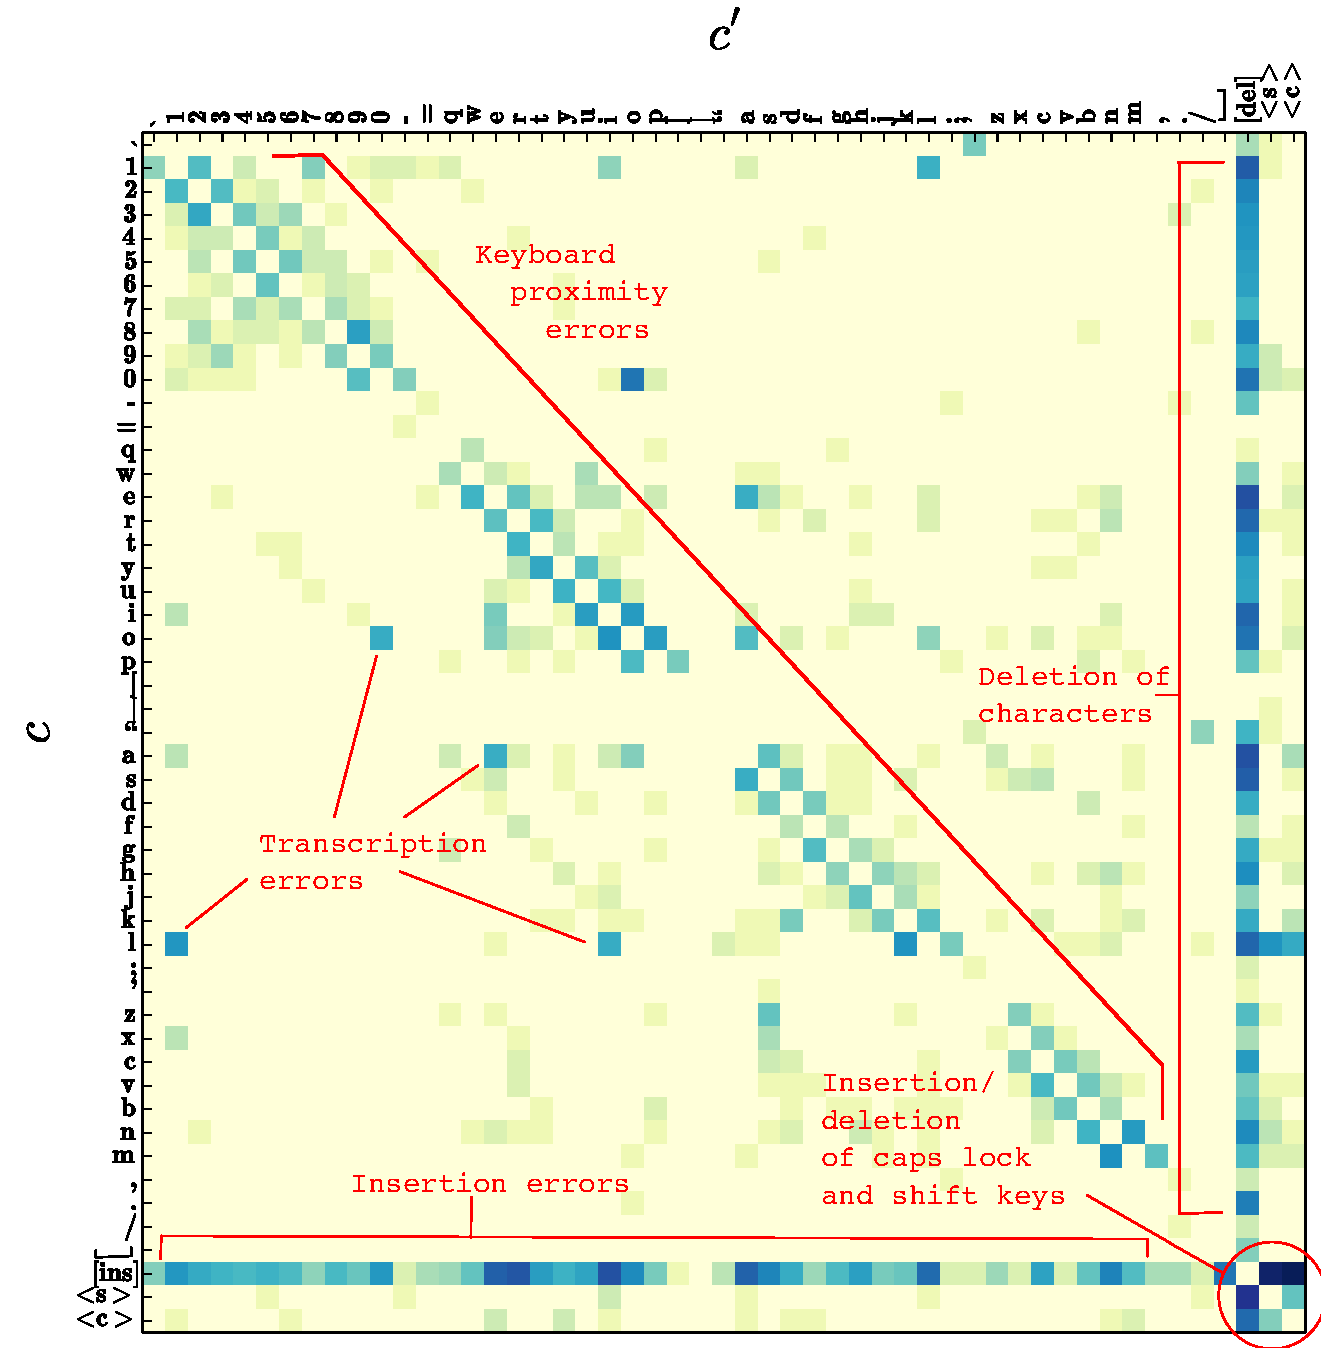
\includegraphics[height=0.48\textwidth]{images/heatmap}
  \caption{Heatmap showing the counts of edits that arose in computing
    \edistname from the key-press sequence of the submitted passwords
    to the key-press sequence of the prompted passwords. The color in
    row $c$ and column $c'$ indicates how often the edit
    $c \rightarrow c'$ was observed across all distance
    calculations. The darker the color the higher the count.  Labels
    [ins] and [del] denote insertion (character mistakenly inserted)
    and deletion (failure to type a character). Tokens \textvisiblespace $\,$, $\shift$, and $\caps$
respectively denote the and space-bar, shift, and caps lock.}
  \label{fig:heatmap}
\end{figure}


Several common typographical errors stand out:
\begin{newitemize} 
\item \emph{Insertion and deletion of shift and caps-lock keys}: In the right
  bottom corner appears a dark patch of $3\times3$ squares. This reflects the
  frequency of erroneous use or lack of use of shift and caps
  lock---equivalently, incorrect insertion or deletion of the $\shift$ and
  $\caps$ tokens.  These typos will switch the case of the password if it
  contains English letters as well as changing the shift status of digits and
  symbols (e.g., $4\rightarrow \$$).
  % (last two columns of the row $c=\mbox{[ins]}$) and deleted (last two
  % rows for the column $c=\mbox{[del]}$). 

%\item \emph{Number/symbol errors}: The diagonal in the symbol rows starting with
%$c = \textrm{@}$  reveal shifting errors in which symbols were accidentally typed as
%numbers. There is a symmetric diagonal showing numbers being mistakenly typed as
%symbols. 
%
\item\emph{Keyboard proximity errors}: The slightly darker cells near
  the diagonal represent typos due to mistakenly pressing a
  neighboring key to the left or right of the intended key.  
  We found more generally that there are a significant number of typos for which a key is
replaced by an adjacent one (left, right, above, or below).
  We collectively refer to these as proximity errors.

\item \emph{Number-to-number errors}: We see a
  square cluster of moderately high-frequency errors in the top left that represent digit-to-digit typos. Some of these are
  proximity errors, but many such errors confuse
  widely separated numbers, e.g., $3\rightarrow 9$.
  
%The bulk password characters are lower-case letters. \tnote{need more analysis --- nearby
%characters?}
\item \emph{Insertions and deletions}: There are throughout a large
  number of insertion (third row from the bottom) and deletion (third
  column from the right) errors. Deletions are slightly more common.
  %
\item\emph{Transcription errors}: The heatmap has sporadic dark cells, including
  \mbox{(l,1), (o,0), (0,o), (l,i)}. These represent transcription
  errors due to a worker confusing similar-looking characters. We presume that 
  the prevalence of reading errors are an artifact of the experiment design, and will be less frequent for entry of memorized passwords.
  Nevertheless, such errors could arise for users that write down 
  their passwords to remember them.
 % The worker got confused between to very similar looking
 % characters such as l (ell) and 1 (one).
\end{newitemize}
Our analysis suggests that a large fraction of common typos fall into a few
classes. A subset of these are what we refer to as ``easily correctable,'' as we
discuss shortly.

\subsection{Touchscreen Keyboards}
We performed a smaller, but similar, study in which workers were
required to use touchscreen keyboards. The hypothesis here is that the
distribution of typos may differ due to keyboard type. We submitted
24,000 passwords drawn from RockYou across 1,987 HITs using the same
methodology of approximately normalizing effort by restricting total
character counts to be less than 110.  Workers were given 300 seconds
to perform a HIT. We restricted workers to using touchscreen keyboards
by checking the {\tt user-agent} string of the worker's browser.

Unlike the desktop user experiment earlier in this section, we did not need to
adjust for the caps lock propagation error on touchscreen devices. This was
because of the fact that in touch screen devices the caps lock key is auto reset
every time the focus shifts from one input field to the other. We performed an
analysis that was otherwise similar to the analysis used above for the general
MTurk experiment. To calculate proximity errors, we used the Android keyboard
layout, which we believe is a sufficiently good proxy for all touch screen
keyboards.  

The probability of a typo here was 9.0\%, an increase over the 4.5\%
for unrestricted workers.  We compare the types of typos across the
two data sets quantitatively below.
 

\subsection{Easily-Correctable Typo Classes and Correctors}

Using all the data above we manually enumerate a set of common typo
types, or classes.  The resulting classes are detailed in
\figref{fig:top10-typo}, and shown for both the first general MTurk
experiment and the touchscreen-restricted experiment.  The column
labeled ``Corrector'' identifies the function that can be used to
correct the corresponding typos: $\swcall$ switches the case of all
letters in a password, $\swcfirst$ switches the case of the first
letter, $\rmlast$ removes the last character, $\rmfirst$ removes the
first character, and $\dtoslast$ changes the last character to its
equivalent character under the shift-key modifier (e.g., `1' becomes
`!', `a' becomes `A', etc.). The correctors mentioned above are
mutually exclusive, that is, any two correctors, when applied to an
input password of length larger than one, will produce two different
passwords (assuming at least one of the correctors is applicable).


\begin{figure}[t]
  \centering
  \small
  \begin{tabular}[t]{p{1.55in}lrr}
    \toprule
    \multirow{2}{*}{\textbf{Typo type}}     & \multirow{2}{*}{\textbf{Corrector}} & \multicolumn{2}{c}{\textbf{\% of typos}}\\\cline{3-4}
    &&\multicolumn{1}{c}{\textbf{Any\Tstrut}} &
    \multicolumn{1}{c}{\textbf{Mobile}} \\\midrule
    Case of all letters flipped & \swcall & 10.9 & 8.3\\
%    \midrule
    Case of first letter flipped & \swcfirst & 4.5 & 4.7\\
%    \midrule
    Added extra character to end & \rmlast & 4.6 & 0.9\\
%    \midrule
    Added extra character to front & \rmfirst & 1.3 & 0.5\\
%    \midrule
    Missed shift for symbol at end  &  \dtoslast & 0.2 & 0.1\\
    % \midrule
%    \midrule
    Proximity errors & n/a & 21.8  & 29.6\\
    %Character replaced w/ nearby character on US keyboard 
%    \midrule
    Transcription errors & n/a& 3.0 & 3.3\\
%    \midrule
    Other errors & n/a & 53.6 & 52.7\\ 
    % Upper case to Title case and vice verse  &  \upncap & 0.2 & 0.3\%\\
    % \rownumber. & \stodlast & Last character symbol-to-number & 1\%\\
    % Change the shift state of the last non-letter character & \swslast& 0.3\%\\
    \bottomrule
  \end{tabular}

%   \begin{tabular}[t]{p{2.0in}lrrr}
%     \toprule
%     \multirow{2}{*}{\textbf{Typo type}}     & \multirow{2}{*}{\textbf{Corrector}} & \multicolumn{3}{c}{\textbf{\% of typos}}\\\cline{3-5}
%     &&{\bf general} & \pbox{1in}{\bf general\\(adjusted)} & \pbox{.8in}{\bf touchscreen \\device} \\\midrule
%     Case of all letters flipped & \swcall & 30.9\% & 10.9\% & 8.3\%\\
% %    \midrule
%     Case of first character flipped & \swcfirst &3.8\% & 4.5\% & 4.8\%\\
% %    \midrule
%     Added extra character at the end & \rmlast &3.5\% & 4.6\% & 6.6\%\\
% %    \midrule
%     Added extra character at the front & \rmfirst &  1.3\% & 1.3\% & 1.1\%\\
% %    \midrule
%     Missed shift key for the last symbol &  \dtoslast & 0.2\% & 0.2\% & 0.0\%\\
%     % \midrule
% %    \midrule
%     Proximity errors & n/a & 17.3\% & 21.8\%  & 29.6\%\\
%     %Character replaced w/ nearby character on US keyboard 
% %    \midrule
%     Transcription errors & n/a & 2.3\% & 2.99\% & 3.4\%\\
% %    \midrule
%     Other errors & n/a & 41.0\% & 53.6\% & 45.7\%\\ 
%     % Upper case to Title case and vice verse  &  \upncap & 0.2 & 0.3\%\\
%     % \rownumber. & \stodlast & Last character symbol-to-number & 1\%\\
%     % Change the shift state of the last non-letter character & \swslast& 0.3\%\\
%     \bottomrule
%   \end{tabular}
  
  \caption{The top categories of typos observed in our MTurk experiments.  The
    ``Corrector'' column identifies an (easily applied) function that corrects
    the typo. The ``Any'' column is percentage of typos by category for the
    initial MTurk study in which workers could have used any browser. Of 97,632
    passwords drawn from RockYou, 4,364 were mistyped.  The ``Mobile'' column is
    the same for the 23,098 submitted passwords collected from devices with
    mobile browsers.  Of these, 2,075 had a typo. }
\label{fig:top10-typo}
\label{fig:top-typo-mobile}
\end{figure}



As can be seen, the distribution of typos is non-uniform. A few typo classes
account for a large proportion of mistakes made. Caps-lock errors alone
represent 9.2\% of all mistakes made in our general MTurk experiments, and
proximity errors for another 21.8\% of all mistakes.
For mobile, we see a proportionally larger number of keyboard
proximity typos.


If a class of typo has a uniquely determined associated corrector, we refer to
it as {\em easily correctable}. The typo that produces a flipped case in the
first letter is an example: The corresponding corrector just flips the case of
the first letter. Not all easily correctable typos have involutory correctors
(the typo and corrector are the same function): consider the case of adding a
character to the end of a password which is corrected by removing a character. 

In contrast to easily correctable typos, a proximity error is hard to correct.
Given a password with a proximity error, correction would require
identification of the erroneous character as well as identification of the
nearby character that was the original, true one. Thus the space of possible
correctors for a proximity error is generally large. As we shall see later,
both security and performance are adversely impacted by searching large spaces
of correctors.


Our exploration culminates in the following two key results: {\em (1) Some typos
are significantly more common than others} and {\em (2) Many common typos are
easily correctable}. In the next section, we report on experiments at Dropbox
that verify that common, easily correctable typos arise frequently in practice.




%%%%%%%%%%%%%%%%%%%%%%%%%%%%%%%%%%%%%%%%%%%%%%%%%%%%%%%%%%%%%%%%%%%%%%%%%%%%%%%%
% JUNKYARD
%%%%%%%%%%%%%%%%%%%%%%%%%%%%%%%%%%%%%%%%%%%%%%%%%%%%%%%%%%%%%%%%%%%%%%%%%%%%%%%%

% pop_long_complex 1 85
% pop_long_moderate 45 4221
% pop_long_simple 350 44515
% pop_med_complex 58 5781
% pop_med_moderate 5332 733006
% pop_med_simple 8262 2251869
% pop_small_complex 47 3920
% pop_small_moderate 6645 1025830
% pop_small_simple 21831 5965621
% unpop_long_complex 199860 207824
% unpop_long_moderate 733613 796593
% unpop_long_simple 631714 778742
% unpop_med_complex 560142 635361
% unpop_med_moderate 4155957 5921063
% unpop_med_simple 3301846 5025920
% unpop_small_complex 176363 220514
% unpop_small_moderate 2186662 3753303
% unpop_small_simple 2340753 5207152


\iffalse
\begin{figure*}[t]
  \gamesfontsize
  \label{table:RY-class-stats}
  \center
%  \begin{tabular}{c rrrr}
%    \toprule
%    \multicolumn{5}{c}{\RYpop}\\\toprule
%    & \RYsimple & \RYmoderate & \RYcomplex & Total\\\hline
%    \RYshort  &21,831 (5,965,621) & 6,645 (1,025,830) & 47 (3,920) & 28,523 (2,990,656) \\
%    \RYmedium &8,262 (2,251,869)  & 5,332 (733,006)   & 58 (5,781) & 13,652 (6,995,371)\\
%    \RYlong   &350 (44,515)       & 45 (4,221)&1 (85) & 396 (48,821)\\\hline
%    Total     &30,443 (8,262,005) & 12,022 (1,763,057)& 106 (9,786) & 42,571 (10,034,848) \\\bottomrule
%  \end{tabular}\\\bigskip

% % long_complex 199861 207909
% % med_simple 3310108 7277789
% % small_simple 2362584 11172773
% % long_moderate 733658 800814
% % med_moderate 4161289 6654069
% % long_simple 632064 823257
% % small_moderate 2193307 4779133
% % med_complex 560200 641142

  \begin{tabular}{c rrrr}
    \toprule
%    \multicolumn{5}{c}{\RYunpop}\\\toprule
    & \RYsimple & \RYmoderate & \RYcomplex & Total\\\hline
    \RYshort  & 2,362,584 (11,172,773) & 2,193,307 (4,779,133) & 176,363 (220,514) & 4,555,891 (15,951,906) \\
    \RYmedium & 3,310,108 (7,277,789)  & 4,161,289 (6,654,069)   & 560,200 (641,142) & 8,031,597 (14,573,000) \\
    \RYlong   & 630,064 (823,257)& 733,658 (800,814)&199,861 (207,909) & 1,565,583 (1,831,980)\\\hline
    Total     & 6,304,756 (19,273,819) & 7,088,254 (12,234,016)& 760061 (849,051)& 14,153,071 (32,356,886)\\\hline
  \end{tabular}\hspace*{0.2cm}

  % \begin{tabular}{|l|l|c|c|}
  %   \hline
  %   Feature & & unique passwords & users \\\hline
  %   \multirow{2}{*}{Popularity}& \RYpop &&\\
  %           &\RYunpop &&\\\hline
  %   \multirow{3}{*}{Length}& \RYshort &&\\
  %           & \RYmedium &&\\
  %           & \RYlong &&\\\hline
  %   \multirow{3}{*}{Composition} & \RYsimple &&\\
  %           & \RYmoderate && \\
  %           & \RYcomplex &&\\
  %   \hline
  % \end{tabular}
  \caption{Figure shows number of passwords in each of the classes we described
    above. In parentheses we have reported the number of users who used those passwords.  Most (94.3\%) of the passwords are of size less than 12
    characters, while less than one percent passwords comply with complex
    password policy.  }\rcnote{I dumped all the numbers. Obviously in paper we
    shall not put this. But this raises a question that how can we sample
    passwords for MTurk experiment.}
  \label{fig:group-summary}
\end{figure*}

\fi

%Exp 2: Remember what you are typing? (TODO: yet to be coded) Experiment 1
%simulates more of a transcribing environment than an ideal password typing
%environment where the user types password from their memory. In experiment two,
%we ask the workers to type each password 5 times in a row: first four of them
%they type while seeing the given password, but on the last time we hide the
%original password (See ~\figref{}).  We assumed if one types a password four
%times in a row, he/she should be able to memorize most of it and we monitor the
%typos while reproducing the password from memory. We also recorded the time
%taken to type each password. The worker are requested not to note down the
%given passwords. Every assignment comprises of total $k$ different passwords.
%We set an aggressive time limit for this experiment to discourage noting down
%the passwords.


%%% Local Variables:
%%% mode: latex
%%% TeX-master: "main"
%%% End:

%%%%%%%%%%%%%%%%%%%%%%%%%%%%%%%%%%%%%%%%%%%%%%%%%%%%%%%%%%%%%%%%%%%%%%%%%%%%%%%
\section{Experiments at Dropbox}
\label{sec:dropbox}

Our Mechanical Turk experiments in the last section show that there exists a
small set of frequently observed typos. Those experiments, which asked users to type
in passwords provided to them, may not simulate the kinds of typos users make
when using their own passwords. We therefore turn to investigating typos in the
production password authentication environment used at Dropbox. We will also
assess the impact of typos on user experience. We emphasize that our experiments
here did not change the effective login checks at Dropbox, but only recorded
information about the frequency of typos. 

\paragraph{The Dropbox authentication system.} Dropbox is a file
hosting service for consumers and enterprises with hundreds of
millions of users. Each user must select a password during
registration. Dropbox uses zxcvbn~\cite{dropbox2012zxcvbn}, a password
strength estimator, to guide the user in choosing a strong
password. The system requires that users choose a password of at least
six characters, but it does not explicitly forbid users from choosing
passwords that are considered to be weak by zxcvbn. Passwords are
submitted over a standard HTTPS POST interface when logging in via the
website or from within one of the native Dropbox applications. We call the
submission of a password by a user a {\em password submission}.  If the
password is accepted by the Dropbox server, we call it a  successful
password submission, otherwise it is called a failed password
submission.  On a failed password submission, the user may resubmit his/her
password. A {\em login attempt} is a sequence of password submissions by a user that either
culminates in a successful login, in which case the login attempt is considered successful, or accumulates login failures until the study ends. If
the user does not
succeed in logging in during the scope of our study, we consider her sequence of password submissions to be a failed login attempt.


Dropbox, like most modern web companies, uses a number of fraud detection
mechanisms in order to filter out spurious login attempts even before checking
the password. An example of such fraud detection mechanisms is to refuse login
attempts from IP addresses that appear on a blacklist for known bots. While
some spurious login submissions may make it through these filtering mechanisms,
we assume for simplicity below that our instrumentation is only monitoring
legitimate login attempts. Note that this is a conservative assumption: if the
data we collected contains illegitimate login attempts, then the true rate of
correctable typos for legitimate users would be even higher. Our security analyses
(\secref{sec:security}) will not make such assumptions.
%For the purposes of our study below, we assume any password login attempt We
%assume this does a good job at filtering 


\iffalse
lowercase first character, uppercase first character, remove first character, remove last character, swap case of entire password
\fi


%\tnote{Below I am using typo to refer to corrections. We need to make a pass to
%render homogenous the terminology and notation.}


\paragraph{Instrumentation.} We modified the Dropbox password checking code to
perform additional checks on all legitimate login attempts on the web
interface. This provided a vast amount of data, and it eliminated biases that
could arise from selecting some small percentage of accounts. This also made visible multiple password submissions from a single user, which was necessary for timing
re-tries.

During the period of measurement, every password submission was
processed as follows. If the password check passed, do nothing.
Otherwise, if it failed, apply one or more typo corrections from some
predefined corrector function set $\typoset = \{f_1,f_2,\ldots,f_c\}$
where corrector functions were defined in the last section. We used
slightly different sets of correctors in different experiments, as
discussed below.  One or more of the corrected version(s) of the
password are checked. For failed login attempts, a log entry was
generated that contained a time stamp, whether login would have been
successful with a correction of the password, the type of correction $f_i$
that was successful (if applicable), and the user agent string.

We emphasize that in our experiments login is \emph{not} allowed based on the
corrected passwords. We did not modify Dropbox's effective login checks; we
only collected the data needed to evaluate whether doing so would be
beneficial.


\paragraph{Typos and login failure rates.} In an initial experiment we
set out to measure the incidence rate of the top five corrections seen
in the MTurk study of \secref{sec:mturk}. Thus for this
experiment the set of corrector functions is
$\topfive = \{\swcall,\swcfirst,\rmlast,\rmfirst,\dtoslast\}$.  For
each instrumented failed password submission, one correction from
$\topfive$ was chosen uniformly at random and applied to the submitted
password.  The reason is that, in the current implementation, only
sequential code is easily supported, and the password hashing scheme
used at Dropbox is (by design) slow to compute. It was unclear a
priori exactly what overhead the additional checks would have on
Dropbox infrastructure, and so we conservatively only performed one
additional check at a time.
%ensured that latency of failed login
%attempts was only modestly increased, while still allowing us to collect
%aggregate statistics on the prevalence of each of the typos checked for overall.
The success of this initial experiment suggested the performance impact was low,
and later experiments applied multiple corrections (see below).
We collected information over a 24-hour period.

We cannot report on the exact number of login attempts during this
period, as this is considered confidential information by Dropbox. We will
therefore report only rates of success and failure.
% Dropbox
%has upwards of 
%\item %more than \fixme{500 million} customers, with one percent of users therefore
%being in the order of millions of customers. 
%The number of instrumented login attempts over the 24 hour period was
%\fixme{XXX}.  
%To make this clear, we need to fix some notation. 
In the following, we let $c_f$ denote the number of times a corrector $f$ was
applied to an incorrect password during an experiment. We let $r_f$  be the
number of times $f$ successfully corrected an incorrect password during the
experiment. The ratio $r_f / c_f$ gives the percentage 
of login failures correctable by $f$.


%Let $n$ be the total number of password submissions to the Dropbox
%authentication server in the 24-hour period, $a$ be the number of
%accepted password submissions, and $r$ be the number of rejected
%password submissions. For each incorrect password submission, one of
%the correctors is selected at random and used to correct the submitted
%password. Let $c_f$ be the number of times a corrector $f\in\topfive$
%is selected and $r_f$ be the number of time the correction was
%successful. Then, $ n = a + r = a + \sum_{f\in\topfive} c_f \;.$
%The ratio $r_f / c_f$ gives an estimate of the percentage of typos correctable
%by $f$. 
% Number of rejected submissions that could be corrected by
% $f \in \topfive$ is denoted by $r_f$, all other rejected submissions
% that cannot be corrected by any $f\in\topfive$ are denoted by
% $r_\textnormal{other}$.  Thus \bnm n = a + r = a + r_\textnormal{other} +
% \sum_{f\in\typoset} r_f \;.  \enm Now, let $r'_f$ be the measured
% number of password submissions that were correctable by $f \in \typoset$. Because
% we choose one corrector at random from $\topfive$ for each failed
% password submission, this measured number is not equal to the true
% number.  We can however estimate $r_f$ by $\hat{r}_f = |\topfive| \cdot r'_f = 5\cdot r'_f$.
% As mentioned, confidentiality concerns prevent us from reporting absolute
% numbers.

%, we report in the middle column
%the measured number of password submissions corrected by the corrector
%$f$ as a fraction of the total number of failed login attempts. In the
%far right column we give $r_f/c_f$, that is the estimated fraction of
%typos that can be corrected by the corrector $f$. The fraction of time
%a corrector is chosen is very close to 20\% for each corrector, hence
%we omit that column from the table.

% \footnote{Multiplication was performed before rounding, 
% so the latter column is not always exactly a multiple of five of the first
% column.}
% $\hat{r}_f / r = 5 \cdot r'_f/r$.

\pgfplotstableread[col sep=comma, format=inline] {
index,type,mobile,desktop
0,\swcall,0.383,1.21
1,\swcfirst,5.88,5.51
2,\rmlast,1.87,2.06
3,\rmfirst,0.390,0.347
4,\dtoslast,1.82,0.0367
}\devicedist

\begin{figure*}[t]
% \label{fig:dropbox-summary-one}
\begin{center}
\hpagesss{0.3}{0.3}{0.3}{
\vspace{0.3in}
\begin{tabular}{lr}
  \toprule
  Corrected by ($f$) & { $r_f/c_f$ (\%)}\Tstrut  \\
  \midrule
  $\swcall$   & 1.13\\ % & 1.13 \\
  $\swcfirst$ & 5.56\\ % & 5.56 \\
  $\rmlast$   & 2.05\\% & 2.05 \\
  $\rmfirst$  & 0.35\\ % & 0.35 \\
  $\dtoslast$ & 0.21\\ % & 0.21 \\
  \midrule
  $\topfive$   & 9.30\\ % & 9.30 \\
  \bottomrule
\end{tabular}}{
\vspace{0pt}
\begin{tikzpicture}[scale=0.5]
  \begin{axis}[
    axis y line=left,
    axis x line=bottom,
    ymin=0, ymax=6,
    xlabel={\Large Corrector $f$},
    ylabel={\Large \% of failures corrected ($r_f/c_f$)},
   %    y axis style=black!75!black,
    xtick=data,        
    xticklabels from table={\devicedist}{type},
    % xtick={{\large \swcall}, {\large \swcfirst}, {\large \rmlast}, {\large \rmfirst}, {\large \dtoslast}}
    legend style={at={(0.97,0.97)}, anchor=north east},
    ybar,
    enlarge x limits=0.3,
    % cycle list={
    % {fill=black!50,draw=black!50},
    % {fill=black!80,draw=black!80},
    % }
    ]
    \addplot [  black,
    fill=blue!40,
    postaction={
      pattern=north east lines
    }] table [x={index}, y={desktop}]  \devicedist;
    \addplot table [x={index}, y={mobile}]  \devicedist;
    \legend{Desktop, Mobile}
  \end{axis}
\end{tikzpicture}}{
% \label{fig:delay-cdf}
\vspace{0pt}
\begin{tikzpicture}[scale=0.5]
  \begin{axis}[
      axis x line=bottom,
      axis y line=left,
      xmode=log,
      xlabel={\large Time delay (s)},
      ylabel={\large \pbox{2in}{Fraction of users \\w/ multiple login attempts}}
      ]
      \addplot [blue, mark=none] table [col sep=comma,
      x=fraction of users, y=seconds saved] {images/cdf.csv};
    \end{axis}
  \end{tikzpicture}}
\end{center}
%\begin{tabular}{lrr}
%\toprule
%   Corrected by ($f$)& { $r_f/r$ (\%)}\Tstrut & { $r_f/c_f$ (\%)} \\
%\midrule
%$\swcall$   & 0.226  & 1.13\\ % & 1.13 \\
% $\swcfirst$ & 1.112  & 5.56\\ % & 5.56 \\
% $\rmlast$   & 0.407  & 2.05\\% & 2.05 \\
% $\rmfirst$  & 0.070  & 0.35\\ % & 0.35 \\
% $\dtoslast$ & 0.043  & 0.21\\ % & 0.21 \\
%\midrule
% $\topfive$  & 1.858  & 9.30\\ % & 9.30 \\
%\bottomrule
%\end{tabular}
%}
  \caption{\textbf{(Left)} The fraction of failed logins correctable
    by $\topfive$ in a 24-hour study at Dropbox. \textbf{(Middle)}
    Performance of $\topfive$ on mobile versus desktop. For each
    corrector in $\topfive$ we plot the fraction of failures for each
    platform correctable by the corrector. \textbf{(Right)} CDF of
    time delay (in seconds) between the first failed login due to a
    typo and first successful login. Included are only users that had
    a failed login attempt and later a successful one.
%$\topfive$.
  %in $\topfive$, chosen uniformly, would
  %have enabled login. 
  %Here $r$ is the number of failed login attempts,
  %$c_f$ is the number of times the corrector $f$ is selected to
  %correct the submitted password, and $r_f$ is the number times the
  %correction was successful. 
  %The observed and estimated fraction of
  %failed login attempts that can be corrected are
  %tabulated in the middle and the right column respectively.
  % The middle column is
  % the fraction of failed login attempts observed to be correctable the
  % corrector, and the far right column reports the estimated fraction
  % of failed logins that are correctable by the corrector. 
}
\label{fig:dropbox-summary-one}
\end{figure*}

%We give the breakdown of the measured rate of corrector function   
%A summary of the main statistics regarding failure rates and typo
%rates are given in \figref{fig:dropbox-summary-one}.


%$\cup \{\otherfail\}$ where $\otherfail$ is a catch-all for failed logins that 
%weren't detected as correctable (either they were not a typo correctable by a
%mechanism in $\typoset$ or was a typo correctable by one of the corrections in
%$\typoset$ that was not selected for that login attempt).  
%Thus $\hat{n} = 1 = \hat{s} + \hat{f}_\otherfail +
%\sum_{T\in\typoset} \hat{f}_T$.  Then because we sample randomly from
%$\typoset$, we expect that 

%rate of correctable failures of any type in $\typoset$ can
%be estimated by $|\typoset|\cdot\sum_{T\in\typoset}\hat{f}_T/\hat{n}$.  The rate
%of typo failures of a certain type $T\in\typoset$ is estimated by
%$\hat{f}_T/\hat{n}$. 


The left figure of \figref{fig:dropbox-summary-one} reports
the measured ratios $r_f/c_f$ for each corrector in $\topfive$ in
during the 24-hour period. 
This reveals that 9.3\% of failures are due to typos correctable by
$\topfive$, suggesting that typos indeed account for a significant
number of failed (legitimate) password submissions\footnote{We can add
  the fractions of typos because our correctors are mutually
  exclusive.}. By correction type, we see that the
most common correction (switching the case of the first character)
accounts for 60\% of these, and the first three (switching the case of
all characters, just the first character, dropping the last character)
account for over 90\% of these. Apparently capitalization errors are a
significant source of errors, which provides evidence for why Facebook
accepts these typos.

Some disparity with the MTurk results is apparent. While the top three of
these five correctors are the same, the ordering is distinct, with caps-lock errors
proportionally higher in MTurk then here. We believe this is due to the MTurk
experiment design, and that the Dropbox numbers more accurately reflect rates in operational environments.

While collecting this data, we recorded the user agent for all
password submissions, so we were able to analyze the performance of
typo correction on mobile platforms versus desktop platforms.  We
found that the estimated correction rate for mobile was slightly
higher at 10.5\%, compared to 9.3\% for desktop (calculated here with
the denominator being the number of rejected password submissions for
mobile and desktop, respectively). We show, in the middle figure of
\figref{fig:dropbox-summary-one}, the estimated correction rates for
each user agent broken down by corrector function.  We see that
\dtoslast is a significantly more effective correction on mobile,
which may be because mobile keyboards require switching to an
alternate keyboard to reveal symbols.  We also see that \swcall is a
more effective correction on desktop, most likely because it's easier
to leave caps lock enabled on conventional keyboards.\footnote{On
  Android devices, enabling caps lock requires pressing and holding
  the shift button, and on iPhone devices one has to double press the
  shift button to enable caps lock.}  %% Looking
%% ahead to the next section,
This dichotomy suggests the potential merit
of applying different correction policies on the server based on the
user agent. We leave the further analysis of this for future work. 


% \pgfplotstableread[col sep=comma, format=inline] {
% index,type,mobile,desktop
% 0,\swcall,0.383,1.21
% 1,\swcfirst,5.88,5.51
% 2,\rmlast,1.87,2.06
% 3,\rmfirst,0.390,0.347
% 4,\dtoslast,1.82,0.0367
% }\devicedist

% \begin{figure}[t]
%   \centering
%     \begin{tikzpicture}[scale=0.5]
%       \begin{axis}[
%         axis y line=left,
%         axis x line=bottom,
%         ymin=0, ymax=6,
%         xlabel={\Large Corrector $f$},
%         ylabel={\Large \% of failures corrected ($r_f/c_f$)},
% %        y axis style=black!75!black,
%         xtick=data,        
%         xticklabels from table={\devicedist}{type},
%         %xtick={{\large \swcall}, {\large \swcfirst}, {\large \rmlast}, {\large \rmfirst}, {\large \dtoslast}}
%         legend style={at={(0.97,0.97)}, anchor=north east},
%         ybar,
%         enlarge x limits=0.25,
%         %cycle list={
%         %  {fill=black!50,draw=black!50},
%         %  {fill=black!80,draw=black!80},
%         %}
%         ]
%         \addplot [  black,
%         fill=blue!40,
%         postaction={
%           pattern=north east lines
%         }] table [x={index}, y={desktop}]  \devicedist;
%         \addplot table [x={index}, y={mobile}]  \devicedist;
%         \legend{Desktop, Mobile}
%       \end{axis}
%     \end{tikzpicture}
%     \caption{Performance of $\topfive$ on mobile versus desktop. For
%       each corrector in $\topfive$ we plot the fraction of
%       failures for each platform correctable by the corrector.}
%   \label{fig:device-dist}
% \end{figure}



%Of the \fixme{12\%} of failed login attempts, we estimate that 
%to 
%We saw a significant number of failed login attempts at \fixme{20\%} of all
%login submissions. Still measuring relative to all login attempts,
%\fixme{$\hat{f}_T = 10\%$} were absolutely seen caught as one of the typos seen.
%This is \fixme{50\%} of all failures, suggesting that typos indeed account for a
%significant number of failed legitimate login attempts. 
%, \fixme{20\%} of submitted passwords failed to be correct and

%In \figref{fig:dropbox-summary-one} we provide a breakdown of the observed
%typo rates for those checked in $\topfive$. We see that caps lock is by far the
%largest fraction of typo errors, with first-character capitalization being the
%second most frequently occurring. The top three typos account for \fixme{80\%}
%of observed typos.  
%Note that because we probabilistically check one typo in $\topfive$, some
%numbers must be extrapolated.


\paragraph{Utility of the top three corrections.} We perform a second
study that restricts attention to just the overall top three
correctors $\topthree = \{\swcall,\swcfirst,\rmlast\}$ observed in the
previous study (and, in turn, the MTurk experiments). For this
experiment, the instrumentation applied all three correctors to any
password that failed to exactly match the registered password. So,
now $c_f$ is the number of failed login attempts for every $f \in \topthree$. %and
% so we no longer need to correct by a factor of $|\topthree|$ to perform
% estimates; the measured rate $\hat{r}_f / r$ is all what we need.
As before, we recorded data for 24 hours.

We additionally recorded the time duration for a login attempt to
succeed. That is the time lag between the first failed submission and
the first successful submission by each user in this 24-hour
period. (Because Dropbox uses session cookies most users typically
need to successfully login only once per 24-hour period.) This allowed
us to quantify the time delay between failures and successes, a
measure of how much utility is lost due to usability issues such as
typos.

As we would expect, the success rate of corrections closely matched
the results of the previous 24-hour experiment. Specifically, typos correctable
by $\topthree$ accounted for 9\% of failed password submissions. 
This also attests the stability of these percentages over time.

We show in right figure of \figref{fig:dropbox-summary-one} a CDF of
the delay in logging in over all users who eventually succeeded at
logging in (within the 24-hour period).  Note that some small fraction
of users did not log in for a very long time, suggesting they gave up
and came back hours later. Even so, almost 20\% of users that
experienced a failed login would have been logged in a minute earlier
should typo-tolerant checking have been enabled. Aggregated across all
failed login attempts, typo-tolerance here would have \emph{increased
  logged in time by several person-months just for this 24-hour
  experiment}.
%{\bf \textcolor{\notecolor}{$\ll$Anish: {\sf This ``several person-months'' is
%slightly misleading, because it takes into account those people who tried, say,
%logging in at 1pm (and got close enough with their password), but failed to log
%in, gave up, and came back a couple hours later... that isn't really a couple
%hours of wasted time. Should we get rid of this statement?}$\gg$}}
This represents a significant impact on
user experience and a clear pain point for companies keen on making it easy
for their users to log in.


In aggregate, of all users who attempted to log
into Dropbox within the 24-hour measurement period, we discovered that 3\% were turned
away even though at least one of their submitted passwords was
correctable by one of the correctors in $\topthree$. % Allowing typo
% tolerance with correctors in $\topthree$ would have increased the
% number of successful logged in users by a significant amount. 
This
also represents a significant impact on user experience, with users being
prevented from using the service.

% Every day, some users attempt to log in and use Dropbox, but they give up
% before successfully authenticating. Of the total number of people who visit the
% site in a 24-hour period with the intent of logging in, 3\% of the attempts are
% preventable failures: situations where the user gave up before successfully
% logging in, but where one of their password attempts was close enough
% (correctable by one of the three corrections) to have been logged in 
% were typo correction enabled. This also represents a significant
% impact on user experience, with users prevented from using the product.
% %when they could have been logged in with negligible impact on security.


\iffalse
\bigskip
\bigskip



\begin{newenum}
\item Description of basic experiment.  Explain
statistical sampling
\item Basic stats on rate of failed logins, percentage caught by typo checks
\item Experiment two: determining time saved and such
\end{newenum}

The experiments on MTurk discussed in the previous section provide a potential
model of the distribution of typos seen in practice. As previously noted, those
experiments however have some limitations, in particular the ecological validity
of the experimental MTurk procedure may not hold. Most obviously, that the types
of typos made differ for memorized versus transcribed passwords. 

In this section we report on at-scale experiments performed on Dropbox's
production password checking infrastructure. We perform hypothesis testing to
show that the distributions of typos that we come up using the data collected
from Mechanical Turk experiment is very close. \\

We want test following hypothesis -- 
\begin{itemize}
\item Are the percentage of total mistyped password in Mechanical Turk and that in
  Dropbox server same?
\item Are the most probable typos and their percentages similar across experiments?
\item Can the security analysis using RockYou password leak be generalized for
  other password distribution, especially the one of Dropbox? It will great if
  we can validate this, but probably we cannot.
\end{itemize}


[[What do we want to do to analyze the results of MTurk study?]]
[[Chi-squared to show that things match... use other for tail and we should have
a small categorical support]]
\fi


%%% Local Variables:
%%% mode: latex
%%% TeX-master: "main"
%%% End:

%%%%%%%%%%%%%%%%%%%%%%%%%%%%%%%%%%%%%%%%%%%%%%%%%%%%%%%%%%%%%%%%%%%%%%%%%%%%%%%%%
\section{Modeling Typos and Password Checkers}
\label{sec:formal}


In the past sections we saw that typos account for a large fraction of login
failures. This burdens users and can even cost companies money because users end
up not engaging with their services. We've also seen how correcting passwords on
user behalf can efficiently increase usability. The remaining question is
whether one can do so securely. We now answer this question. 

We start by giving a formal framework for typo-tolerant password checking, and
show how to realize the checking schemes suggested by our studies above. We
will also show, via what we refer to as the ``crossover theorem'' that one can
often build typo-tolerant checking schemes for which there is \emph{no security
loss}. This theorem depends upon the nature of the distribution of passwords 
and so we finally turn to empiricism using password leaks to investigate show
that typo-tolernace comes with insignificant security loss for the kinds of 
passwords used in practice.

%We will also introduce more subtle mechanisms, such as blacklisting of popular
%passwords 

%we give a framework for reasoning about and specifying typo-tolerant password checkers. 
%We will formalize the notion of
%a typo model, which captures the probability of particular errors
%arising across a user population. We will then describe a design for 
%typo-tolerance that takes advantage of a typo distribution model to efficiently
%check for high-probability typos. Along the way we will define the threat model
%and highlight the key issue with typo-tolerance:  the trade-off between
%usability and security.

\iffalse
A distance measure $\dist$ is a function
$\dist\Colon\PW\times\PW\rightarrow\R^+$.  We will often denote
$\dist(\pw,\pwtypo)$ by $\dist_\pw(\pwtypo)$.  The neighborhood of
$\delta$-close points of a password $\pw \in \PW$ is the set
$\ball_{\dist,\delta}(\pw) = \{\pwtypo \;|\; \pwtypo \in \PW
\textnormal{ and } \dist_\pw(\pwtypo) \le \delta\}$.
When $\dist$ and $\delta$ are clear from context we will write simply
$\ball(\pw)$ and call this the ball centered at $\pw$.
\fi

\subsection{Typos, balls, and neighborhoods}
\paragraph{Typo model.} Let $\PW$ be the set of all passwords, i.e., strings
over some alphabet $L$ up to a maximum length $\pwlength$. We might take
$L$ to be the set of all printable ASCII characters and the maximum length $\pwlength$ to be
sufficiently large to encompass user-selected passwords, e.g., $\pwlength = 64$. We associate with $\PW$ a
distribution~$\pwprob$ that models the probability of user selection of
passwords; thus $\pwprob(\pw)$ is the probability that a user selects a given password $\pw$. We assume for simplicity that passwords are independently drawn from~$\pwprob$. 

A key feature of our approach is that we do not appeal to a lexicographic notion of distance (e.g., Levenshtein distance) to model typos. Instead, we rely on a simple, key observation: Some typos are more likely than others. Thus we reason about typos in terms of probabilities, rather than distances. Specifically, we let $\typoprob_{\pw}(\pwtypo)$ denote the probability that upon authenticating, a user with password $\pw$ types $\pwtypo$. (If $\pwtypo \neq \pw$ then $\pwtypo$ is a typo; $\typoprob_{\pw}(\pw)$ is the probability that the user makes no typo.) We write $\pwprob(P)$ to denote the aggregate probability on a set $P \subseteq \PW$ of passwords.

For all $\pw \in \PW$, then, $\typoprob_\pw(\cdot)$  defines a probability space
over $\PW$. That is, $\typoprob_\pw(\pwtypo) \in [0,1]$ for any $\pwtypo$ and 
$\sum_{\pwtypo \in \PW} \typoprob_{\pw}(\pwtypo) = 1$. In practice, generally $\typoprob_\pw(\pw) > 0$, i.e., users will sometimes enter passwords correctly. Also, for many password pairs, $\typoprob_{\pw}(\pwtypo) \neq \typoprob_{\pwtypo}(\pw)$. For example, a user may mistype her password $\pw =$ ``Unlockme'' as $\pwtypo =$``unlockme'' as a result of accidentally failing to depress the SHIFT key, while a user whose password is $\pwtypo =$``unlockme'' is less likely to press SHIFT accidentally and capitalize the letter `u'.

Implicit in our model is the simplifying assumption that typos depend only on a user's password $\pw$ and
not, for example, on the user that typed them, the time of day, or other factors.
As we will see, this assumption simplifies operationalization of typo
tolerance models. As one example, modeling individual users' typo habits would require a server to record the user's typo history.
While higher-accuracy correction for the user might then be possible, this feature would, of course, result in a more complex system. It could also leak password information: Recoding the fact that a user fails to capitalize the first character in her password leaks the fact that that character is a letter.

\paragraph{Neighborhoods.} We define the neighborhood $\nh{\pw}$ of a password
$\pw$ as the set of passwords that a user with $\pw$ may type in attempting to
enter $\pw$. Thus $\nh{\pw} = \{\pwtypo \,|\, \typoprob_{\pw}(\pwtypo) > 0\}$. 

Some passwords in $\nh{\pw}$ may have very low associated probabilities,
reflecting typos that rarely occur in practice. In this paper, we focus on and
characterize common typos, so a more restrictive definition of neighborhoods is
helpful. We define a {\em mutation} $\mut: \PW \rightarrow \PW$ as a (possibly
randomized) function that models a specific form of typo. For example, $\mut$
might flip the case of the first letter in $\pw$, modeling the form of typo in
the example above that transforms $\pw =$ ``Unlockme'' into $\pwtypo
=$``unlockme.'' 

Let $\mutset = \{\mut_0, \mut_1, \ldots, \mut_{a-1}\}$ denote a set of $a$
mutations, where $\mut_0$ is specially designated as the identity function
(modeling correct entry of a password). We let $\newnh{\pw} =
\{\mut_i(\pw)\}_{i=0}^{a-1}$ denote the {\em mutation-set neighborhood} induced
by the set $\mutset$ of mutations. This restricted definition of a neighborhood
is helpful in reasoning about common typos. We use the term ``neighborhood''
rather than ``mutation-set neighborhood'' where the context is clear.

\paragraph{Balls.} We define the {\em ball} of a password / typo $\pwtypo$ as
the set of passwords $\ball(\pwtypo) = \{\pw \,|\, \pw \in \PW \mbox{ and }
\typoprob_{\pw}(\pwtypo) > 0\}$.  Given a submitted password $\pwtypo$,
therefore, $\ball(\pwtypo)$ is the set of passwords $\pw$ that a user {\em might
have meant to type when actually entering $\pwtypo$}. 

A ball may be thought of as the inverse of a neighborhood: If $\pwtypo \in
\nh{\pw}$, then $\pw \in \ball(\pwtypo)$, and vice versa. Note that a ball may
lie outside the support of $\pwprob$: A password may never be registered by
users but still shows up as a typo.

Similarly, we may think of the inverse of a mutation as what we call a {\em
typo-corrector}, a (possibly randomized) algorithm $\tcf$ that takes as input a
password in $\PW$ and outputs a corrected password (also in $\PW$).  
For instance, $\tcf$ might correct the example mutation above in
which a user fails to capitalize a leading letter. In this case, if $\pw$ begins
with a letter $\ell \in L$, $\tcf(\pw)$  capitalizes $\ell$ and outputs the
result, while if $\ell$ is not a letter, $\tcf(\pw) \rightarrow \pw$. 

Just as some mutations may be especially common, making it helpful to reason in
terms of mutation sets, so typo-correctors may be especially helpful. In fact,
we focus on typo-correction strategies that employ just a few select
typo-correctors. We define a set of typo-correctors as $\tcfe = \{\tcf_0,
\ldots, \tcf_{\chbudget-1}\}$, where $\tcf_0$ is specially designated as the
identity function. We define the {\em typo-corrector ball}
$\newball_{\tcfe}(\pwtypo) = \{\tcf_i(\pwtypo)\}_{i=0}^{\chbudget-1}$.  We use
the term ``ball'' rather than ``typo-corrector ball'' where the context is
clear, and also write $\newball(\pw)$, dropping the subscript $\tcfe$ where
appropriate.

\paragraph{\em Remark:} While
$\pwtypo \in \nh{\pw} \Leftrightarrow \pw \in \ball(\pwtypo)$, of
course it is {\em not} the case that
$\pwtypo \in \newnh{\pw} \Leftrightarrow \pw \in
\newball_{\tcfe}(\pwtypo)$
for every $\mutset$ and $\tcfe$. Moreover, in practice some typos /
mutations that occur relatively frequently in practice are hard to
correct. This is true, for example, of the mutation $\mut$ that omits
the last letter of a password $\pw$ (which was among the top four most
common typos observed in our MTurk experiments, as reported
below). There is no effective general way to correct this typo, e.g.,
no deterministic typo-corrector $\tcf$ that corrects this typo for all
passwords.

\begin{figure*}[t]
\centering
\begin{minipage}[b]{.35\textwidth}
  \includegraphics[width=1\textwidth]{images/neighborhoods.pdf}\vspace{-7mm}
\caption{Neighborhoods for passwords ``Password!'' and ``Password1'' under example mutation set $\mutset$.}\label{fig:neighborhoods}
\end{minipage}\qquad
\begin{minipage}[b]{.35\textwidth}
 \includegraphics[width=1\textwidth]{images/ball.pdf}\vspace{-7mm}
\caption{Ball for password ``password1'' under example typo-corrector set $\tcfe$.}\label{fig:ball}
\end{minipage}
\end{figure*}

\paragraph{Example.} We give a simple example for a mutation set $\mutset = \{\mut_0, \mut_1, \mut_2\}$ such that $f_1$ flips the capitalization of the first letter of a password and $f_2$ changes a terminal symbol to a number,  and a typo-corrector set $\tcfe = \{\tcf_0, \tcf_1, \tcf_2\}$ where $\tcf_1$ and $\tcf_2$ that respectively fix $\mut_1$ and $\mut_2$. Figure~\ref{fig:neighborhoods} show neighborhoods for passwords ``Password!'' and ``Password1,'' while Figure~\ref{fig:ball} depicts the ball for ``password1.'' Note that the two neighborhoods include ``password1'' in their intersection, which is why ``Password!'' and ``Password1'' are both in the ball for ``password1.''

\subsection{Password checkers}
A password checker consists of two algorithms:

\begin{itemize}
\item $\register$ is a (possibly randomized) password registration function. It takes as input a password $\pw$ and outputs a string $s$ that may, for example, be the output of a password hashing scheme like scrypt. 
\item $\checker$ is a (possibly randomized) password verification function. It takes as input a password $\pwtypo$ and a stored string $s$, and outputs a boolean value, either $\accept$ or $\reject$.
\end{itemize}

More generally one might return a value
in $[0,1]$ which acts as a confidence in how close is $\pwtypo$ to the
registered password. This would be useful in systems that combine multiple
contextual authentication signals to make an authentication decision. We will
focus on the boolean case, but our techniques extend in natural ways
to confidence values (e.g., by returning $\typoprob_\pw(\pwtypo)$).  A
password checker is deterministic if $\checker$ is deterministic.

We measure utility of a typo-tolerant checker by the probability that
the checker outputs true for entered passwords, including some
typos. Formally, the acceptance utility is equal to
$\utility = \Pr[\ACC(\checker)\Rightarrow \true]$, where $\ACC$ is the random
variable defined by the output of the pseudocode experiment described
in \figref{fig:acc-security}. There $\getpwp$ means sampling from the
set according to $\pwprob$, and $\gettypo$ means sampling from the set
according to $\typoprob_\pw$.  The game is (implicitly) parameterized
by the scheme algorithms, the password distribution $\pwprob$, and the
typo model $\dist$.

\begin{figure}[t]
\center
\fpage{.20}{
   \underline{$\ACC(\checker)$}\\
   $\pw \getpwp \PW \next \pwtypo \gettypo \PW$\\
   $s \getsr \register(\pw)$ \\
   $b \getsr \checker(\pwtypo,s)$\\
  Return  $b$
}\hspace{0.1in}
\fpage{.20}{
\underline{$\ATT(\checker,\advA, q)$}\\[1pt]
$\pw \getpwp \PW \next s \getsr \register(\pw)$\\
$\advA^{\CheckOr}$\\
Return $\win$\medskip

\underline{$\CheckOr(\pwtypo,s)$}\\[1pt]
$b \getsr \checker(\pwtypo,s)$\\
If $(b = \true)$ then \\
\myind $\win \gets \true$\\
Ret $b$
}
\caption{(\textbf{Left}) Experiment for defining acceptance utility
  for a typo-tolerant checking scheme $\register,\checker$.
  (\textbf{Right}) Security game for online guessing attacks.}
\label{fig:acc-security}
\end{figure}

An \emph{exact checker} is one for which $\checker(\pwtypo,s)$ never outputs one
when $\pwtypo \ne \pw$ yet $s\getsr \register(\pw)$.  In practice of course,
exact checkers actually have a non-zero, but cryptographically small probability
of false acceptance (for typical hash-function-based checkers, this small
probability is equal to the probability of having found a collision in the hash
function).  We will throughout ignore this false acceptance probability.  We
note that the acceptance utility of an exact checker will always be less than 1
assuming that there exist $\pw$ and $\pw'$ for which $\pwprob(\pw) > 0$ and
$\typoprob_\pw(\pw') > 0$. That is, the probability of typos is higher than zero.

\paragraph{Typo-tolerant checkers.} We will primarily focus our 
attention on building typo-tolerant checkers that {\em relax} the checks made by an
existing exact construction. Let $\exregister, \exchecker$ be the algorithms of
an exact checker. Then an associated relaxed checker $\checker$ has the same
registration algorithm $\register = \exregister$, but is not exact, i.e., $\checker \neq \exchecker$.
Specifically, our approach will be to design a function $\register$ that individually checks each of {\em multiple candidate
passwords} in a set $S$ using $\exchecker$, where elements of $S \subseteq \ball(\pwtypo)$ represent possible typo corrections to a submitted password $\pwtypo$.

Relaxing an exact checker is a desirable approach to typo-tolerance
for two main reasons. First, it means that modifying a system to
become typo-tolerant can be done just by deploying a new checking
algorithm that works with previously registered passwords.  For
example registration may use a password hashing scheme like
scrypt~\cite{percival2015scrypt} or argon2~\cite{biryukov2015argon}, or use
a password onion construction that combines password hashing with an
off-system crypto service~\cite{everspaugh2015pythia}.

Second, from a security perspective, it implies that  compromise of the password
storage has the same effect as for the legacy system.  In particular brute-force
cracking attacks given~$s$ will work precisely as well as before. Of course,
should the typo-tolerant $\checker$ algorithm be very complex to implement, it might increase the likelihood of software implementation
vulnerabilities.  For this reason, we consider simple-to-implement relaxed checkers.
We emphasize that security could still be diminished by the adoption of relaxed checking, due to remote
brute-force attacks, a subject we will investigate in detail below.

Of course, relaxing an exact checker does come with limitations. We must run $\exchecker$ against each of the elements of the candidate set  $S \subseteq \ball(\pwtypo)$ until a match is found or none is found and $\pwtypo$ is rejected.\footnote{We note that this can be
  viewed simply as the standard brute-force construction of an error
  correction code from an error detection code.} As $\exchecker$ is designed to be
computationally expensive to thwart offline brute-force guessing attacks, this process may be slow if $|S|$ is large. We will show that one can significantly increase acceptance utility using a small set $S$ and thus few invocations of
of $\exchecker$ beyond the single one necessary to achieve perfect
correctness.

In \apref{sec:secure-sketches} we discuss some natural approaches to
typo-tolerant systems that use cryptographic constructions such as
secure sketches, but note that unfortunately these do not appear to
provide sufficient security in the face of server compromise.

\paragraph{A utility-optimized relaxed checker.} Let $pw$ denote the true password selected by a user. Then for a  submitted password (potential typo) $\pwtypo$, it is the case that $\Prob{pw = \pw \,|\, \pwtypo} = (\typoprob_{\pw}(\pwtypo) \pwprob(\pw)) / (\sum_{\pw'} \pwprob_{\pw'}(\pwtypo))$. Thus, for a given $\pwtypo$, see that $\Prob{pw = \pw \,|\, \pwtypo} \varpropto \typoprob_{\pw}(\pwtypo)\pwprob(\pw)$.

Suppose, then, that the checker designer has perfect knowledge of the distributions $\pwprob$ and $\typoprob$. 
Given a potential typographical error, i.e., $\pwtypo \gettypo \PW$, the following procedure to recover $\pw$ is possible. Order the set $\ball(\pwtypo)$ by nonincreasing value of $\typoprob_{\pw}(\pwtypo)\pwprob(\pw)$ and successively test each element of $\ball(\pwtypo)$ using $\exchecker$. If
$\exchecker$ finds a match, output $\true$ and stop, else continue
until $\ball(\pwtypo)$ is exhausted and output $\false$. Informally, this procedure is utility-optimal for a relaxed checker in the sense that, given $\pwtypo \gettypo \PW$: (1) It achieves $\utility = 1$ and (2) Among all possible relaxed checking procedures with $\utility = 1$, it achieves the minimum expected number of invocations of $\exchecker$.

Unfortunately, this procedure is impractical for a number of reasons. First, it requires a potentially huge number $|\ball(\pwtypo)|$ of 
invocations of $\exchecker$. Second, a checker designer in practice may not know $\pwprob$ and $\typoprob$ exactly, and may find it hard to estimate them for low-probability passwords or for all elements of $\ball(\pwtypo)$ (which may be large). Finally, as we have noted, there is a tension between utility and security in typo-tolerant password checking; it is not appropriate to optimize utility alone.

\paragraph{Our strategy: Relaxed checking with typo-correctors.} Given the (intentionally imposed) high computational burden of invoking $\exchecker$, achieving a practical checker design requires that only a relatively small set of candidate passwords be checked using $\exchecker$. We focus in this paper on the simple strategy of using a fixed set $\tcfe$ of typo-correctors in relaxed checking. When a password $\pwtypo$ is submitted, $\checker$ uses $\exchecker$ to test the sequence of passwords $\tcf_0(\pwtypo), \tcf_1(\pwtypo), \ldots, \tcf_{\chbudget-1}(\pwtypo)$ in order. If a match is found, $\checker$ outputs $\true$ and halts. If all checks fail, it outputs $\false$. This approach generalizes industry practice (\`{a} la Facebook, Vanguard, etc., as noted above) and, as we shall show, achieves a good balance between utility and security. 

\subsection{Security of relaxed checkers}
\label{subsec:security}
As discussed above, since we focus on relaxed checkers, attacks due to
compromise of an authentication server, such as offline cracking
attacks, are not affected by the change to typo-tolerance. The
critical question, then, is the effect of typo-tolerance on online
guessing attacks. 

Let us precisely define the notion of an online attack. In \figref{fig:acc-security} we give a simple guessing game
played between an adversary $\advA$ and a checker. The game $\ATT$ is
implicitly parameterized by $\pwprob$ and the checker
$\register,\checker$. The advantage of the adversary $\advA$ in
guessing the password is measured as
$\epsilon_\advA = \Pr[\ATT(\advA)\Rightarrow\true]$.  This security
game models a vertical attack, where the attacker tries to compromise
a randomly chosen user account; changing this security game to model
horizontal attacks is straightforward.  

First let us derive a bound on the optimal guessing attack given a
certain query budget~$q$.  Recall that if the checker is exact, we
have that $\epsilon_\advA \le \lambda_q$ for any $\advA$ making at
most $q$ queries where $\lambda_q = \sum_{i=1}^q \pwprob(\pw_i)$ 
for $\pw_1, \pw_2, \ldots$ in order of decreasing probability, i.e.,
that $\pwprob(\pw_i) \ge \pwprob(\pw_j)$ for $i < j$.  

Given a relaxed checker, in submitting a password guess $\pwtypo$, an
attacker induces checking on {\em all of the passwords in
  $\newball(\pwtypo)$}. We assume that given a $\pwtypo$, the attacker
can compute $\newball(\pwtypo)$. Intuitively, then, the optimal
strategy for an attacker for the game $\ATT(\advA,q)$ is to
iteratively guess the password $\pwtypo$ whose ball
$\newball(\pwtypo)$ has the largest aggregate probability over
passwords in $\PW$ not yet checked during the game.

More precisely, the strategy is as follows. Initialize a set
$P \gets \PW$ of possible passwords. Then repeat the following until
the query budget $q$ is exhausted. Guess a password $\pwtypo$ that
maximizes $\pwprob(\newball(\pwtypo) \,\cap\, P)$. If the query
succeeds, then the game is won; otherwise set
$P \gets P \setminus \newball(\pwtypo)$ and repeat.

Let the probability of success of this attacker be denoted by
$\fuzzlambda_q$. For $q=1$, we simply have
$\fuzzlambda_1 = \argmax_{\pwtypo \in \PW}
\pwprob(\newball(\pwtypo))$.
In other words, for $q=1$, an optimal attacker simply guesses the
password $\pwtypo$ whose ball has the highest aggregate probability,
i.e., for which $\pwprob(\newball(\pwtypo))$ is maximized. This
guessing strategy is analogous, in an exact-checking setting, simply
to guessing the most probable password. We observe that
$\fuzzlambda_1$ as defined here coincides conceptually with the fuzzy
min-entropy notion of Fuller et al.~\cite{fuller2014fuzzy}.

It is easy to see that this is optimal, meaning
$\epsilon_\advA \le \fuzzlambda_q$ for any $\advA$ making at most $q$
queries.  We can prove this in the following way. The optimal set of
$q$ guesses also contains optimal set of $q-1$ guesses for any
$q\ge 1$, so in other words. We have shown that $\fuzzlambda_1$ is
optimal. The, only thing remains to show is that if
$\fuzzlambda_{i-1}$ is optimal then, $\fuzzlambda_i$ is also optimal
for any $i\le q$. The attacker, at $i$-th iteration picks the password
that increases its success probability maximally, and as we assumed,
the previous $i-1$ guesses were optimal, i.e., $\fuzzlambda_{i-1}$ is
maximum advantage that an attacker can obtain with $i-1$ queries,
$\fuzzlambda_{i}$ will also be maximum. 

For this algorithm the time complexity is of the order of the size of
set $\PW$. We propose an alternative approach to restrict the search
space and improve the time complexity. Please see~\apref{sec:faster-attack}.

\paragraph{Worst-case security loss.} 
Let us start with the intuition for why typo-tolerance represents a potential 
security risk.  Assume for simplicity that $\pwprob$ is uniform over $\PW$ and that $\checker$ is such that
$|\newball(\pwtypo)| = \chbudget$ for all $\pwtypo$. Then moving to the typo-tolerant checker can increase the
probability of success of an online brute-force attacker (whether horizontal or
vertical) by a factor of $\chbudget$. Formally, 
$\fuzzlambda_q = \chbudget \lambda_q$ for all $q$ such that there exist $q$ disjoint balls.

It is tempting to conclude that typo tolerance will \emph{always} result in a
factor $\chbudget$ decrease in security. But this conclusion is too hasty:
$\pwprob$ is not uniform in reality and, in particular, passwords with high
mass are sparse in the universe $\PW$. Sparsity matters since a high
$\fuzzlambda_q$ depends intimately on finding passwords that are typos of many
high-probability passwords. 
%Let us look at another artificial example where there is in
%fact \emph{no} security loss. 

%\paragraph{The crossover theorem.} 
\paragraph{Free corrections theorem.} 
%While the artificial example above gives a worst-case bound on security loss, it
%is quite conservative and bears little on security in practice: human-chosen 
%passwords are not uniformly random. 
We would ideally like to have typo-tolerant checkers that
enjoy \emph{free corrections}. This means that  
its security is equivalent to the security of an exact checker.  
It is easy to come up with artificial distributions 
which admit free corrections of all typos. Specifically a distribution for
which no password's neighbor is in the ball of another password. 

Unfortunately, real password distributions do not enjoy this property. For
example, in the RockYou password leak and taking $\topfive$ as the set of
corrections to apply, one has significant overlap even amongst the  top 50
passwords. We therefore ask: for the password distributions seen in practice, 
can one achieve checkers with free corrections? The answer is yes as formalized
by the following theorem.

%hasIn particular, when no password's 
%We show that for most natural distributions one can get corrections ``for free'', at least when it
%comes to doing so without security loss. In words, the theorem below states that
%one can always build a typo-tolerant password checker such that acceptance
%utility increases over exact checking, yet the optimal advantage of an online
%guessing adversary is only as good as it would be against exact checking. 


\begin{theorem}[\textbf{Free corrections}] Fix $q > 0$, some password distribution
$\pwprob$ with support $\PWset$, 
a typo distribution $\dist$, and an exact checker $\exchecker$.
If there exists $\pw \in \PWset$ with a neighbor $\pwtypo$ for which
$\pwprob(\ball(\pwtypo)) < \pwprob(\pw_q)$,  then there exists a typo-tolerant
checker~$\checker$
for which $\ACC(\checker) > \ACC(\exchecker)$ and $\lambda_q = \fuzzlambda_q$. 
\end{theorem}


\noindent\emph{Proof:}
Consider the following typo-tolerant checker. Upon input $\pwtypo$, it first
checks whether the mass of the ball $p(\ball(\pwtypo)) > p_q$ where recall that $p_q$ is the
probability mass of the $q\thh$ most probable password (under
distribution~$\pwprob$). If it is larger, then only check $\pwtypo$ and do not
attempt typo correction. If instead the mass of the ball is smaller than $p_q$,
then check all passwords in the ball and accept the password if any match. Let
$\checker$ be the checker just described. 

Now we must prove two things about $\checker$. First that acceptance utility is
higher than just exact checking.  By assumption we have that the there exists
some password $\pw \in \PWset$ that has a neighbor $\pwtypo$ for which $0 <
p(\ball(\pwtypo)) < p_q$. Because this ball's mass is less than $p(\pw_q)$,
 $\checker$ will accept $\pwtypo$ while the exact checker will not. 
Thus $\ACC(\checker) \ge \ACC(\exchecker) + \pwprob(\pw)\cdot \dist_\pw(\pwtypo)$. 

%be that it includes a password $\pw \in \ball(\pwtypo)$ with $\pw \ne \pwtypo$
%and $\pwprob(\pw) > 0$.  This password will also have $\pwtypo$ corrected under
%$\checker$, since $\ball(\pwtypo) < p_q$. Noting that the exact checker will
%never correct this typo, we have that 



Now we prove the other part, that $\lambda_q = \fuzzlambda_q$. Assume for
contradiction that instead ... \fixme{Rahul you want to fill this in?}
\qedsym\\

A few comments are in order.  As $q$ increases, the mass of the neighbor's ball
must decrease for the proof to work. For relevant ranges of $q$ (e.g., $q \le
1000$), this condition will however be met for the highly-skewed password
distribution seen in practice. \tnote{do we want some empiricism here?} An
example setting that does not meet the conditions of the theorem is the
artificial one given above that has uniformly distributed passwords. %We note
%that this assumption is not strictly necessary for free corrections: one can
%give (again artificial) distributions which can have free corrections but do not
%meet the conditions. 

The typo-tolerant checker given in the proof may be inefficient (should balls be
very large), but it is easy to see that the checker can be made efficient by
only handling an efficiently checkable portion of any ball.  As long as that
portion contributes to improving acceptance utility, one still gets free
corrections.

A final issue is that the construction within the proof would be, as presented,
subject to timing attacks that leaks partial information about what password a user
entered to network attackers. This can be fixed easily by implementing the typo
checker in a constant-time fashion.

\iffalse
In the special case that no two password neighborhoods overlap and thus $|\ball(\pwtypo)| = 1$ for all $\pwtypo \in \PW$, it is possible to design a scheme $\checker$ with no security loss relative to the exact checker $\exchecker$ and with $\utility = 1$.

For any scheme $\checker$ (with $\utility \leq 1$), when no ball contains two passwords in the support of $\pwprob$, there is no security loss. It is easy to see that this is the case: Any password $\pwtypo$ submitted by an attacker results in at most one invocation of $\exchecker$ on a password that a user might select. In fact, there is no security degradation provided that $\fuzzlambda_q = \chbudget \lambda_q$. This much weaker condition is satisfied, for example, if the $q$ balls with the highest aggregate probabilities have the same probabilities as the $q$ most probable passwords. 

Intuitively, balls will not contain two distinct passwords $\pw, \pw'$ provided that these passwords do not have overlapping neighborhoods, a condition that occurs when the passwords are sufficiently ``distant'' from one another. Specifically, there should be no typo that maps $\pw$ onto password $\pwtypo$ and other typo that also maps $\pw'$ onto $\pwtypo$ such that $\checker$ corrects both typos. High lexicographic distance often achieves this condition in practice.

\iffalse
no two neighborhoods overlap,
typo tolerance comes at no security loss. In detail, consider a
distribution $\pwprob$ and typo model $\dist$ such that for any
$\pw,\pw'\in \PW$ with $\pwprob(\pw) > 0$ and $\pwprob(\pw') > 0$
there does not exist a $\pwtypo$ such that both
$\similar_\pw(\pwtypo) >0 $ and $\similar_{\pw'}(\pwtypo)> 0 $.  In
words, this just means that there exist no points in common between the
neighborhood of any $\pw$ and $\pw'$.  Then one can in theory build a
checker that achieves acceptance utility 1 and for which
$\fuzzlambda_q = \lambda_q$ for all~$q$.
\fi

This observation was made (using less formal reasoning) in prior
treatments on computer-generated
passwords~\cite{shay2012correct,techreport}, where one can have the
system arrange for all chosen passwords to be sufficiently ``distant''
from one another with respect to a reasonable typo model. But for
user-generated passwords it is unlikely that one gets such a
situation.

So we have two extremal, but artificial, examples of
security. Security loss could be as bad as a factor of $\chbudget$. It
could also come at no loss. The truth will be somewhere in between,
and here we must turn to empiricism. To start, we do a brief
exploration of the structure of real user passwords under a typical
distance measure, Damerau-Levenshtein distance.

\fixme{We will consider heuristics that enforce the condition that a correction ball contains only one  high-probability password. A simple one is this: If a known high-probability password is encountered while iterating through typo-correction functions, halt.}

\paragraph{Damerau-Levenshtein distance} Damerau-Levenshtein distance
is a widely used distance metric for spelling errors. This metric
evolved from the work by Levenshtein~\cite{levenshtein1966binary} and
Damerau~\cite{damerau1964technique}.  DL distance between two strings
is the minimum number of edit operations required to convert one
string into the other. Here allowed edit operations are insertion,
deletion, substitution and transposition.  Using simple dynamic
programming we can efficiently calculate DL distance between two
strings.  For our analysis we have used case independent DL distance,
where we compute the DL distance after converting both the string to
lower case.


\subsection{Sparsity of 1-DL Typos in Rockyou}
\fi




\tnote{There is a bunch of stuff commented out in latex below and in model.tex}

\iffalse

\bigskip
\bigskip
\bigskip

There are three main component of a typo tolerant password checking system. 
First, a fuzzy equality metric, that tells what is the probability that two
strings could be typo of each other.


\paragraph{Typo-tolerant password checking.}  
Typo tolerant password checking is the accepting passwords that are withing some
distance from the original password. Here, the distance is a function that maps
a pair of strings onto a real number.

\rcnote{
\begin{itemize}
\item Define {\em fuzzy-guess rank}, and {\em fuzzy-$\beta$ success rate}.
\item Formal definition of typo tolerance? \\
  The function {\tt fuzzy\_equal($w, \hat{w}$)} is an abstract function
  implemented by the servers that decides whether $\hat{w}$ can be treated as a
  proxy for $w$ for authentication or not.  In general this is just an equality
  checking, we can extended it to more flexible checks, e.g., treats the strings
  as equal if the DL-distance between the strings are under some limit.
\end{itemize}
}




\rcnote{random thoughts follow..}  However for typographical error correction we
have seen (shown in later section of the paper) several issues with simple edit
distance. Firstly, ``password'' and ``PASSSWORD'', differ by DL distance of 8,
and ``password'' and ``mypass12'' are also differ by DL distance 6, but it is
easy to see that ``PASSWORD'' is a more likely to be a typo of ``password'' than
``mypass12''. The solution to this problem is using, weighted edit distance,
where every edit operation may incur different cost instead of unit cost. So, we
can set substitution of a capitalized version of a character to lower weight,
while substitution of a completely different character to a higher weight. But
in weighted edit distance, the problem is how to decide on an optimal weight
given a set of word-pairs that are likely to be typo of each other. There are
approximate solution for this problem~\cite{hauser2007unsupervised}.

We propose a new approach for this problem. Most of the typo occurs due to
pressing different sequence of keys than what it should be. Given a string and a
keyboard layout we can find the optimal sequence of key presses that is required
to type that string. Now to find the distance between two strings we can convert
both the strings into two key press sequences and then compute the DL distance
on those sequences. E.g., ``PASSWORD'' will be converted to
``\caps -p-a-s-s-w-o-r-d'', and ``password'' will be converted to
``p-a-s-s-w-o-r-d''. So, distance between ``PASSWORD'' and ``password'' will be
only 1, while distance between ``password'' and ``mypass12'' will be 8. Also,
``AnyPass1!'' will be translated to ``\shift -a-n-y-\shift -p-a-s-s-1-\shift -1''.
The password ``PASSword123!@\#'' will be translated to ``\caps -p-a-s-s-\caps
-w-o-r-d-1-2-3-\shift -1-\shift -2-\shift -3''
\rcnote{This idea may be useful, wrote down as free writing. Will give deeper
  thought later, as for now, case independent edit distance is enough.}

\paragraph{Preliminary analysis on RockYou}
To understand the effect of typo tolerance on security, we performed a small
experiment with the publicly available password leaks, such as RockYou, phpBB,
Yahoo and Myspace.  In this experiment, for each of the leaks, we assume the
accounts in the database of the authentication server is the same as one the
leak, and the server accepts a password against an user account if the entered
password is withing 1 DL-distance of the original password.  This is a simple
model for typo tolerance, and we are intentionally leaving the details of how
one can implement this to focus on the issue of security.


We define ball $B_{w}$ of a password as the set of passwords that will be
accepted the authentication server in place of $w$.  Now if we assume that
our hypothetical authentication server is populated with the RockYou user
accounts, then for each passwords in RockYou the server accepts the ball of that
password.  In this case, the goal of an attacker is to find the set of strings
(these strings do not necessarily belong to the set of passwords in RockYou),
whose cumulative probability mass of the balls they belong to is maximum.


A naive approach to create all password variants for each ball will be super
inefficient.  The size of the ball of a password of length $\ell$ over the
alphabets $\Gamma$, can be as much as \fixme{$4*|\gamma|*\ell$}. Without
creating all these balls, optimal guesses can not be found and we cannot compute
the fuzzy-$\beta$ success rate.





[Discuss speedup for breadth-first guessing attack]


\fi







%%% Local Variables:
%%% mode: latex
%%% TeX-master: "main"
%%% End:


%%%%%%%%%%%%%%%%%%%%%%%%%%%%%%%%%%%%%%%%%%%%%%%%%%%%%%%%%%%%%%%%%%%%%%%%%%%%%%%%
\section{Typo-tolerant Checking Schemes}
\label{sec:formal}
\def\shift{\ensuremath{\langle s \rangle}}
\def\caps{\ensuremath{\langle c \rangle}}


In previous sections, we saw that typos account for a large fraction
of login failures and that a simple set of typo corrector functions
could significantly improve user experience. A natural follow-on
question is whether we can achieve typo-tolerance in password
authentication systems without a significant security loss.  We
address that question here.

%We start by giving a formal framework for typo-tolerant password checking, and
%show how to realize the checking schemes suggested by our studies above. 
We will show, by introducing what we call the ``free corrections
theorem,'' that for all natural settings there exist typo-tolerant
checking schemes that correct typos with \emph{no security loss}
relative to exact checking \shepherd{for optimal attackers that
  (unrealistically) have exact knowledge of the distribution of
  passwords}.  We will also specify the optimality of the scheme
underlying this theorem, i.e., showing that it achieves the maximum
utility possible with no security loss.

We will define the notion of a ``natural'' setting formally below. Intuitively, it corresponds to the
highly non-uniform, sparse (in the space of all strings) passwords chosen in practice.
The schemes we analyze formally are not readily applied as is in practice because, among other
things, they require exact knowledge of password and typo distributions.
%often build typo-tolerant checking schemes for which there is \emph{no security
%loss}. 
%This theorem depends upon the nature of the distribution of passwords and we may
%often choose some amount of security loss if it is negligible. 
Nevertheless, combing our measurement studies with a theoretical perspective guides us towards the design
of several concrete typo-tolerant checking schemes for which we give empirical
security estimates in \secref{sec:security}. 

 %and analyze the security
%of a number of concrete typo-tolerant checking schemes.
%and so we finally turn to empiricism to derive a set of typo-tolerant 
%inspired by our earlier measurement studies. 
%We will also introduce more subtle mechanisms, such as blacklisting of popular
%passwords 

%we give a framework for reasoning about and specifying typo-tolerant password checkers. 
%We will formalize the notion of
%a typo model, which captures the probability of particular errors
%arising across a user population. We will then describe a design for 
%typo-tolerance that takes advantage of a typo distribution model to efficiently
%check for high-probability typos. Along the way we will define the threat model
%and highlight the key issue with typo-tolerance:  the trade-off between
%usability and security.

\iffalse
A distance measure $\dist$ is a function
$\dist\Colon\PW\times\PW\rightarrow\R^+$.  We will often denote
$\dist(\pw,\pwtypo)$ by $\dist_\pw(\pwtypo)$.  The neighborhood of
$\delta$-close points of a password $\pw \in \PW$ is the set
$\ball_{\dist,\delta}(\pw) = \{\pwtypo \;|\; \pwtypo \in \PW
\textnormal{ and } \dist_\pw(\pwtypo) \le \delta\}$.
When $\dist$ and $\delta$ are clear from context we will write simply
$\ball(\pw)$ and call this the ball centered at $\pw$.
\fi

\subsection{Password and Typo Settings}

Let $\strings$ be a set of all possible strings that could be chosen as
passwords, e.g., ASCII strings up to some maximum length.  We associate to
$\strings$ a distribution~$\pwprob$ that models the probability of user
selection of passwords; thus $\pwprob(\pw)$ is the probability that some user
selects a given string $\pw \in \strings$ as a password. We let $\PW \subseteq
\strings$ be the set of possible passwords, which is formally just the support
of $\pwprob$.  We write $\pwprob(P)$ to denote the aggregate probability on a
set $P \subseteq \strings$ of strings.  Following prior work
(c.f.,~\cite{bhos12}), this model assumes for simplicity that the distribution of
passwords is independent of the user selecting them, and that passwords are
independently drawn from~$\pwprob$.

A key feature of our formalization approach is that we do not appeal
to a specific lexicographic notion of distance (e.g., Levenshtein
distance) to model typos. Instead, we directly model typos as
probabilistic changes to strings. Specifically, let
$\typoprob_{\pw}(\pwtypo)$ denote the probability that upon
authenticating, a user with password $\pw$ types the string
$\pwtypo$. Thus $\typoprob$ is a family of distributions over
$\strings$, one distribution for each $\pw \in \PW$. If
$\pwtypo \neq \pw$ then $\pwtypo$ is a typo; $\typoprob_{\pw}(\pw)$ is
the probability that the user makes no typo. Note that $\pwtypo$ may
or may not itself be a password possibly chosen by a user, i.e., it
may not be in $\PW$.  We say that $\pwtypo$ is a \emph{neighbor} of
$\pw$ if $\typoprob_\pw(\pwtypo) > 0$.  

For all $\pw \in \PW$, then, $\typoprob_\pw(\cdot)$ defines a
probability space over $\strings$. That is,
$\typoprob_\pw(\pwtypo) \in [0,1]$ for any $\pwtypo$ and
$\sum_{\pwtypo \in \strings} \typoprob_{\pw}(\pwtypo) = 1$. In practice,
generally $\typoprob_\pw(\pw) > 0$, i.e., users will sometimes enter
passwords correctly.  Also, it will most often be the case that
$\typoprob_{\pw}(\pwtypo) \neq \typoprob_{\pwtypo}(\pw)$ for
$\pw \ne \pwtypo$. For example, a user may mistype her password
$\pw =$ ``unlockme1'' as $\pwtypo =$``unlockme'' as a result of
accidentally dropping the last 1, while a user whose password is
$\pwtypo =$``unlockme'' is less likely to type a 1 at the end of his password.


In our model we assume that typos depend only on a user's password
$\pw$ and not, for example, on the user that typed them, the time of
day, or other factors.  As we will see, this assumption simplifies
operationalization of typo tolerance models. As one example, modeling
individual users' typo habits would require a server to record the
user's typo history.  While higher-accuracy correction for the user
might then be possible, this feature would, of course, result in a
more complex system. It could also leak password information: recording
the fact that a user fails to capitalize the first character in her
password leaks the fact that character is a letter.
From now on, 
a password and typo setting, or simply \emph{setting}, is a
pair $(\pwprob,\typoprob)$.



\iffalse
\paragraph{Neighborhoods.} We define the neighborhood $\nh{\pw}$ of a password
$\pw$ as the set of passwords that a user with $\pw$ may type in attempting to
enter $\pw$. Thus $\nh{\pw} = \{\pwtypo \,|\, \typoprob_{\pw}(\pwtypo) > 0\}$. 

Some passwords in $\nh{\pw}$ may have low associated probabilities,
reflecting typos that rarely occur in practice. We focus on and
characterize common typos, so a more restrictive definition of neighborhoods is
helpful. We define a {\em mutation} $\mut: \PW \rightarrow \PW$ as a (possibly
randomized) function that models a specific form of typo. For example, $\mut$
might flip the case of the first letter in $\pw$, modeling the form of typo in
the example above that transforms $\pw =$ ``Unlockme'' into $\pwtypo
=$``unlockme.'' 

Let $\mutset = \{\mut_0, \mut_1, \ldots, \mut_{a-1}\}$ denote a set of $a$
mutations, where $\mut_0$ is specially designated as the identity function
(modeling correct entry of a password). We let $\newnh{\pw} =
\{\mut_i(\pw)\}_{i=0}^{a-1}$ denote the {\em mutation-set neighborhood} induced
by the set $\mutset$ of mutations. This restricted definition of a neighborhood
is helpful in reasoning about common typos. We use the term ``neighborhood''
rather than ``mutation-set neighborhood'' where the context is clear.

\paragraph{Balls.} We define the {\em ball} of a password / typo $\pwtypo$ as
the set of passwords $\ball(\pwtypo) = \{\pw \,|\, \pw \in \PW \mbox{ and }
\typoprob_{\pw}(\pwtypo) > 0\}$.  Given a submitted password $\pwtypo$,
therefore, $\ball(\pwtypo)$ is the set of passwords $\pw$ that a user {\em might
have meant to type when actually entering $\pwtypo$}. 

A ball may be thought of as the inverse of a neighborhood: If $\pwtypo \in
\nh{\pw}$, then $\pw \in \ball(\pwtypo)$, and vice versa. Note that a ball may
lie outside the support of $\pwprob$: A password may never be registered by
users but still shows up as a typo.

Similarly, we may think of the inverse of a mutation as what we call a {\em
typo-corrector}, a (possibly randomized) algorithm $\tcf$ that takes as input a
password in $\PW$ and outputs a corrected password (also in $\PW$).  
For instance, $\tcf$ might correct the example mutation above in
which a user fails to capitalize a leading letter. In this case, if $\pw$ begins
with a letter $\ell \in L$, $\tcf(\pw)$  capitalizes $\ell$ and outputs the
result, while if $\ell$ is not a letter, $\tcf(\pw) \rightarrow \pw$. 

Just as some mutations may be especially common, making it helpful to reason in
terms of mutation sets, so typo-correctors may be especially helpful. In fact,
we focus on typo-correction strategies that employ just a few select
typo-correctors. We define a set of typo-correctors as $\tcfe = \{\tcf_0,
\ldots, \tcf_{\chbudget-1}\}$, where $\tcf_0$ is specially designated as the
identity function. We define the {\em typo-corrector ball}
$\newball_{\tcfe}(\pwtypo) = \{\tcf_i(\pwtypo)\}_{i=0}^{\chbudget-1}$.  We use
the term ``ball'' rather than ``typo-corrector ball'' where the context is
clear, and also write $\newball(\pw)$, dropping the subscript $\tcfe$ where
appropriate.

\paragraph{\em Remark:} While
$\pwtypo \in \nh{\pw} \Leftrightarrow \pw \in \ball(\pwtypo)$, of
course it is {\em not} the case that
$\pwtypo \in \newnh{\pw} \Leftrightarrow \pw \in
\newball_{\tcfe}(\pwtypo)$
for every $\mutset$ and $\tcfe$. Moreover, in practice some typos /
mutations that occur relatively frequently in practice are hard to
correct. This is true, for example, of the mutation $\mut$ that omits
the last letter of a password $\pw$ (which was among the top four most
common typos observed in our MTurk experiments, as reported
below). There is no effective general way to correct this typo, e.g.,
no deterministic typo-corrector $\tcf$ that corrects this typo for all
passwords.

\begin{figure*}[t]
\centering
\begin{minipage}[b]{.35\textwidth}
  \includegraphics[width=1\textwidth]{images/neighborhoods.pdf}
\caption{Neighborhoods for passwords ``Password!'' and ``Password1'' under example mutation set $\mutset$.}\label{fig:neighborhoods}
\end{minipage}\qquad
\begin{minipage}[b]{.35\textwidth}
 \includegraphics[width=1\textwidth]{images/ball.pdf}
\caption{Ball for password ``password1'' under example typo-corrector set $\tcfe$.}\label{fig:ball}
\end{minipage}
\end{figure*}

\paragraph{Example.} We give a simple example with three corrector
functions $\{f_0, f_1, f_2\}$, where $f_0$ is the identity function,
that is $f_0(\pwtypo)=\pwtypo$ for any $\pwtypo$. Let $f_1$ be the
corrector $\swcall$ and $f_2$ be the corrector $\swcfirst$. 
$\mutset = \{\mut_0, \mut_1, \mut_2\}$ such that $f_1$ flips the
capitalization of the first letter of a password and $f_2$ changes a
terminal symbol to a number, and a typo-corrector set
$\tcfe = \{\tcf_0, \tcf_1, \tcf_2\}$ where $\tcf_1$ and $\tcf_2$ that
respectively fix $\mut_1$ and $\mut_2$. Figure~\ref{fig:neighborhoods}
show neighborhoods for passwords ``Password!'' and ``Password1,''
while Figure~\ref{fig:ball} depicts the ball for ``password1.'' Note
that the two neighborhoods include ``password1'' in their
intersection, which is why ``Password!'' and ``Password1'' are both in
the ball for ``password1.''  \tnote{Must patch up example or remove it
  later}
\fi

\subsection{Password checkers}
A password checker scheme consists of two algorithms:

\begin{itemize}
\item $\register$ is a randomized password registration algorithm. 
It takes as input a password $\pw$ and outputs a string $s$ that 
may, for example, be the output of a password hashing scheme like scrypt. 
These are randomized since one must choose a random salt value 
for each registration.
%
\item $\checker$ is a (possibly randomized) password verification
  algorithm.  It takes as input a string $\pwtypo$ and a stored
  string~$s$, and outputs a Boolean value, either $\accept$ or
  $\reject$. 
\end{itemize}

In a modern, real-world service such as Dropbox, $\checker$ is one
input in a complex authentication system that combines multiple contextual,
potentially probabilistic signals to make an authentication decision. A
typo-tolerant checker could return a probabilistic estimate and/or combine with
other contextual signals, but we focus our analysis only on deterministic checkers. 
Our techniques extend in natural ways to confidence values (e.g., by returning
an estimate of $\typoprob_\pw(\pwtypo)$). In such a scenario, the security
impact of a typo-tolerant $\checker$ will be even lower. We also consider only {\em
complete} checkers, meaning that for all $\pw$, $\checker(\pw, \register(\pw))
\Rightarrow \accept$.

An \emph{exact checker} is one which never outputs $\accept$ if
$\pwtypo \ne \pw$. % yet $s\getsr \register(\pw)$
In practice of course, exact checkers actually have a non-zero, but
cryptographically small probability of false acceptance (for typical
hash-function-based checkers, this small probability is equal to the
probability of having found a collision in the hash function).  We
will throughout ignore this false acceptance probability.  We will use
$\exchecker$ to denote some secure exact checker, and assume the
existence of one compatible with all password settings of interest.
%We emphasize that our eventual 
%schemes will be compatible with all the existing, deployed exact 
%checker systems that we are know of.

\paragraph{Typo-tolerant checkers.} We will focus our attention on
building typo-tolerant checkers that {\em relax} the checks made by an
existing exact checker construction. Let $\register, \exchecker$ be the
algorithms of an exact checker. Then an associated relaxed checker has
the same registration algorithm, but a different checking algorithm
$\checker \neq \exchecker$.  Specifically, our approach will be to
design relaxed checkers that enumerate some number of strings as
candidates for the password and checks each with an exact
checker.\footnote{We note that this can be viewed simply as the
  standard brute-force construction of an error correction code from
  an error detection code.}
The \emph{ball} of a submitted string
$\pwtypo$ is the set $\ball(\pwtypo) \subseteq \strings$ of checked
strings. 

If balls are well constructed, the hope is that it often happens that when the user makes a typo, the true password $\pw$ lies in the ball around the user submitted string
$\pwtypo$, and thus the typo can be corrected.

%We focus on deterministic checkers. If $\checker$ is randomized then $\ball(\pwtypo)$ is not
%necessarily well-defined, and 
%deterministic checkers are most practically appealing in any case.
%Typically where elements of $S \subseteq \ball(\pwtypo)$
%represent possible typo corrections to a submitted password $\pwtypo$.



Relaxing an exact checker is a desirable approach to typo-tolerance
for two main reasons. The first is {\em legacy compatibility}. Modifying a system to
become typo-tolerant just requires deploying a new checking
algorithm that works with previously registered passwords.  For
example, registration may use a password hashing scheme like
scrypt~\cite{percival2015scrypt} or argon2~\cite{biryukov2015argon}, or 
a password onion construction that combines password hashing with an
off-system crypto service~\cite{everspaugh2015pythia}.

\shepherd{
Second, relaxed checking offers {\em no security loss against offline,
brute-force attacks} when the exact checker has, underlying it, a secure hash
function. 
A compromise of the system or leak of the password hash
database gives an attacker the registered string~$s$, just as in the case of the
exact checking system. When $s$ is computed by applying a 
secure password hashing algorithm (e.g.,~\cite{kaliski00,percival2015scrypt,biryukov2015argon}), 
an offline attacker's goal is to perform
brute-force attacks to recover a password. Here one may worry that the
attacker's goal is easier as it requires simply inverting $s$ to a point that is
in the ball of the target password, but for secure hash functions nothing will
be revealed about the target password by~$s$ until the target password 
is found exactly. Thus, for a given user account, either an adversary: (1) Cracks a password hash and submits the correct password, in which case she obtains no advantage in an online attack from typo-tolerance or (2) Fails to crack a password hash, in which case she gains no benefit from her offline attack in mounting an online attack.}
%\shepherd{The complexity of an offline attack is measured in terms of
%  how many hash computation the attacker has to perform
%  offline. Assuming the hash function is secure, by computing one hash
%  the attacker can only learn whether or not a guessed password is
%  equal to the original password. Hence, The attacker receive no
%  advantage due to typo tolerance in an offline cracking attack.
%  Certainly the attacker can make online query with the guessed
%  password, or compute hashes of all the passwords in its
%  neighborhood. But in that case, either the attacker is performing
%  more work in offline hashing, or attempting an online attack.}
%\rcnote{Does not make much sense. Need to rewrite.}
% Thus offline attackers receive no advantage in a
% cracking attack.
Of course, should the typo-tolerant $\checker$
algorithm be very complex to implement, it might increase the
likelihood of software implementation vulnerabilities.  For this
reason, we consider simple-to-implement relaxed checkers.

Security degradation in a relaxed checker may still arise in
{\em online} attacks. A poorly conceived relaxed checking system could 
diminish system security against remote brute-force guessing attacks. 
We will investigate this issue in detail below.

Before doing so, we note that relaxing an exact checker does circumscribe the
space of possible checker designs. In particular, the size of a feasibly searchable ball
$\ball(\pwtypo)$ is necessarily somewhat small: 
$\exchecker$ is designed to be computationally expensive to thwart offline brute-force guessing attacks,
and relaxed checking involves running it for each string in $\ball(\pwtypo)$. 
Our measurement results in the prior sections show that even for balls of size
three or four, however, significant utility improvements are possible.
%We will show that one can
%significantly increase acceptance utility using a small set $S$ and thus few
%invocations of of $\exchecker$ beyond the single one necessary to achieve
%perfect correctness.


\paragraph{Acceptance utility.} We measure utility of a relaxed checker by the
probability that the checker outputs true for entered passwords even when the
submitted string is a typo of the true password.
Formally, the acceptance utility is defined 
to be $\utility(\checker) = \Pr[\ACC(\checker)\Rightarrow \true]$, where the
event captures the probability that the experiment of \figref{fig:acc-security}
outputs true.  % and is over the
%random choices used in the experiment.
%is the random variable
%defined by the output of the pseudocode experiment described in
%\figref{fig:acc-security}. 
There $\getpwp$ means sampling from the set according
to $\pwprob$, and $\gettypo$ means sampling from the set according to
$\typoprob_\pw$.  The game is (implicitly) parameterized by the registration
algorithms and the distribution pair $(\pwprob,\typoprob)$, and models a user's
choice of password and first attempt to enter it. 

\begin{figure}[t]
\center
\fpage{.12}{
   \underline{$\ACC(\checker)$}\\[1pt]
   $\pw \getpwp \PW \semi$\\
   $\pwtypo \gettypo \strings$\\
   $s \getsr \register(\pw)$ \\
   $b \getsr \checker(\pwtypo,s)$\\
  Return  $b$
}
\fpage{.14}{
\underline{$\ATT(\checker,\advA,q)$}\\[1pt]
$i \gets 0; \pw \getpwp \PW$ \\
$\win \gets \false$\\
$s \getsr \register(\pw)$\\
$\advA^{\CheckOr}$\\
Return $\win$\medskip
}
\fpage{0.16}{
\underline{$\CheckOr(\pwtypo,s)$}\\[1pt]
$i\gets i + 1$\\
$b \gets \checker(\pwtypo,s)$\\
If $(b = \true)$ and \\\myind $(i\le q)$ then \\
\myind $\win \gets \true$\\
Ret $b$
}
\caption{(\textbf{Left}) Experiment for defining acceptance utility
  for a checking scheme $\register,\checker$.
  (\textbf{Right}) Security game for online guessing attacks against a checking
  scheme $\register,\checker$ in which $\advA$ may make $q$ calls to its oracle $\CheckOr$. Both
  experiments are implicitly parameterized by a password and typo setting
  $(\pwprob,\typoprob)$.}
\label{fig:acc-security}
\end{figure}

The acceptance utility of an exact checker is 
$\utility(\exchecker) = \Ex{\typoprob_\pw(\pw)}$ where the expectation is 
over $\pw \getpwp \PW$.
For any non-trivial distribution $\typoprob$, i.e., assuming a non-zero typo probability for some password, 
$\utility(\exchecker) < 1$.

%For a pair of checkers $\checker,\exchecker$ we measure the improvement to
%utility by the ratio $\utilinc =
%\utility(\checker) / \utility(\exchecker)$.  When using $\utilinc$ we will make
%sure that $\checker,\exchecker$ 
%are clear from context.  We will often report utility improvement as a
%percentage, i.e. $(\utilinc - 1) \cdot 100$.

\subsection{Security definitions}
\label{subsec:security}

As discussed above, since we focus on relaxed checkers, attacks due to
compromise of an authentication server are not affected by a shift
to typo-tolerance. The
critical question is the effect of typo-tolerance on online
guessing attacks. 

Let us precisely define the notion of an online attack. In \figref{fig:acc-security} we give a simple guessing game
played between an adversary $\advA$ and a checker. The game $\ATT$ is
implicitly parameterized by $\pwprob$ and the checker
$\register,\checker$. The success rate of the adversary $\advA$ in
guessing the password is measured as
$\advantage(\checker,\advA,q) = \Pr[\ATT(\checker,\advA,q)\Rightarrow\true]$.  
This security
game models a vertical attack, where the attacker tries to compromise
a randomly chosen user account; changing this security game to model
horizontal attacks is straightforward and our results extend to this setting as
well.

Measuring security by this definition is quite conservative because it ignores
the many countermeasures used in practice to thwart online guessing attacks.
Most companies implement anomaly detection mechanisms that would, for example,
block attackers that query too quickly, that use a known cracking tool or
password leak to generate guesses, or that mount attacks from suspicious-looking
IP addresses (those in the wrong country or on a botnet blacklist). Thus our
evaluations here and in the remainder of the paper should be considered
pessimistic upper bounds on true success rates. 

\paragraph{Optimal and greedy attacks.} Let $\pw_1, \pw_2, \ldots$ be a non-increasing
order on passwords by probability, i.e., $\pwprob(\pw_1) \geq \pwprob(\pw_{2}) \geq \pwprob(\pw_{3}) \geq  \ldots$.
If a checker $\exchecker$ is exact, then
$\advantage(\exchecker,\advA,q) \le \lambda_q$ for any $\advA$ making at
most $q$ queries and where $\lambda_q = \sum_{i=1}^q \pwprob(\pw_i)$.
Often $\lambda_q$ is called the $q$-success rate. It was first defined as a measure of the
unpredictability of a password distribution by
Boztas~\cite{boztas1999entropies}.

Now consider a relaxed, deterministic checker. Let $\ball(\pwtypo)$ be
the ball of a string $\pwtypo$ for a checker $\checker$, which is the
set of all passwords for which $\checker$ will accept $\pwtypo$. In
submitting a guess $\pwtypo$, an attacker induces checking on all of
the strings in $\ball(\pwtypo)$.  The adversary knows the design of
the checker and so too can determine what ball will be associated with
any given string submitted to the checking oracle.  

Define $\fuzzlambda_q$ to be the maximum guessing success probability of any
adversary, namely
\bnm
  \fuzzlambda_q = \max_{\advA} \; \advantage(\checker,\advA, q) \;.
\enm 
The dependence of $\fuzzlambda_q$ on $\checker$ is left
implicit in our notation but will be clear from context later. For $q=1$, 
$\fuzzlambda_1 = \argmax_{\pwtypo \in \PW} \pwprob(\ball(\pwtypo))$.
An optimal attacker simply guesses the
password $\pwtypo$ whose ball has the highest aggregate probability.
This guessing strategy is analogous, in an exact-checking setting,
simply to guessing the most probable password $\pw_1$. We observe that
$\fuzzlambda_1$ as defined here coincides conceptually with the fuzzy
min-entropy notion of Fuller et al.~\cite{fuller2014fuzzy}, hence 
the fuzzy superscript in $\fuzzlambda_q$.

It turns out that implementing an optimal attack is, in general, NP-hard:
finding the optimal set of queries is an instance of the weighted max cover
problem. The formal reduction is shown in~\apref{sec:faster-attack}. This is good news for security: it means that attackers cannot in general compute the optimal queries to make.  That said, there exists a
conceptually simple greedy algorithm that we now give.

%That is, $\fuzzlambda_q$ is the maximum guessing success probability of any adversary in the game $\ATT$ for $\checker$. 

Consider the following greedy adversary $\advA^*$. 
%that is, an $\advA^*$ such that
%$\advantage(\checker,\advA^*, q) = \fuzzlambda_q$, 
At each step, it guesses the password $\pwtypo$ whose residual ball $\ball(\pwtypo)$ has the highest
aggregate probability. This ball is the one that maximizes
$\pwprob(\ball(\pwtypo) \,\cap\, P)$, where $P$ is the set of residual
passwords, those not yet checked by $\checker$ as a result of previous
adversarial queries. 

More precisely, $\advA^*$ does the following. Initialize a set
$P = \PW$ of possible passwords. Then repeat the following $q$
times. Guess a string $\pwtypo$ that maximizes
$\pwprob(\ball(\pwtypo) \,\cap\, P)$. If the query succeeds, then the
game is won; otherwise set $P \gets P \setminus \ball(\pwtypo)$ and
repeat. 
% We state the following theorem about $\advA^*$ without proof
% (as the proof is straightforward). 
Let $\greedylambda_q = \advantage(\checker,\advA^*,q)$.  As by the
reduction of this problem to max cover we can claim using the classic
result~\cite{hochbaum1996approximating}, that
$\greedylambda_q \ge (1-1/e)\fuzzlambda_q$. Furthermore,
Feige~\cite{feige1998threshold} has shown that this performance is
indeed optimal, and no polynomial time approximation algorithm
outperforms the performance of greedy.


%Letting $\advA$ denote this adversary and letting it make $q$ queries,



\iffalse
\tnote{broken theorem}
\begin{theorem}[\textbf{Optimal attacker $\advA^*$}]  For any setting $(\pwprob,\typoprob)$
and a relaxed, deterministic checker $\checker$, $\advA^*$ is an optimal
adversary. That is, $\advantage(\checker,\advA^*, q) = \fuzzlambda_q$.
\end{theorem}
\fi

%\noindent\emph{Proof:}
% \tnote{This would need to be revised if we wanted to include it.}
%It is easy to see that this is optimal, meaning
%$\epsilon_\advA \le \fuzzlambda_q$ for any $\advA$ making at most $q$
%queries.  We can prove this in the following way. The optimal set of
%$q$ guesses also contains optimal set of $q-1$ guesses for any
%$q\ge 1$, so in other words. We have shown that $\fuzzlambda_1$ is
%optimal. The, only thing remains to show is that if
%$\fuzzlambda_{i-1}$ is optimal then, $\fuzzlambda_i$ is also optimal
%for any $i\le q$. The attacker, at $i$-th iteration picks the password
%that increases its success probability maximally, and as we assumed,
%the previous $i-1$ guesses were optimal, i.e., $\fuzzlambda_{i-1}$ is
%maximum advantage that an attacker can obtain with $i-1$ queries,
%$\fuzzlambda_{i}$ will also be maximum. 


All this gives us a way to
measure security of a relaxed checker given an estimate of the
password distribution $\pwprob$: simply compute $\greedylambda_q$  for
the threshold $q$ on online queries relevant to ones' system. This gives one, in
all likelihood, the best attacker one will face in practice. One can also obtain 
a worst-case bound of $\fuzzlambda_q$ by the formula above. 

Computing even $\greedylambda_q$ in the most obvious way---a naive execution of $\advA^*$---has time complexity
on the order of $|\strings|$ times the average ball size, and so
will generally itself be intractable.  We propose an alternative approach
to restrict the search space and allow one to compute $\greedylambda_q$
for relevant $q$ efficiently.  The details appear
in~\apref{sec:faster-attack}.

\paragraph{Security loss.} 
The above gives us a way to bound absolute security, but our concern
will primarily be the gap between the security of today's current
practice of exact checkers and the security of relaxed versions of
them. This clearly depends on the password distribution and typo
setting.  We measure loss relative to the greedy attacker by
$\seclossg_q = \greedylambda_q - \lambda_q$ and worst-case loss by the difference
$\seclosso_q = \fuzzlambda_q - \lambda_q$. 
As $\fuzzlambda_q\le {e\over e-1}\cdotsm\greedylambda_q$, we can bound
$\seclosso_q\le {e\over e-1}\cdotsm\seclossg_q + {\lambda_q\over e-1} \approx 1.582\,\seclossg_q + 0.582\lambda_q$. 

%As with utility improvement, 
%We will often report security loss as a percentage, rather than a 
%value in [0,1).

By definition, $\fuzzlambda_q \ge \lambda_q$, meaning that $\secloss_q \in
[0,1)$. Moreover it holds that $\fuzzlambda_q \le c\lambda_q$ for any tolerant checker that
checks at most $\chbudget$ strings for any input string $\pwtypo$, i.e., 
$|\ball(\pwtypo)| \le \chbudget$ for all $\pwtypo$. 
This inequality is in fact an equality for some
settings. 
%It is easy to come up with an (artificial) setting that produces a worst-case 
%security loss, which seems to be the intuition for 
%why some have  claimed typo-tolerance represents a 
%significant security risk~\cite{risk,articles}.  
Consider when $\pwprob$ is uniform over $\strings$ and that
$\checker$ is such that $|\ball(\pwtypo)| = \chbudget$ for all $\pwtypo$. Then
moving to the typo-tolerant checker will increase the probability of success of
the optimal online brute-force attacker by a factor of
$\chbudget$. Formally, $\fuzzlambda_q = \chbudget \lambda_q$ whenever $q \le
|\strings|/\chbudget$. 


This example seems to underlie the intuition for why typo-tolerance has been
criticized as a security issue~\cite{zdnet2011Facebook,vanguard15i}.
%why some have  claimed typo-tolerance represents a 
%significant security risk~\cite{risk,articles}.  
Indeed, it is tempting to conclude that typo tolerance will \emph{always} result in a
factor $\chbudget$ decrease in security. But this conclusion is too hasty:
$\pwprob$ is not uniform in reality and, in particular, passwords with high
mass are sparse in the universe $\strings$. Sparsity matters since a high
$\fuzzlambda_q$ depends intimately on finding strings whose balls include many
passwords with high mass under $\pwprob$.  In fact, we show next that for most
natural settings one can actually obtain no security loss relative to an exact
checker. 
%Let us look at another artificial example where there is in
%fact \emph{no} security loss. 
%\paragraph{The crossover theorem.} 

\subsection{Free corrections theorem} 
\label{sec:free-thm}
%While the artificial example above gives a worst-case bound on security loss, it
%is quite conservative and bears little on security in practice: human-chosen 
%passwords are not uniformly random. 
We would ideally like to have typo-tolerant checkers that
enjoy \emph{free corrections}. This means that  
its security is equivalent to the security of an exact checker and 
so $\secloss_q = 0$ for any reasonable~$q$.  
It is easy to come up with artificial distributions 
which admit free corrections of all typos. Specifically, a distribution for
which no password's neighbor is in the ball of another password. 

Unfortunately, just as the uniform setting, the dense setting discussed above is
artificial, 
this completely sparse setting is also not realistic.   For
example, in the RockYou password leak and taking $\topfive$ as the set of
corrections to apply, one has significant overlap even among the  top 50
passwords. We therefore ask: for the password distributions seen in practice, 
can one achieve checkers with free corrections? The answer is yes.


\paragraph{An optimal relaxed checker.} We first give a construction
of a relaxed checker that achieves free corrections for any given set
of corrector functions $\typoset = \{f_0, f_1,\ldots,f_\chbudget\}$
one wants to consider, where $f_0(\pwtypo)=\pwtypo$ is the identity
function.  It achieves best-possible acceptance utility and no
security loss relative to the best possible attack, assuming the
checker has exact knowledge of the distribution pair
($\pwprob$,$\typoprob$).

Fix some query budget~$q$ and recall that $\pwprob(\pw_q)$ is the
probability mass of the $q\thh$ most probable password.  Then let
\opchecker be the typo-tolerant checker that works as follows. Upon
input $\pwtypo$, generate a list of candidate typo corrections
$\hat{\ball}(\pwtypo) = \{\pw'\,|\,\pw' \leftarrow
f_i(\pwtypo),\,f_i\in\typoset, \mbox{ and }
\pwprob(\pw')\cdot\typoprob_{\pw'}(\pwtypo)>0\}$.
%Note that some correctors may not be applicable to the submitted
%strings, and in this case we silently drop
%those candidates from the list. 
After this \opchecker solves the following optimization problem to
compute the set $\ball$,
\begin{equation*}\label{eq:constraints}
  \begin{aligned}
    &\underset{\ball\subseteq \hat{\ball}(\pwtypo)}{\text{maximize}} && \sum_{\pw'\in \ball} \pwprob(\pw')\cdot\typoprob_{\pw'}(\pwtypo)&\mbox{/* Utility */}\\
    &\mbox{subject to } && \pwprob(\pwtypo) > 0  \Rightarrow \pwtypo \in \ball,&\mbox{/* Completeness */}\\
    & && \pwprob(\ball)\le\pwprob(\pw_q) \mbox{ or } |\ball| = 1, &\hfill\mbox{/* Security */}
  \end{aligned}
\end{equation*}
and checks all the passwords in $\ball$
  using $\exchecker$.  We let $\ball(\pwtypo)$ denote the solution of
  the optimization problem induced by the checker $\opchecker$ on
  input string $\pwtypo$.

% $\alpha_i = \pwprob(\pwtypo_i)\typoprob_{\pwtypo_i}(\pwtypo)$ for each
% of the candidate $\pwtypo_i$'s, where $\pwtypo_i = f_i(\pwtypo)$.
% After this, it removes all the candidates that have zero $\alpha$
% value, and sorts the remaining candidates by their $\alpha$
% values. Finally, if $\pwtypo_0$ (which is $\pwtypo$) is still in the
% list, it moves it to the front of the sorted list and checks each
% password in order using exact checker until one of the following two
% things happen. If it finds a match, its stops by returning one. If the
% list is exhausted or the cumulative probability mass of the checked
% passwords exceeds $\pwprob(\pw_q)$, then stop by returning zero.
% Please refer to \figref{alg:opcheck} for detailed algorithm.
% \rcnote{I think the \opchecker algorithm is complicated enough to get
%   a separate algorithm space.}

% \begin{figure}[t]
%   \gamesfontsize
%   \centering
%   \def\aindent{\hspace*{10pt}}
%   \fpage{0.45} {
%     \small
%     \underline{$\opchecker(\pwtypo, s)$:}\\[2pt]
%     \aindent $\ball \leftarrow \{\pw'\,|\, \pw' = f_i(\pwtypo) \mbox{ and } \typoprob_{\pw'}(\pwtypo)\cdot\pwprob(\pw')>0,\,f_i\in\typoset\}$\\
%     \aindent if $\pwtypo$ in $\ball$ and $\exchecker(\pwtypo, s)=1$\\
%     \aindent\aindent return 1\\
%     \aindent $\ball\leftarrow\ball\setminus\{\pwtypo\}$\\
%     \aindent $\ball \leftarrow \argmax_{S\subseteq\ball} \sum_{\pw'\in S}\typoprob_{\pw'}(\pwtypo)\cdot\pwprob(\pw') \mbox{ subject to } \pwprob(S)\le\pwprob(\pw)$\\
%     \aindent while $\gamma \le \pwprob(\pw_q)$ \{\\
%     \aindent \aindent $\pw'\leftarrow \argmax_{\pw'\in \ball}\left(\pwprob(\pw')\cdot\typoprob_{\pw'}(\pwtypo)\right)$\\
%     \aindent \aindent $\ball \leftarrow \ball\setminus\{\pw'\}$\\
%     \aindent \aindent $\gamma \leftarrow\gamma + \pwprob(\pw')$\\
%     \aindent \aindent if $\exchecker(\pw',s) = 1$\\
%     \aindent \aindent\aindent return 1;\\
%     \aindent \} 
%     }
%     \caption{Algorithm for optimal relaxed checker for a given password
%       probability distribution $\pwprob$ and typo distribution
%       $\typoprob$. Also, $\pw_q$ is the $q\thh$ most probable
%       password under $\pwprob$.}
% \label{alg:opcheck}
% \end{figure}


  Observe that in addition to completeness, the constraints in the
  optimization problem enforce the condition that
  $\pwprob(\ball(\pwtypo)) > \pwprob(\pw_q)$ only if
  $|\ball(\pwtypo)| = 1$.  Thus, \opchecker ensures that the
  only balls with aggregate probability exceeding $ \pwprob(\pw_q)$
  are singletons (containing one high-probability password).  The
  intuition here is that if we never allow a query to cover more
  probability mass than that of the $q\thh$ most popular password,
  then adversary $\advA^*$ must select as its $q$ queries the
  passwords $\{\pw_1, \pw_2, \ldots, \pw_q\}$. As these passwords
  define singleton balls, it follows that $\advA^*$ will achieve
  exactly the same success probability as it would for an exact
  checker, and thus $\fuzzlambda_q = \lambda_q$.
%This observation is captured in Theorem~\ref{thm:free_corr} below.

%hasIn particular, when no password's 
%We show that for most natural distributions one can get corrections ``for free'', at least when it
%comes to doing so without security loss. In words, the theorem below states that
%one can always build a typo-tolerant password checker such that acceptance
%utility increases over exact checking, yet the optimal advantage of an online
%guessing adversary is only as good as it would be against exact checking. 


We now give theorem statements showing that $\opchecker$ is indeed optimal in
the sense that: (1) It achieves free corrections, meaning $\secloss_q = 0$ and,
equivalently, $\fuzzlambda_q = \lambda_q$, for suitable~$q$, and (2) Over all
checkers with $\secloss_q = 0$, it achieves optimal utility, i.e., the highest
possible probability of correcting a typo. 
The proofs of the following theorems appear in Appendix~\ref{app:proofs}.  

\begin{theorem}[\textbf{Free Corrections Theorem}] Fix some password
  distribution $\pwprob$ with support $\PW$, a typo distribution
  $\typoprob$, $0<q<|\PW|$ and an exact checker $\exchecker$.
%If there exists $\pw \in \PW$ with a neighbor $\pwtypo$ for which
%$\pwprob(\ball(\pwtypo)) < \pwprob(\pw_q)$,  
Then for \opchecker with any set of correctors $\typoset$, it 
holds that $\fuzzlambda_q = \lambda_q$. 
\label{thm:free_corr}
\end{theorem}


\begin{theorem}[\textbf{Optimality of \opchecker}] 
Fix $q > 0$, a distribution pair $(\pwprob,\typoprob)$, and a corrector
set $\typoset$. Define \opchecker to work over $\typoset$ and let 
$\checker$ work for a set of correctors $\typoset' \subseteq \typoset$. 
If $\secloss_q(\checker) = 0$, then $\utility(\checker) \le
\utility(\opchecker)$. 
\end{theorem}


\shepherd{The free
  correction theorem applies with respect to an optimal
  attacker. We caution that it does not imply that for \emph{any} attacker there is no
  security loss. Rather it is easy to give examples of password settings for
  which there exists some attack that achieves a speed-up due to tolerance. This
  attack, whatever it may be, cannot perform better than the optimal one. Finding good analogs to \opchecker and the free correction theorem for non-optimal attackers is an interesting, open research problem.  
We empirically investigate in the next section the relative performance of some
  non-optimal attacks, showing that these achieve no meaningful speed-up due to typo tolerance.}
  
  %and there might be some security loss if the
  %attacker is sub-optimal, and we empirically analyze that in the next section.}

%The optimal utility of \opchecker is made precise in the following theorem.

%If $\pwprob(\ball(\pwtypo)) > \pwprob(\pw_q)$ and $|\ball(\pwtypo)| > 1$, then
%security is necessarily degraded. We prove in Theorem~\ref{th:secloss} in
%Appendix~\ref{app:proofs} that in this case, $\secloss_q>1$.

% We note that we can actually prove the optimality of the scheme, relative to 
% a given corrector function set $\typoset$. That means that no free corrections
% scheme can do better in terms of acceptance utility. 
\iffalse
\noindent\emph{Proof:}

As the $\opchecker$ maximizes the utility under the security
constraint for each $\pwtypo\in\strings$. So, it also achieves
optimality in terms of utility for no security loss. We omit the proof
as it is clear from the construction. 
\fi

%A few comments are in order.  
%As $q$ increases, the mass of the neighbor's ball must decrease for the proof
%to work. \anote{I don't understand what this means.} For relevant ranges of $q$
%(e.g., $q \le 1000$), this condition will however be met for the highly-skewed
%password distribution seen in practice. \tnote{do we want some empiricism
%here?} An example setting that does not meet the conditions of the theorem is
%the artificial one given above that has uniformly distributed passwords. %We
%note that this assumption is not strictly necessary for free corrections: one
%can give (again artificial) distributions which can have free corrections but
%do not meet the conditions. 

%The results above show that \opchecker provides the best possible typo-tolerant 
%checker that suffers no security loss. But it is unfortunately not amenable to 
%deployments as described. First, the typo-tolerant checker \opchecker will be 
%inefficient for large corrector sets $\typoset$. Thus, practical implementation
%will require selection of a
%%small set $\typoset$ that corrects common typos
%A straightforward implementation of $\opchecker$ would be
%subject to a timing side channel that leaks partial information about a user's
%password. For example, checking a singleton ball (which is induced by a
%high-probability password) would be faster than checking a ball with multiple
%passwords. Thus the side-channel would reveal whether the user entered a
%high-probability password. This problem can be fixed easily by implementing the
%typo checker in a constant-time fashion.


\iffalse
In the special case that no two password neighborhoods overlap and thus $|\ball(\pwtypo)| = 1$ for all $\pwtypo \in \PW$, it is possible to design a scheme $\checker$ with no security loss relative to the exact checker $\exchecker$ and with $\utility = 1$.

For any scheme $\checker$ (with $\utility \leq 1$), when no ball
contains two passwords in the support of $\pwprob$, there is no
security loss. It is easy to see that this is the case: Any password
$\pwtypo$ submitted by an attacker results in at most one invocation
of $\exchecker$ on a password that a user might select. In fact, there
is no security degradation provided that
$\fuzzlambda_q = \chbudget \lambda_q$. This much weaker condition is
satisfied, for example, if the $q$ balls with the highest aggregate
probabilities have the same probabilities as the $q$ most probable
passwords.

Intuitively, balls will not contain two distinct passwords $\pw, \pw'$ provided that these passwords do not have overlapping neighborhoods, a condition that occurs when the passwords are sufficiently ``distant'' from one another. Specifically, there should be no typo that maps $\pw$ onto password $\pwtypo$ and other typo that also maps $\pw'$ onto $\pwtypo$ such that $\checker$ corrects both typos. High lexicographic distance often achieves this condition in practice.

\iffalse
no two neighborhoods overlap,
typo tolerance comes at no security loss. In detail, consider a
distribution $\pwprob$ and typo model $\dist$ such that for any
$\pw,\pw'\in \PW$ with $\pwprob(\pw) > 0$ and $\pwprob(\pw') > 0$
there does not exist a $\pwtypo$ such that both
$\similar_\pw(\pwtypo) >0 $ and $\similar_{\pw'}(\pwtypo)> 0 $.  In
words, this just means that there exist no points in common between the
neighborhood of any $\pw$ and $\pw'$.  Then one can in theory build a
checker that achieves acceptance utility 1 and for which
$\fuzzlambda_q = \lambda_q$ for all~$q$.
\fi

This observation was made (using less formal reasoning) in prior
treatments on computer-generated
passwords~\cite{shay2012correct,techreport}, where one can have the
system arrange for all chosen passwords to be sufficiently ``distant''
from one another with respect to a reasonable typo model. But for
user-generated passwords it is unlikely that one gets such a
situation.

So we have two extremal, but artificial, examples of
security. Security loss could be as bad as a factor of $\chbudget$. It
could also come at no loss. The truth will be somewhere in between,
and here we must turn to empiricism. To start, we do a brief
exploration of the structure of real user passwords under a typical
distance measure, Damerau-Levenshtein distance.

\fixme{We will consider heuristics that enforce the condition that a
  correction ball contains only one high-probability password. A
  simple one is this: If a known high-probability password is
  encountered while iterating through typo-correction functions,
  halt.}

\paragraph{Damerau-Levenshtein distance} Damerau-Levenshtein distance
is a widely used distance metric for spelling errors. This metric
evolved from the work by Levenshtein~\cite{levenshtein1966binary} and
Damerau~\cite{damerau1964technique}.  DL distance between two strings
is the minimum number of edit operations required to convert one
string into the other. Here allowed edit operations are insertion,
deletion, substitution and transposition.  Using simple dynamic
programming we can efficiently calculate DL distance between two
strings.  For our analysis we have used case independent DL distance,
where we compute the DL distance after converting both the string to
lower case.


\subsection{Sparsity of 1-DL Typos in Rockyou}
\fi





\iffalse

\bigskip
\bigskip
\bigskip

There are three main component of a typo tolerant password checking system. 
First, a fuzzy equality metric, that tells what is the probability that two
strings could be typo of each other.


\paragraph{Typo-tolerant password checking.}  
Typo tolerant password checking is the accepting passwords that are withing some
distance from the original password. Here, the distance is a function that maps
a pair of strings onto a real number.

\rcnote{
\begin{itemize}
\item Define {\em fuzzy-guess rank}, and {\em fuzzy-$\beta$ success rate}.
\item Formal definition of typo tolerance? \\
  The function {\tt fuzzy\_equal($w, \hat{w}$)} is an abstract function
  implemented by the servers that decides whether $\hat{w}$ can be treated as a
  proxy for $w$ for authentication or not.  In general this is just an equality
  checking, we can extended it to more flexible checks, e.g., treats the strings
  as equal if the DL-distance between the strings are under some limit.
\end{itemize}
}




\rcnote{random thoughts follow..}  However for typographical error correction we
have seen (shown in later section of the paper) several issues with simple edit
distance. Firstly, ``password'' and ``PASSSWORD'', differ by DL distance of 8,
and ``password'' and ``mypass12'' are also differ by DL distance 6, but it is
easy to see that ``PASSWORD'' is a more likely to be a typo of ``password'' than
``mypass12''. The solution to this problem is using, weighted edit distance,
where every edit operation may incur different cost instead of unit cost. So, we
can set substitution of a capitalized version of a character to lower weight,
while substitution of a completely different character to a higher weight. But
in weighted edit distance, the problem is how to decide on an optimal weight
given a set of word-pairs that are likely to be typo of each other. There are
approximate solution for this problem~\cite{hauser2007unsupervised}.

We propose a new approach for this problem. Most of the typo occurs due to
pressing different sequence of keys than what it should be. Given a string and a
keyboard layout we can find the optimal sequence of key presses that is required
to type that string. Now to find the distance between two strings we can convert
both the strings into two key press sequences and then compute the DL distance
on those sequences. E.g., ``PASSWORD'' will be converted to
``\caps -p-a-s-s-w-o-r-d'', and ``password'' will be converted to
``p-a-s-s-w-o-r-d''. So, distance between ``PASSWORD'' and ``password'' will be
only 1, while distance between ``password'' and ``mypass12'' will be 8. Also,
``AnyPass1!'' will be translated to ``\shift -a-n-y-\shift -p-a-s-s-1-\shift -1''.
The password ``PASSword123!@\#'' will be translated to ``\caps -p-a-s-s-\caps
-w-o-r-d-1-2-3-\shift -1-\shift -2-\shift -3''
\rcnote{This idea may be useful, wrote down as free writing. Will give deeper
  thought later, as for now, case independent edit distance is enough.}

\paragraph{Preliminary analysis on RockYou}
To understand the effect of typo tolerance on security, we performed a small
experiment with the publicly available password leaks, such as RockYou, phpBB,
Yahoo and Myspace.  In this experiment, for each of the leaks, we assume the
accounts in the database of the authentication server is the same as one the
leak, and the server accepts a password against an user account if the entered
password is withing 1 DL-distance of the original password.  This is a simple
model for typo tolerance, and we are intentionally leaving the details of how
one can implement this to focus on the issue of security.


We define ball $B_{w}$ of a password as the set of passwords that will be
accepted the authentication server in place of $w$.  Now if we assume that
our hypothetical authentication server is populated with the RockYou user
accounts, then for each passwords in RockYou the server accepts the ball of that
password.  In this case, the goal of an attacker is to find the set of strings
(these strings do not necessarily belong to the set of passwords in RockYou),
whose cumulative probability mass of the balls they belong to is maximum.


A naive approach to create all password variants for each ball will be super
inefficient.  The size of the ball of a password of length $\ell$ over the
alphabets $\Gamma$, can be as much as \fixme{$4*|\gamma|*\ell$}. Without
creating all these balls, optimal guesses can not be found and we cannot compute
the fuzzy-$\beta$ success rate.





[Discuss speedup for breadth-first guessing attack]


\fi


\iffalse
\paragraph{A utility-optimized relaxed checker.} Let $pw$ denote the true password selected by a user. Then for a  submitted password (potential typo) $\pwtypo$, it is the case that $\Prob{pw = \pw \,|\, \pwtypo} = (\typoprob_{\pw}(\pwtypo) \pwprob(\pw)) / (\sum_{\pw'} \pwprob_{\pw'}(\pwtypo))$. Thus, for a given $\pwtypo$, see that $\Prob{pw = \pw \,|\, \pwtypo} \varpropto \typoprob_{\pw}(\pwtypo)\pwprob(\pw)$.

Suppose, then, that the checker designer has perfect knowledge of the distributions $\pwprob$ and $\typoprob$. 
Given a potential typographical error, i.e., $\pwtypo \gettypo \PW$, the following procedure to recover $\pw$ is possible. Order the set $\ball(\pwtypo)$ by non-increasing value of $\typoprob_{\pw}(\pwtypo)\pwprob(\pw)$ and successively test each element of $\ball(\pwtypo)$ using $\exchecker$. If
$\exchecker$ finds a match, output $\true$ and stop, else continue
until $\ball(\pwtypo)$ is exhausted and output $\false$. Informally, this procedure is utility-optimal for a relaxed checker in the sense that, given $\pwtypo \gettypo \PW$: (1) It achieves $\utility = 1$ and (2) Among all possible relaxed checking procedures with $\utility = 1$, it achieves the minimum expected number of invocations of $\exchecker$.

Unfortunately, this procedure is impractical for a number of reasons. First, it requires a potentially huge number $|\ball(\pwtypo)|$ of 
invocations of $\exchecker$. Second, a checker designer in practice may not know $\pwprob$ and $\typoprob$ exactly, and may find it hard to estimate them for low-probability passwords or for all elements of $\ball(\pwtypo)$ (which may be large). Finally, as we have noted, there is a tension between utility and security in typo-tolerant password checking; it is not appropriate to optimize utility alone.

\paragraph{Our strategy: Relaxed checking with typo-correctors.} Given the (intentionally imposed) high computational burden of invoking $\exchecker$, achieving a practical checker design requires that only a relatively small set of candidate passwords be checked using $\exchecker$. We focus in this paper on the simple strategy of using a fixed set $\tcfe$ of typo-correctors in relaxed checking. When a password $\pwtypo$ is submitted, $\checker$ uses $\exchecker$ to test the sequence of passwords $\tcf_0(\pwtypo), \tcf_1(\pwtypo), \ldots, \tcf_{\chbudget-1}(\pwtypo)$ in order. If a match is found, $\checker$ outputs $\true$ and halts. If all checks fail, it outputs $\false$. This approach generalizes industry practice (\`{a} la Facebook, Vanguard, etc., as noted above) and, as we shall show, achieves a good balance between utility and security. 
\fi 





%%% Local Variables:
%%% mode: latex
%%% TeX-master: "main"
%%% End:


%%%%%%%%%%%%%%%%%%%%%%%%%%%%%%%%%%%%%%%%%%%%%%%%%%%%%%%%%%%%%%%%%%%%%%%%%%%%%%%%%
\section{Building Approximate Password Checkers}
\label{sec:constructions}

Our final goal is to create an authentication mechanism that accepts typo in the
passwords. The major challenge in building a system like that is the
unavailability of the original password at the time of authentication.  The
cryptographic hash functions are built to make sure that no plain text operation
can be translated to any operation on the hash digest. Hence, it is difficult to
figure out whether or not the entered password is a typo.   

\begin{itemize}
\item It will require more traction to modify the existing user data.
\item Moreover, changing any hashing scheme will affect the security of stored
  passwords, and we don't want to change the offline security (i.e., if the
  server data gets leaked our typo tolerance should have any effect on the security.)
\item So, the only option left is generating a set of candidate ``real
  passwords'' ($r_w$) for each of the entered password $t_w$.
\item Now question is, how to generate these candidates given a trained typo
  model, which is a weight matrix of edits.
\end{itemize}





%%% Local Variables:
%%% mode: latex
%%% TeX-master: "main"
%%% End:

%%%%%%%%%%%%%%%%%%%%%%%%%%%%%%%%%%%%%%%%%%%%%%%%%%%%%%%%%%%%%%%%%%%%%%%%%%%%%%%%
\section{Practical Typo-Tolerant Checkers \\and their Security}
\label{sec:security}


In the previous section, we presented an optimal checker \opchecker
that achieves the maximum acceptance utility that is achievable with
no loss in security (relative to optimal attacker). Unfortunately,
\opchecker is hard in general to implement, as it requires exact
knowledge of the distribution pair $(\pwprob, \typoprob)$, which is
not practically obtainable in most settings.

Here, we explore checkers that do not rely on exact distribution knowledge and
are simple to implement. The first tries all corrections in some
checker set. The latter two incorporate heuristics to try to avoid balls with
high aggregate mass; these are directly inspired by the results regarding
$\opchecker$.  As we show experimentally, our checkers can achieve high
acceptance utility with minimal security degradation, and the heuristics help
reduce security loss even 
against adversaries with exact knowledge of the probability distribution~$\pwprob$.  We also investigate the security of these checkers
against more realistic adversaries that must themselves estimate the 
distribution~$\pwprob$. For these adversaries our 
results here suggest that typo tolerance does
not really help adversaries at all because of the difficulty of getting
estimates right.

\paragraph{The tolerant checkers.} 
For the following, let $\pwtypo$ denote the input to the checker and
$\hatball(\pwtypo)$ the ball of potential passwords to check as defined by the
set of correctors $\typoset$ for the checker. Presented in increasing order of
sophistication (and similarity to $\opchecker$), the checkers are:

\begin{newitemize}
\item \emph{Check-always construction} ($\checkerall$): This checker checks all passwords in
  $\hatball(\pwtypo)$. Among the three checkers presented here, it achieves the greatest acceptance utility---and,
  conversely, the largest potential security degradation.
  
\item \emph{Blacklist construction} ($\checkerbl$). This checker uses a blacklist $L$ of
  (ostensibly high-probability) passwords. It checks $\pwtypo$ and
  every other password $\pw \in \hatball(\pwtypo)$ such that
  $\pw \not\in L$. Blacklisting in $\checkerbl$ aims to prune or
  eliminate non-singleton balls with high aggregate probability (as
  \opchecker does).  In our experiments, we use for the blacklist the 1,000 most popular
  passwords in RockYou, although one could use other blacklists as
  well, such as Twitter's banned password list~\cite{twitterbanned}.\footnote{We
  emphasize that the blacklist is only used for typo corrections: we do not
  assume users are restricted from registering blacklisted passwords.}
  %We know this black listing is very specific to
  %RockYou, and might not generalize. Also, there are other ways of
  %creating blacklist, but we leave exploration of that to future work.

\item \emph{Approximately optimal construction} ($\checkerapprox$). 
  This checker heuristically approximates
  \opchecker. It estimates the distribution $\pwprob$ of passwords
  using the empirical distribution of the RockYou password leak, and
  the distribution $\typoprob$ of typos using the empirical
  distribution learned from our MTurk study
  (see~\figref{fig:top10-typo}). We denote these empirically derived
  distributions respectively by $\epwprob$ and~$\etypoprob$. $\checkerapprox$ 
  computes $\ball(\pwtypo)$ using the
  constraints used by $\opchecker$ (see the last section), but under the empirical
  distribution pair $(\epwprob,\etypoprob)$, rather than the
  (generally unknown) true distribution pair $(\pwprob,\typoprob)$.
  We set $q=10^3$ for our experiments with $\checkerapprox$. We note that for
  the correction set sizes we consider, $\chbudget \le 5$,  
  solving the optimization problem is fast, as only $2^\chbudget$ possibilities for $\ball(\pwtypo)$ must be considered.
\end{newitemize}
We will investigate these checkers for typo correction sets $\toptwo =
\{\swcall,\swcfirst\}$, $\topthree = \toptwo \cup \{\rmlast\}$ and $\topfive =
\topthree \cup \{\rmfirst,\dtoslast\}$. In terms of utility, we know from the
second Dropbox study (\secref{sec:dropbox}) the improvements obtained when using 
$\checkerall$ with $\topthree$. The other two constructions will obtain slightly less utility due
to the fact that some corrections will not be checked. 

Our preliminary analysis, however, suggests that this utility reduction will be
slight: both strategies, by design, prevent corrections only to popular
passwords, which are rarely induced by typos in the first place (see
\secref{sec:mturk}).  For example, we can simulate acceptance utility for a
given checker as defined in \secref{sec:formal} by letting $\pwprob$ be defined
to be the RockYou empirical distribution and $\typoprob$ to be the empirical
frequencies of typo types observed.  Then for $\topthree$  we have that the
blacklist and approximately optimal strategies only reduce utility by 0.03
percentage points and 0.08 percentage points, respectively.\footnote{The
absolute acceptance utilities for $\topthree$ in these simulations are 0.9628,
0.9625, and 0.9620. But the low overall rate of typos in the MTurk experiments
means that exact checking here obtains 0.9564 acceptance utility already, which
is significantly less than what is implied by our Dropbox measurements.}

% Of course the best way to measure utility for $\checkerbl$ and $\checkerapprox$
% would be to perform experiments with these schemes in situ at Dropbox. We are in
% the process of obtaining the necessary approvals from Dropbox to do these
% additional experiments. We expect to have them approved and included in the next
% version of the paper.

\iffalse
% This was for reference for above discussion of decrease in utility for
% blacklist and approx optimal. 
\begin{tabular}[t]{lcrrr}
    \toprule
    \textbf{Checker} & \textbf{Set} & $\utilinc$ (MTurk) & $\utilinc$ (Dropbox) &  $\secloss_{q}$ (\%)\\
    \midrule
    \multirow{3}{*}{\checkerall} 
                     & $\toptwo$ &  0.59\%& 2.30\%& 4.5\%\\
                     & $\topthree$& 0.67\%& 3.00\%& 13.2\%\\
                     & $\topfive$ & 0.68\%& 3.19\%& 14.5\%\\
    \midrule
    \multirow{3}{*}{\checkerbl} 
                     & $\toptwo$ &  0.57\%&    & 2.9\%  \\
                     & $\topthree$ &  0.64\%&  & 8.2\%\\
                     & $\topfive$ &  0.65\%&   & 8.2\%\\
    \midrule
    \multirow{3}{*}{\checkerapprox} 
                     & $\toptwo$ &  0.52\%&  & 1.0\%\\
                     & $\topthree$ & 0.59\%& & 1.0\% \\
                     & $\topfive$ &  0.60\%& & 1.0\% \\

                     % \swcall   &1.835&3.0& 0.60\\
                     % \swcfirst &0.225&1.6& 0.14\\
                     % \rmlast   &0.084&11.6&$<0.01$\\
                     % \rmfirst  &0.013&1.7& $<0.01$\\
                     % \dtoslast &0.001&0.2& $<0.01$\\
    \bottomrule
  \end{tabular}
\fi

\paragraph{Implementation considerations.}
The checkers above are all easy to implement, but care must be taken to 
optimize performance and ensure timing attacks do not arise.
Generally, each checker should first run $\exchecker(\pwtypo)$ since this must
always be computed. If that fails, then a constant-time check of
the remainder of the ball should be performed. This involves running $\exchecker$ for the maximum number of checks that could occur for
any $\pwtypo$, i.e., $|\typoset|$. If implemented in this manner, timing and
other side-channels will only potentially leak that a user made a typo, but
nothing else about their password.  Users that correctly input their
passwords experience no performance degradation compared to 
existing systems.

If one instead does not use a constant time
implementation, for example just running a check for each string in
$\ball(\pwtypo)$, then timing
%Naive implementations of the typo checkers would be vulnerable
side channels will arise that leak partial information about a user's password.
For example, checking a singleton ball (which is induced by some inputs and
not other inputs for $\checkerbl$ and $\checkerapprox$) would be faster 
than checking a ball with multiple passwords. Thus the
side-channel would reveal whether the user entered a high-probability password.
%This problem can be fixed easily by implementing the
%checkers in a constant-time fashion, always running $\exchecker$ the same
%number of times.  


\paragraph{Security evaluation.} In the remainder of this section we evaluate the
security of our schemes against two types of attacker:

\begin{newenum}
%\item The checkers are parameterized
%  by a set of correctors, and the utility will also vary across the three
%  strategies. We use simulations using password leaks and our measurements from
%  Dropbox to evaluate the  utility improvement of these schemes relative to
%  exact checking for a variety of settings.
   % To do so, we have to analyze the utility enhancement and security loss for the correctors we described in~\sefref{sec:mturk}.
%\item Next we would like to compare the performance of our three
%  empirical checkers with the corrector set we found in from the
%  prior analysis.  
\item[(A)] {\bf Exact-knowledge attackers:} We start by evaluating security 
  of the constructions in the face of attackers that (unrealistically) 
  know the precise distribution from which passwords are drawn. We will use a
  range of simulated password distributions and adversarial query budgets.
  %evaluate the robustness  in the face of a wrong setting of~$q$ or
  %estimate of the password distribution.
  %of the real distribution of the passwords and the value of~$q$.  This is
  %particularly important for $\checkerbl$ and $\checkerapprox$ that themselves
  %make use of estimates of password distributions.
 % So, we would like to know
 % the how $\checkerapprox$ performs when the password distribution is
 % different from the one the checker assumes or how having significantly more
 % guesses than  
 % how does the security loss change when the attacker gets more then
 % $q$ guesses to make.
\item[(B)] 
  {\bf Estimating attackers:} We will then turn to more realistic attackers that
  do not have exact knowledge of the
  password distribution. Our evaluations will show that in this context an attacker 
  attempting to take advantage of tolerant checking, even when they know the
  precise checker, can be quite error-prone: attackers can even do worse than
  naive approaches that just guess the most probable passwords in order.
\end{newenum}
Our approach for these analyses will be to utilize different password
leaks to simulate true password selection. We will use the RockYou,
phpBB, and Myspace leaks for these purposes. These leaks contain respectively the
passwords of more than 32 million, 255,421, and 41,545 users of
three different websites. Below when we say the RockYou, phpBB, or
Myspace distribution we mean sampling according to the empirical
distribution given by the indicated leak.
Note that this means for some analyses we will use RockYou 
both within the designs of 
$\checkerbl$ and $\checkerapprox$ as well as to test those designs' security,
optimistically modeling that a ``best-case'' estimate of the distribution is known to
the checker. While we could use a holdout set (sampled from RockYou without
replacement, for example) to be more realistic, we instead simply perform 
analyses using the independent Myspace and phpBB data sets and report all of
them for completeness.



\subsection{Security against exact-knowledge attackers}


We now evaluate the security of our constructions against attackers that have
exact knowledge of the password distribution.  
Thus in this section we assume that the adversary knows not only the exact
functioning of the checker being used (i.e., what typos it corrects for any
submitted password),
but also the precise distribution of
passwords. The latter is a conservative assumption. Attackers in
practice will lack such knowledge and we are therefore measuring worst-case
security from this point of view.

We will focus on the greedy success rate increase
$\greedylambda_q - \lambda_q$ for various values of the query
budget~$q$.  % As noted above, the greedy algorithm is known to provide
% a good approximation for the weight max cover problem; given the small
% set sizes in our setting especially, we expect
% $\greedylambda_q \approx \fuzzlambda_q$. Our experiments should thus
% approximate closely the security loss against the best remote guessing
% attacks.
We will also report on $\lambda_q$ to put loss in context.
To compute these values, we use the RockYou, Myspace, and phpBB
distributions as a stand-ins to simulate a challenge distribution
$\pwprob$.  Since the optimal attacker is assumed to know the
distributions exactly, in the exact checking setting she will simply
guess the most probable $q$ passwords. Here $\lambda_q$ is
straightforwardly computable (just sum the probabilities of the
top~$q$ passwords in the challenge distribution).  In the
typo-tolerant settings, the attacker will construct a sequence of
queries that achieves $\greedylambda_q$ using the algorithm given in
\apref{sec:faster-attack}.


% \begin{figure}[t]
% \centering
% \footnotesize
% \begin{tabular}[t]{llrrrr}
%   \multicolumn{6}{c}{q=1000}\\[2pt]
%     \toprule
%      \textbf{Challenge}                     &              &
%      \multicolumn{3}{c}{$\greedylambda_{q} - \lambda_q$
%                           ($\times 10^{-2}$)} & \multicolumn{1}{c}{$\lambda_q$ ($\times 10^{-2}$)}\\
%     \textbf{Dist.} & \textbf{Set} &  \checkerall & \checkerbl & \checkerapprox & \exchecker \\
%     \midrule
%     \multirow{3}{*}{RockYou} & $\toptwo$    & 0.51 &  0.32 & 0.00 &\multirow{3}{*}{11.23}\\
%                              & $\topthree$  & 1.41 & 0.86 & 0.00\\
%                              & $\topfive$   & 1.57 & 0.87 & 0.00 \\\midrule
%     \multirow{3}{*}{phpBB} & $\toptwo$    &   0.38 & 0.19 & 0.15 & \multirow{3}{*}{12.71}\\
%                              & $\topthree$  & 1.01 & 0.60 & 0.42\\
%                              & $\topfive$   & 1.13 & 0.72 & 0.47 \\\midrule
%     \multirow{3}{*}{Myspace} & $\toptwo$    & 0.49 &  0.45 & 0.35 & \multirow{3}{*}{9.54}\\
%                              & $\topthree$  & 2.46 & 2.21 & 1.59 \\
%                              & $\topfive$   & 3.00 & 2.66 & 1.94 \\\midrule
%     \bottomrule
%   \end{tabular}
% \shepherd{
%   %%%% q=100
%   \begin{tabular}[t]{llrrrr}\\
%     \multicolumn{6}{c}{q=100}\\ \toprule \textbf{Challenge} & &
%     \multicolumn{3}{c}{$\greedylambda_{q} - \lambda_q$ ($\times
%       10^{-2}$)} & \multicolumn{1}{c}{$\lambda_q$ ($\times
%       10^{-2}$)}\\
%     \textbf{Dist.} & \textbf{Set} & \checkerall & \checkerbl & \checkerapprox & \exchecker \\
%     \midrule \multirow{3}{*}{RockYou}
%     & $\toptwo$ & 0.15 & 0.05 & 0.00 &\multirow{3}{*}{4.50}\\
%     & $\topthree$ & 0.56 & 0.14 & 0.00\\
%     & $\topfive$ & 0.63 & 0.18 & 0.00 \\\midrule
%     \multirow{3}{*}{phpBB}
%     & $\toptwo$ & 0.12 & 0.02 & 0.00 & \multirow{3}{*}{5.50}\\
%     & $\topthree$ & 0.28 & 0.04 & 0.01 \\
%     & $\topfive$ & 0.31 & 0.05 & 0.02 \\\midrule
%     \multirow{3}{*}{Myspace}
%     & $\toptwo$ & 0.15 & 0.12 & 0.03 & \multirow{3}{*}{2.86}\\
%     & $\topthree$ & 0.62 & 0.46 & 0.32 \\
%     & $\topfive$ & 0.87 & 0.68 & 0.52 \\\midrule \bottomrule
%   \end{tabular}
% }\shepherd{
%   %%%% q = 10
% \begin{tabular}[t]{llrrrr}\\
%   \multicolumn{6}{c}{q=10}\\[2pt]
%     \toprule
%      \textbf{Challenge}                     &              &
%      \multicolumn{3}{c}{$\greedylambda_{q} - \lambda_q$
%                           ($\times 10^{-2}$)} & \multicolumn{1}{c}{$\lambda_q$ ($\times 10^{-2}$)}\\
%     \textbf{Dist.} & \textbf{Set} &  \checkerall & \checkerbl & \checkerapprox & \exchecker \\
%     \midrule
%     \multirow{3}{*}{RockYou} & $\toptwo$    & 0.03 &  0.00 & 0.00 &\multirow{3}{*}{1.95}\\
%                              & $\topthree$  & 0.22 & 0.03 & 0.00\\
%                              & $\topfive$   & 0.25 & 0.06 & 0.00 \\\midrule
%   \multirow{3}{*}{phpBB}     & $\toptwo$    & 0.03 & 0.00 & 0.00 &  \multirow{3}{*}{2.75}\\
%                              & $\topthree$  & 0.19 & 0.02 & 0.00\\
%                              & $\topfive$   & 0.20 & 0.03 & 0.01 \\\midrule
%     \multirow{3}{*}{Myspace} & $\toptwo$    & 0.03 & 0.01 & 0.00 & \multirow{3}{*}{0.79}\\
%                              & $\topthree$  & 0.17 & 0.06 & 0.02 \\
%                              & $\topfive$   & 0.27 & 0.15 & 0.04 \\\midrule
%     \bottomrule
%   \end{tabular}
% }

%   \caption{Improvement in exact-knowledge adversary's success for each scheme and corrector set across different
%   challenge distributions. Here $q = 1,000$ (top), $q=100$ (middle), and $q=10$ (bottom).}
%   \label{fig:compare-sets-security}
% \end{figure}


\begin{figure*}[t]
\centering
\gamesfontsize
%%%% q=1000
\begin{tabular}[t]{ll*{4}{r}|*{4}r|*{4}{r}}
    \toprule
     \textbf{Challenge}  && \multicolumn{4}{c|}{$q=10$} & \multicolumn{4}{c|}{$q=100$} & \multicolumn{4}{c}{$q=1000$} \\
  
     % \multicolumn{3}{c}{$\greedylambda_{q} - \lambda_q$
     %                      ($\times 10^{-2}$)} & \multicolumn{1}{c}{$\lambda_q$ ($\times 10^{-2}$)}\\
    \textbf{Dist.} & \textbf{Set} &  \textsf{All} & \textsf{wBL} & \textsf{AOp} & \textsf{Ex} & \textsf{All} & \textsf{wBL} & \textsf{AOp} & \textsf{Ex} & \textsf{All} & \textsf{wBL}  & \textsf{AOp} & \textsf{Ex} \\
    \midrule
    \multirow{3}{*}{RockYou} 
  & $\toptwo$    & 0.03 &  0.00 & 0.00 & \multirow{3}{*}{1.95} & 0.15 & 0.05 & 0.00 &\multirow{3}{*}{4.50}& 0.51 &  0.32 & 0.00 & \multirow{3}{*}{11.23} \\
  & $\topthree$  & 0.22 & 0.03 & 0.00 && 0.56 & 0.14 & 0.00 && 1.41 & 0.86 & 0.00 \\ 
  & $\topfive$   & 0.25 & 0.06 & 0.00 && 0.63 & 0.18 & 0.00 && 1.57 & 0.87 & 0.00 \\\midrule
  
  \multirow{3}{*}{phpBB} 
  & $\toptwo$    & 0.03 & 0.00 & 0.00 &  \multirow{3}{*}{2.75} & 0.12 & 0.02 & 0.00 & \multirow{3}{*}{5.50} & 0.38 & 0.19 & 0.15 & \multirow{3}{*}{12.71} \\
  & $\topthree$  & 0.19 & 0.02 & 0.00 && 0.28 & 0.04 & 0.01 && 1.01 & 0.60 & 0.42\\
  & $\topfive$   & 0.20 & 0.03 & 0.01 && 0.31 & 0.05 & 0.02 && 1.13 & 0.72 & 0.47 \\\midrule

    \multirow{3}{*}{Myspace} 
  & $\toptwo$     & 0.03 & 0.01 & 0.00 & \multirow{3}{*}{0.79} & 0.15 & 0.12 & 0.03 & \multirow{3}{*}{2.86} & 0.49 &  0.45 & 0.35 & \multirow{3}{*}{9.54}\\
  & $\topthree$  & 0.17 & 0.06 & 0.02  && 0.62 & 0.46 & 0.32 && 2.46 & 2.21 & 1.59\\
  & $\topfive$   & 0.27 & 0.15 & 0.04  && 0.87 & 0.68 & 0.52 && 3.00 & 2.66 & 1.94\\\bottomrule
  \end{tabular}

  \caption{Percentage improvements in an exact-knowledge adversary's success
    ($\greedylambda_q-\lambda_q$) for each setting (corrector strategy and correction
    set) and each of the challenge distributions, for $q \in \{10, 100, 1000\}$.}
  \label{fig:compare-sets-security}
\end{figure*}



We start by comparing security for attackers given $q = 1,000$ queries across
the various distributions, schemes, and corrector sets. We are here being
conservative: a query budget
of 1,000 is very generous to an attacker, as many websites will lock an account
after tens of failed requests.  \figref{fig:compare-sets-security} reports the
optimal success probability $\lambda_q$ against an exact checker for each
setting, as well as the improvements $\greedylambda_q - \lambda_q$ for each typo
tolerant checker, correction set pair.  All numbers are reported as percentages.
The worst degradation occurs for correcting all top five errors in the Myspace setting, 
where the attacker's success probability increases by 3\% (from 9.5\% to 12.5\%).  To put this worst-case 
in perspective, consider the naive
(and incorrect) assumption that seems to underlie the criticism of typo
tolerance~\cite{zdnet2011Facebook}: it suggests
instead a fivefold increase in attacker success when correcting five
errors and thus an increase to 47.5\% in the Myspace setting.




Elsewhere the increase is much smaller. For example, with
Rockyou, one can always correct all top five errors with increase only 1.6\%: an
attacker's probability of success goes from 11.2\% to 12.8\%, a small
improvement. This means that the adversary's first 1,000 guesses
against a typo-tolerant checker do not benefit much from
high-probability balls.  

Moving from $\toptwo$ to $\topthree$ can result in a relatively big jump in security loss. The reason is that
the \rmlast typo corrector admits many higher-mass balls than only
correcting the considered capitalization errors. For example, adding a character to many popular
passwords results in another popular password: \texttt{password} and \texttt{password1}, \texttt{abc123} and
\texttt{abc1234}. Fewer such pairs exist for capitalization errors since
fewer users choose passwords with capital letters. Indeed in the worst case for
$\toptwo$ we see a just a 0.5\% improvement in adversarial success compared to
the 2.42\% worst-case jump for $\topthree$. It is no
coincidence, perhaps, that Facebook's policy seems to align with $\checkerall$
for $\toptwo$. Our measurements are the first reported validation of
this policy.

Even though security loss is low for $\checkerall$, one may  
want to do better. The blacklist and approximately
optimal checkers help. 
When the challenge distribution is RockYou the
approximately optimal checker $\checkerapprox$ is, in this case, actually
optimally secure by
construction, hence it suffers no security loss at all. Also note that
$\checkerbl$ may benefit unduly by knowing exactly the top 1,000 passwords from
RockYou. Thus the more important analyses are when tested on independent
distributions. Here we see some loss as one would expect given that the attacker in these cases
has, after all, more information about the challenge distribution than the
checker. But now the loss is small, and $\checkerapprox$ 
reduces the security loss compared to $\checkerall$ by
0.53\% on average over the Myspace and phpBB settings. $\checkerbl$
also reduces loss compared to $\checkerall$ by 0.27\% on average over Myspace
and phpBB, but never improves security more than $\checkerapprox$.

We now turn to what happens as $q$ varies.
In \figref{fig:compare-sets-security} shows the attack success increases for the
$q = 10$ and $q = 100$ cases. We note that the most realistic in practice is
$q=10$, since companies often will raise alarms after 10 consecutive 
failed login attempts.  Here we see that attackers benefit little from
typo-tolerance, and our $\checkerapprox$ reduces loss to $0.04\%$ or less. Often it
is zero.

It is concievable that in some settings 
an attacker might be able to make more than $q = 1,000$ queries, which implies
that our checker assumed too low of a bound on $q$.
We focus for simplicity on $\toptwo$,
a choice we expect many deployments to utilize, and show in 
%\devd{allowing 100 guesses is very very generous. Doing the graphs till 10000
%seems extreme to me.} We focus on the corrector set $\toptwo$ because of its si
%when the true password distribution varies.  
\figref{fig:secloss-q} the security loss using RockYou as the distribution
for a range of $q \in \{1,100,200,300,\ldots,\,10\textnormal{,}000\}$.  We have
drawn a vertical dotted line at $q = 1,000$, which was used by $\checkerapprox$
as the expected query budget. 
%The loss for $q = 100$ is very small; for
%$\checkerall$ attacks only improve by 0.15\% and for \checkerbl only by
%0.05\%. 
As before, $\checkerapprox$ has no loss below $q = 1,000$, and 
only after the attacker gets more than 1,000 queries does the attacker
obtain an improvement over the exact checking case. \figref{fig:secloss-q-phpBB} shows the same type of chart but now for phpBB.
This distribution leads to security loss seeing big discrete jumps 
for larger~$q$, suggesting that at certain points the attacker can take advantage of
new balls that just come in to play as higher mass than individual passwords.
A chart for Myspace would exhibit similar trends as the one for phpBB, we omit it for the sake
of brevity.

\begin{figure}[t]
  \centering 
  \begin{tikzpicture}[scale=0.55]
    \pgfplotstableread[col sep=comma]{images/guess_rockyou.csv}{\guesstable}
    \begin{axis}[
%      ymin=0.00, ymax=0.50,
%      axis y line=right, 
%      axis x line=none,
%      y axis style=red!75!black,
      xlabel={Number of guesses allowed per account},
      ylabel={$\greedylambda_q - \lambda_q$ ($\times 10^{-2}$)},
      legend style={at={(.99,0.01)}, anchor=south east},
      y tick label style={/pgf/number format/fixed,
        /pgf/number format/1000 sep = \thinspace % Optional if you want to replace comma as the 1000 separator 
      },
      each nth point=1, filter discard warning=false, unbounded coords=discard,
      % scaled y ticks={base 10:2}
      legend entries={\checkerall, \checkerbl, \checkerapprox},
      x tick label style={/pgf/number format/fixed},
      xtick = {1,2000,4000,...,10000},
      scaled x ticks = false,
        % cycle list={
        %   {mark=triangle*, draw=blue!70}, 
        %   {mark=square*,draw=red!70},
        %   {mark=*,draw=violet!80},
        % }
      ]
      \addplot [mark repeat=5, mark phase=1, color=blue, mark=*] table [x expr=\thisrow{q}, y expr=(\thisrow{chkall}-\thisrow{chkexact})*100] \guesstable;
      \addplot [mark repeat=5, mark phase=1, color=red, mark=square*] table [x expr=\thisrow{q}, y expr={(\thisrow{chkbl}-\thisrow{chkexact})*100}] \guesstable;
      \addplot [mark repeat=5, mark phase=1, color=brown, mark=triangle*] table [x expr=\thisrow{q}, y expr={(\thisrow{chkaop}-\thisrow{chkexact})*100}] \guesstable;
      % \addplot [mark repeat=5, mark phase=7, color=blue, mark=*] table [x expr=\thisrow{q}, y expr=\thisrow{chkall}/\thisrow{chkexact}] \guesstable;
      % \addplot [mark repeat=5, mark phase=7, color=red, mark=square*] table [x expr=\thisrow{q}, y expr=\thisrow{chkbl}/\thisrow{chkexact}] \guesstable;
      % \addplot [mark repeat=5, mark phase=7, color=brown, mark=triangle*] table [x expr=\thisrow{q}, y expr=\thisrow{chkaop}/\thisrow{chkexact}] \guesstable;
      \draw [dashed] ({axis cs:1000,0}|-{rel axis cs:0,1}) -- ({axis cs:1000,0}|-{rel axis cs:0,0});
    \end{axis}
  \end{tikzpicture}  

    \caption{The security loss as a function of $q$ for challenge distribution
    RockYou and $\toptwo$.}
  \label{fig:secloss-q}
\end{figure}

\begin{figure}[t]
  \centering 
  \begin{tikzpicture}[scale=0.55]
    \pgfplotstableread[col sep=comma]{images/guess_phpbb.csv}{\guesstable}
    \begin{axis}[
%      ymin=1, ymax=4,
      xlabel={Number of guesses allowed per account},
%      ylabel={$\log_2\greedylambda_q$},
      ylabel={$\greedylambda_q - \lambda_q$ ($\times 10^{-2}$)},
      legend style={at={(.99,0.01)}, anchor=south east},
      y tick label style={/pgf/number format/fixed,
         /pgf/number format/1000 sep = \thinspace % Optional if you want to replace comma as the 1000 separator 
       },       
       each nth point=1, filter discard warning=false, unbounded coords=discard,
       % scaled y ticks={base 10:2}
       % legend entries={$\exchecker$, $\checkerall$, $\checkerbl$, $\checkerapprox$},
       legend entries={$\checkerall$, $\checkerbl$, $\checkerapprox$},
       x tick label style={/pgf/number format/fixed},
       xtick = {1,2000,4000,...,10000},
       scaled x ticks = false,
        % cycle list={
        %   {mark=triangle*, draw=blue!70}, 
        %   {mark=square*,draw=red!70},
        %   {mark=*,draw=violet!80},
        % }
      %ymode=log
       %xmode=log
      ]
      %\addplot [mark repeat=5, mark phase=1, color=blue, mark=x] table [x expr=\thisrow{q}, y expr=\thisrow{chkexact}] \guesstable;
      \addplot [mark repeat=5, mark phase=1, color=blue, mark=*] table [x expr=\thisrow{q}, y expr=100*(\thisrow{chkall}-\thisrow{chkexact})] \guesstable;
      \addplot [mark repeat=5, mark phase=1, color=red, mark=square*] table [x expr=\thisrow{q}, y expr=100*(\thisrow{chkbl}-\thisrow{chkexact})] \guesstable;
      \addplot [mark repeat=5, mark phase=1, color=brown, mark=triangle*] table [x expr=\thisrow{q}, y expr=100*(\thisrow{chkaop}-\thisrow{chkexact})] \guesstable;
%       % \addplot [mark repeat=5, mark phase=1, color=blue, mark=*] table [x expr=\thisrow{q}, y expr=\thisrow{chkall}/\thisrow{chkexact}] \guesstable;
%       % \addplot [mark repeat=5, mark phase=1, color=red, mark=square*] table [x expr=\thisrow{q}, y expr=\thisrow{chkbl}/\thisrow{chkexact}] \guesstable;
%       % \addplot [mark repeat=5, mark phase=1, color=brown, mark=triangle*] table [x expr=\thisrow{q}, y expr=\thisrow{chkaop}/\thisrow{chkexact}] \guesstable;
      \draw [dashed] ({axis cs:1000,0}|-{rel axis cs:0,1}) -- ({axis cs:1000,0}|-{rel axis cs:0,0});
    \end{axis}
  \end{tikzpicture}  

    \caption{Difference in exact-knowledge adversary success against typo-tolerant
    schemes and exact checking, as a function of $q$ for challenge distribution
    phpBB and $\toptwo$.}
  \label{fig:secloss-q-phpBB}
\end{figure}


Observe that as $q$ gets larger, the improvement
$\greedylambda_q - \lambda_q$ flattens out in both charts. The
attacker in the typo-tolerant cases runs out of heavily-weighted balls
to take advantage of and ends up just querying passwords that cover
only one (high-probability) guess. For RockYou, we see that the
improvement is never more than 1\% and, for phpBB, never
more than 0.8\%.  This all suggests that even as $q$ grows to values
unlikely ever to arise in practice, typo-tolerance nevertheless does
not improve the attacker's rate of success by much. We note that our
blacklisting and approximately optimal checkers can be made even more
conservative should one desire, by blacklisting more passwords or
setting $q$ larger, respectively.

As noted in the previous section, 
the greedy algorithm is known to provide a
good approximation for the weighted max coverage problem. Given that
the password probabilities range over a very dense space, and our
correction sets are quite small, we expect
$\greedylambda_q \approx \fuzzlambda$. We do not have any theoretical
proof for this claim, and leave analysis as an important question for future
work.  We can of course always bound the actual value of $\secloss_q$ via
$\seclosso_q\le 1.582\,\seclossg_q + 0.582\lambda_q$. So, for example with 
the RockYou challenge distribution, $q=10$, and the $\topfive$ corrector
set we have that $\seclosso_q\le 0.0153$ as compared to $\greedylambda_q -
\lambda_q = 0.0063$. We expect this three-fold decrease in relative security to be
quite pessimistic: the better the greedy algorithm approximates the problem the
worse the adjustment to compute $\seclosso_q$ becomes.

%take advantage of ball coverage
%gets proportionally less helpful the deeper in the distribution one goes. 

% The English is just WOW!
% Our experiments have two main objectives. First, we wish to determine
% the effect of our heuristics on acceptance utility and security. As
% they do not rely on exact distribution knowledge, they will incur some
% security degradation, which we set out to measure. At the same time, a
% relatively promiscuous checking approach such as $\checkerall$ also
% trades off security against utility, and can achieve higher utility
% than more secure checkers.






\subsection{Estimating attackers}

We have so far considered attackers that have exact
knowledge of the password distribution (even when the system designer may
not). In practice such attackers do not exist, and instead adversaries must try to estimate
the distribution of passwords. We refer to these as estimating attackers. 
As before, we assume adversaries know the exact checking algorithm in use.

We started by considering an adversary that estimates the password distribution
using the Weir et al.~probabilistic context-free grammar
(PCFG)~\cite{weiretal:2009}, a trained model of password
distributions used to build effective crackers. However, our
experiments with this showed that it provides poor efficacy in online guessing
attacks, doing significantly worse than the approaches we describe below and,
importantly, it
did equally poorly against the typo-tolerant checkers in all settings.

\iffalse
We train the model
using the Myspace leak with dictionary dict-0294. This was the best training
method reported in~\cite{weiretal:2009}. The attacker then performs exactly in the
way the greedy attacker $\advA^*$ works, only this time the precise knowledge of the 
distribution of passwords is replaced with the trained PCFG model.  
For exact checkers, this means the attacker uses the top $q$ passwords according
to the PCFG model, and for tolerant checkers, the attacker uses 
the algorithm specified in~\figref{fig:attack-algo} but using the PCFG model
instead of $\pwprob$.

%In more detail, as the checker algorithm is known to the adversary, for any
%given string the attacker can find the ball of passwords induced by the checker
%it is attacking, and also compute the estimated probability mass of that ball
%using his estimate of the password distribution.  For making a guess the
%attacker finds the password string from the set of all strings that has the
%highest cumulative probability mass of the induced ball excluding the passwords
%that have already been covered by his previous guesses.  The attacker generates
%$q$ guesses in this way.  Again, the algorithm specified
%in~\figref{fig:attack-algo} can be used to efficiently compute the best guesses
%for this sub-optimal attacker by setting the value of $\pwprob$ to the
%attacker's estimated distribution of passwords.  

We tested this attacker model using as challenge distribution each of the three
password leaks and using $\toptwo$. When the challenge distribution is Myspace we are training the
attacker on the same data as it is being tested on, but this can only be
advantageous to the attacker.
%The absolute success rates are shown in \figref{fig:secloss-suboptimal}. 
This strategy performs quite poorly: the attack against an exact checker
succeeds with probability 1.7\% for RockYou, 2.1\% for phpBB, and 0.2\% for
Myspace using $q = 1,000$ queries.   Recall that above the 
guessing attacker against RockYou had $\lambda_q = 11.2\%$ success. The reason that the Weir et
al.~password model does so poorly here is that it was tuned for offline attacks
where it is, generally speaking, more important to generate a large number of
probable passwords rather than exactly get the 1,000 most probable passwords. 
When attempting to take
advantage of typo tolerance, the attacker does \emph{no better}, achieving
the same success rates as in the exact case for any of
$\checkerall$, $\checkerbl$, and $\checkerapprox$. 
\fi


\begin{figure}[t]
  \centering\footnotesize
  \begin{tabular}[t]{c|l|rrr|}
    \cline{2-5}
     & \multicolumn{1}{c|}{\textbf{Attacker}}& \multicolumn{3}{c|}{\textbf{Challenge distribution}\Tstrut}\\\cline{3-5}
%    \parbox[t]{2mm}{\multirow{3}{*}{\rotatebox[origin=c]{90}{Attacker's Pw\\ distribution}}}
    &
    \multicolumn{1}{c|}{\textbf{distribution}}&RockYou&phpBB&Myspace\\\cline{2-5}
    \multirow{3}{*}{\exchecker} &  RockYou&11.23&3.21&{9.34\Tstrut}\\
    & phpBB  &8.10 &12.71&1.81\\
    & Myspace&3.57 &3.32&9.54\\\cline{2-5}\cline{2-5}
    \multirow{3}{*}{\checkerall} % & \multicolumn{1}{c|}{\textbf{Attacker}}&
%     \multicolumn{3}{c|}{\textbf{Challenge distribution}\Tstrut}\\\cline{3-5}
% %    \parbox[t]{2mm}{\multirow{3}{*}{\rotatebox[origin=c]{90}{Attacker's Pw\\ distribution}}}
%     & \multicolumn{1}{c|}{\textbf{distribution}}&RockYou&phpBB&Myspace\\\cline{2-5}
    & RockYou& +0.51 &+0.28 &{\Tstrut +0.25} \\
    & phpBB  & +0.25 & +0.38 &+0.11 \\
    & Myspace& \textbf{-0.15}  &\textbf{-0.02} & +0.49\\\cline{2-5}
    \multirow{3}{*}{\checkerbl} % & \multicolumn{1}{c|}{\textbf{Attacker}}&
%     \multicolumn{3}{c|}{\textbf{Challenge distribution}\Tstrut}\\\cline{3-5}
% %    \parbox[t]{2mm}{\multirow{3}{*}{\rotatebox[origin=c]{90}{Attacker's Pw\\ distribution}}}
%     & \multicolumn{1}{c|}{\textbf{distribution}}&RockYou&phpBB&Myspace\\\cline{2-5}
    & RockYou& +0.32 &+0.11 &{+0.20\Tstrut} \\
    & phpBB  & +0.06  & +0.19 & +0.05\\
    & Myspace& \textbf{-0.26} & \textbf{-0.20}& +0.46\\\cline{2-5}
    \multirow{3}{*}{\checkerapprox} % & \multicolumn{1}{c|}{\textbf{Attacker}}&
%     \multicolumn{3}{c|}{\textbf{Challenge distribution}\Tstrut}\\\cline{3-5}
% %    \parbox[t]{2mm}{\multirow{3}{*}{\rotatebox[origin=c]{90}{Attacker's Pw\\ distribution}}}
%     & \multicolumn{1}{c|}{\textbf{distribution}}&RockYou&phpBB&Myspace\\\cline{2-5}
    & RockYou& 0.00 &0.00 &{0.00\Tstrut}\\
    & phpBB  & \textbf{-0.11}  & +0.15 & \textbf{-0.04}\\
    & Myspace&\textbf{-0.27}  & \textbf{-0.14} & +0.35\\\cline{2-5}
  \end{tabular}\\
  \vspace{0.1in}
  \caption{The top table shows the success rate of an attack against the exact checking
  scheme for the attacker-estimated distribution (row) used 
  against the challenge distribution (column). The remaining tables
  show the \emph{difference} between success rate of an attacker against the tolerant scheme and the exact
  checking scheme, for the indicated attacker-estimated and actual challenge distribution pairs.
  All values are in percentages.}
\label{fig:leakvsleak}
\end{figure}


We therefore turn to a different adversarial strategy for estimating the
password distribution. We measure the success rate of an attacker that uses one
of the password leaks as its estimate of the distribution. This is a typical
strategy in practice. 
We test these attacks
against the other two distributions and for each of the exact checking,
$\checkerall$, $\checkerbl$, and $\checkerapprox$. The latter three use $\toptwo$. 
The security loss for all combinations are tabulated
in~\figref{fig:leakvsleak}. (Note that the left-to-right diagonals
reflect some of the results already shown for the exact-knowledge attacker in
\figref{fig:compare-sets-security}.) 

%The first observation is that using different leaks does a better job at online
%guessing attacks against an exact checker than the Weir et al.~model.  Second,
The improvement the attacker obtains when one switches to a tolerant
checking system is never greater than 0.28\%.  More interestingly, in some cases
the difference is negative, which means that the attacker did \emph{worse}
against the typo-tolerant scheme. This may be counterintuitive, but here the
estimates the attacker makes about the distribution can often be wrong. This can
lead her to choose a set of guesses that maximizes the total success probability
according to her estimate but not according to the challenge distribution.
We give an example for the curious reader in \apref{sec:example}.


In summary, our simulations here suggest that a carefully designed typo-tolerant checker will result in little to no security loss against realistic adversaries.


%%%%%%%%%%%%%%%%%%%%%%%%%%%%%%%%%%%%%%%%%%%%%%%%%%%%%%%%%%%%%%%%%%%%%%%%%%%%%%%%%
%%% JUNKYARD 
%%%%%%%%%%%%%%%%%%%%%%%%%%%%%%%%%%%%%%%%%%%%%%%%%%%%%%%%%%%%%%%%%%%%%%%%%%%%%%%%\iffalse

\iffalse
  \begin{tabular}[t]{llrrrr}
    \toprule
     \textbf{Challenge}                     &              & \multicolumn{3}{c}{$\secloss_{q}$
                          (\%)} & \multicolumn{1}{c}{$\lambda_q$ (\%)}\\
    \textbf{Dist.} & \textbf{Set} &  \checkerall & \checkerbl & \checkerapprox & \exchecker \\
    \midrule
    \multirow{3}{*}{RockYou} & $\toptwo$    & 4.5 &  2.9 & 0.0 &\multirow{3}{*}{11.2\%}\\
                             & $\topthree$  & 13.2 & 8.2 & 0.0\\
                             & $\topfive$   & 14.5 & 8.2 & 0.0 \\\midrule
    \multirow{3}{*}{Myspace} & $\toptwo$    & 5.2 &  4.8& 3.7 & \multirow{3}{*}{9.5\%}\\
                             & $\topthree$  & 25.9 & 23.4 & 18.0 \\
                             & $\topfive$   & 31.5 & 28.5 & 22.0 \\\midrule
    \multirow{3}{*}{phpBB} & $\toptwo$    &   3.0 & 1.5 & 1.2 & \multirow{3}{*}{12.7\%}\\
                             & $\topthree$  & 7.9 & 4.6 & 3.2\\
                             & $\topfive$   & 8.9 & 5.5 & 3.7 \\\midrule
    \bottomrule
  \end{tabular}

\begin{tabular}[t]{llrrrr}
    \toprule
     \textbf{Challenge}                     &              &
     \multicolumn{3}{c}{$\greedylambda_{q}$
                          (\%)} & \multicolumn{1}{c}{$\lambda_q$ (\%)}\\
    \textbf{Dist.} & \textbf{Set} &  \checkerall & \checkerbl & \checkerapprox & \exchecker \\
    \midrule
    \multirow{3}{*}{RockYou} & $\toptwo$    & 11.7 &  11.5 & 11.2 &\multirow{3}{*}{11.2}\\
                             & $\topthree$  & 12.6 & 12.1 & 11.2\\
                             & $\topfive$   & 12.8 & 12.1 & 11.2 \\\midrule
    \multirow{3}{*}{Myspace} & $\toptwo$    & 10.0 &  10.0 & 9.9 & \multirow{3}{*}{9.5}\\
                             & $\topthree$  & 11.9 & 11.7 & 11.2 \\
                             & $\topfive$   & 12.5 & 12.2 & 11.6 \\\midrule
    \multirow{3}{*}{phpBB} & $\toptwo$    &   13.1 & 12.9 & 12.9 & \multirow{3}{*}{12.7}\\
                             & $\topthree$  & 13.7 & 13.3 & 13.1\\
                             & $\topfive$   & 13.8 & 13.4 & 13.2 \\\midrule
    \bottomrule
  \end{tabular}
The column labeled as $\exchecker$ denotes the success rate for each
challenge distribution when there is no typo tolerance, and that is
the baseline success rate of our attacker. When we enable typo
tolerance the success rate has almost no effect for RockYou and Phpbb
distributions, and very minimal increase ($0.01\%$) for Myspace
distribution.  Also, we can see that the this model performs
substantially worse than the optimal attacker. For example, the
success probability against $\exchecker$ is less than $0.02$ for
RockYou and phpBB and less than $0.002$ for Myspace, which are orders
of magnitude less than what an optimal attacker would have achieved
(c.f.~\figref{fig:secloss-checkers}).  

\iffalse
\begin{figure}[t]
  \centering
\pgfplotstableread[format=inline, col sep=comma]{
  index,pwdist,excheck,chkall,chkbl,chkaop
  0,RockYou,1.70,1.71,1.71,1.71
  1,phpBB,2.05,2.05,2.05,2.05      
  2,Myspace,0.22,0.23,0.23,0.23
}\suboptsecloss

% \begin{tikzpicture}[scale=0.65]
%   \begin{axis}[
%     axis x line = bottom,
%     axis y line = left,
%     ymin=0.1, ymax=2.5,
%     xlabel={\large Checkers},
%     ylabel={\large Success of optimal attacker},
%     xtick=data,
%     ticks=both,
%     xticklabels from table={\suboptsecloss}{pwdist},
%     legend cell align=left,
%     legend style={at={(0.97,0.97)}, anchor=north east, column sep=1ex},
%     enlarge x limits=0.25,
%     ybar,
%     y tick label style={/pgf/number format/fixed,
%       /pgf/number format/1000 sep = \thinspace % Optional if you want to replace comma as the 1000 separator 
%     },
%     cycle list={
%       {fill=black!20,draw=black!20},
%       {fill=black!40,draw=black!40}, 
%       {fill=black!60,draw=black!60},
%       {fill=black!80,draw=black!80},
%     }
%     ]
%     \addplot table [x={index}, y={excheck}, ] {\suboptsecloss};
%     \addplot table [x={index}, y={chkall}, ] {\suboptsecloss};
%     \addplot table [x={index}, y={chkbl}, ] {\suboptsecloss};
%     \addplot table [x={index}, y={chkaop},] {\suboptsecloss};
%     \legend{\exchecker, \checkerall, \checkerbl, \checkerapprox},
%   \end{axis}
% \end{tikzpicture}

  \small
   \begin{tabular}[t]{p{0.5in}*{4}{c}}
      \toprule
      Challenge & $\lambda_q$ & \multicolumn{3}{c}{$\greedylambda_q - \lambda_q$}\\
      Distribution &\exchecker& \multicolumn{1}{c}{\checkerall}& \multicolumn{1}{c}{\checkerbl}&\multicolumn{1}{c}{\checkerapprox}\\\midrule
      RockYou &0.017 & 0.0  & 0.0 & 0.0\\\midrule
      phpBB   &0.021 & 0.0  & 0.0 & 0.0\\\midrule      
      Myspace &0.002 & 0.0  & 0.0 & 0.0\\
      \bottomrule
    \end{tabular}\\

    % \tnote{Possibly put the latter three columns as percentages over first
    % column, i.e. $\greedylambda_q$ as a percentage. So it will be zero
    % everywhere. Maybe not thinking...} 
  \caption{The success probability of an attacker that uses the 
    Weir et al.~\cite{weiretal:2009} PCFG against checkers using~$\toptwo$ and
    $q = 1,000$ queries.}
    % \caption{corrector set = $\topthree$}
%  \end{subfigure}
    \label{fig:secloss-suboptimal}
\end{figure}
\fi

\begin{figure}[t]
  \centering
\pgfplotstableread[format=inline, col sep=comma]{
  index,pwdist,excheck,chkall,chkbl,chkaop
  0,RockYou,0.113,0.118,0.116 ,0.113
  1,phpBB,0.127,0.129,0.129 ,0.129 
  2,Myspace,0.095,0.100,0.100,0.0989
}\seclosstable

\begin{tikzpicture}[scale=0.65]
  \begin{axis}[
    axis x line = bottom,
    axis y line = left,
    ymin=0.07, ymax=0.15,
    xlabel={\large Checkers},
    ylabel={\large Success of optimal attacker},
    xtick=data,
    ticks=both,
    xticklabels from table={\seclosstable}{pwdist},
    legend cell align=left,
    legend style={at={(0.97,0.97)}, anchor=north east, column sep=1ex},
    enlarge x limits=0.25,
    ybar,
    y tick label style={/pgf/number format/fixed,
      /pgf/number format/1000 sep = \thinspace % Optional if you want to replace comma as the 1000 separator 
    },
    cycle list={
      {fill=red!30,draw=black!80},
      {fill=blue!30,draw=black!840}, 
      {fill=green!30,draw=black!80},
      {fill=black!30,draw=black!80},
    }
    ]
    \addplot table [x={index}, y={excheck}, ] {\seclosstable};
    \addplot table [x={index}, y={chkall}, ] {\seclosstable};
    \addplot table [x={index}, y={chkbl}, ] {\seclosstable};
    \addplot table [x={index}, y={chkaop},] {\seclosstable};
    \legend{\exchecker, \checkerall, \checkerbl, \checkerapprox},
  \end{axis}
\end{tikzpicture}
{\small
  \begin{tabular}[t]{p{.5in}rrrr}
    \toprule
    PW Dist. & $\exchecker$ &  \checkerall& \checkerbl & \checkerapprox \\\midrule
    RockYou  & 0.113& 0.118& 0.116 & 0.113\\\midrule
    phpBB    & 0.127& 0.129& 0.129 & 0.129 \\\midrule
    Myspace  & 0.095& 0.100& 0.100 & 0.099 \\
    % Weir PCFG &&0.40&0.39&0.34 \\\bottomrule
    % Utility Increase\Tstrut && 2.1\% & 2.0\%& 1.9\%\\
    \bottomrule
  \end{tabular}
}
% \tnote{Maybe we should put these as security losses to be consistent. Also
%   it will look impressively low I think across the board.} 
% \rcnote{The issue with putting secloss in percentage is then exchecker will be 0.0\%}
\caption{Absolute success rates ($\lambda_q$ for $\exchecker$ and
  $\greedylambda_q$ for others) of an optimal attacker against different
  checkers using $\toptwo$ for the RockYou, phpBB, and Myspace
  password distributions. The attacker is optimal in sense that it is
  aware of the real challenge distribution of passwords and tries to
  maximize its success rate.  }
    \label{fig:secloss-distributions}
\end{figure}

%To evaluate our checkers we
%use three publicly available password leaks: RockYou, Phpbb and
%Myspace. % We compute the empirical distribution of passwords
%% for each of the leaks. We refer to each such distribution by the name
%% of the leak; e.g., RockYou means the empirical distribution of the
%% passwords in the RockYou leak.
%For each checker and for each leak we compute the success rate of an
%optimal attacker where the challenge password distribution is assumed
%to be the same as the empirical distribution of that leak and the
%attacker has complete knowledge of that distribution. In the left
%table of \figref{tab:secloss-checkers} we report the success rates
%when the attacker is allowed to make 1,000 guesses per account. Note
%that the success rate of the optimal attacker against $\exchecker$ is
%the same as the $\lambda_{10^3}$ of that distribution. As expected the
%optimal attacker obtains maximum success against $\checkerall$. 

%Also the optimal attacker performs no better against $\checkerapprox$
%than against $\exchecker$ when the distribution of the checker (which
%is RockYou) and the challenge distribution matches. For Phpbb and
%Myspace, even though there is an increase in success rate for the
%attacker against the $\checkerapprox$, it performs the best among all
%three heuristic checkers. This answers our third question about how
%the $\checkerapprox$ will perform when the estimate of the real
%distribution is incorrect. We can learn a proxy distribution for a
%challenge password distribution that leaks minimal information about
%actual passwords but when used with $\checkerapprox$ works well
%against any adversary.


% This alsoanswers part of are third question about the effect on $\secloss_q$ of
% $\checkerapprox$ for wrong estimation of password
% distribution. $\checkerapprox$ achieves best security loss for
% RockYou, $\greedylambda_q=\lambda_q$. But, for other leaks it loses non
% zero bits of security.  \todo{Fix this part with discussion of the
%   result in.}  we see the $\checkerapprox$ incurs zero security loss
% for RockYou. For other leaks also, we see $\checkerapprox$ performs
% the best.







\iffalse
\rcnote{
  What are the big point we want to address?
  \begin{enumerate}
  \item {\bf Big Picture.} A significant fraction of users make
    typos. Most of these typos are very easy to fix. Fixing those
    degrades security by minuscule amount.
  \item How to back these statements? 
    \begin{enumerate}
    \item We conducted typing experiment in MTurk to get statistics
      about the fraction of people make typos, and what are the broad
      types of those typos.
    \item based on the data we collected, we found that a small subset
      of transforms can fix large amount of typos.  We create
      $\topfive$ using that knowledge.
    \item We want to know what is an optimal guessing attack against a
      typo tolerant system, and how much is the increase in attacker's
      success for that algorithm when the attacker has perfect
      knowledge about the password distribution and when he doesn't .
    \item We observed that there is a degradation of 0.16 bits of
      entropy. Analyzing the data we figured out that most of this
      degradation is caused because typo of many popular passwords
      fall in the ball of other unpopular passwords. We designed two
      schemes to deal with this, first choose a list of blacklisted
      passwords (we used Twitter's banned password list) and then
      don't check any blacklisted password in the ball unless it is
      the center of the ball (\pfiveb). In the second case, the server
      checks at most one password from the blacklisted set in the ball
      including the ball center (\pfivebone). We found $\pfiveb$
      performs extremely well with correcting nearly 35\% of typos,
      and only increasing the success rate from 12.1\% to 12.7\% for
      q=10^3. (The success rate changes from \fixme{10\%} to
      \fixme{10.1\%} if we allow q=100.)
    \item 
    \end{enumerate}
  \end{enumerate}
}
\fi
\paragraph{Optimal Attack}
\label{sec:optimal-attack}
First, we consider an optimal attack, where we assume the attacker has
complete knowledge about the distribution of real registered passwords
in the server that allow typo in the password.  Also, the set of
mutations that the server apply on the entered password is a public
information. Given these two information, the attacker wants to find a
set of $q$ strings in $\Gamma^*$ that maximizes his chance of wining
the game in \figref{fig:acc-security}.  

We bound the success of an optimal attacker by
$\fuzzlambda_q(\pwprob, \tcf)$, which is defined as follows,
\[
  \fuzzlambda_q(\pwprob, \tcf) = \max_{S\in 2^{\Gamma^*}}\sum_{\pwtypo\in S}\sum_{\pw\in\ball(\pwtypo)} \pwprob(\pw) 
\]

Computing $\fuzzlambda_q$ requires searching over the power set of
$\Gamma^*$ and, hence, it is extremely resource intensive. The
attacker can optimize his search by making following two improvement
to his algorithm. First, he only need to consider strings that are in
neighborhood\footnote{Remember, for a password $\pw$, neighborhood
  $\newnh{\pw}$ is the set of passwords that the server will accept
  for $\pw$, while $\ball(\pwtypo)$ is the set of registered passwords
  that have $\pwtypo$ in their neighborhood.} of passwords with
non-zero probability mass.  Second, we know $q_1$ best guesses of the
attacker will be subset of $q_2$ best guesses whenever $q_1\le q_2$.
This amounts to say, that the attacker can do a greedy search over the
search space, and build the best $q$ guesses incrementally from
$q=1,2,...$.  This still could be large, as for example, say the
attacker considers ten million most probable passwords according to
$\pwprob$, and if the maximum size of a neighborhood around a password
is $n$, the total search space could be as large as $n\times 10^7$. We
describe some more optimization to the attacker's algorithm of finding
$q$ guesses in~\apref{sec:faster-attack}.


We define security loss or additional advantage of the optimal
attacker as
$ \secloss_q = \log_2\left(\fuzzlambda_q\over\lambda_q\right)$.  We
present the value of $\epsilon_q$ for each of the mutations we have
proposed in~\figref{tab:topten-typo}.  The proposed mutations are
exclusive in sense that no two mutations, for a given $\pwtypo$ will
produce same mutated string $\pw$ unless the mutated string is same as
$\pwtypo$. Also, we assumed identity mutation $f_0$ is always part of
the mutation list while computing $\secloss_q$
in~\tabref{tab:topten-typo} (\textbf{right most column}).


There are three dimension to the trade off the server can perform: the
loss of security ($\secloss_q$), increase in usability (typo
correction rate), and increase in the hash computation cost (max size
of a $\ball$). \todo{Not clear yet! we need specify this three in
  better ways.} We fix the number of hash computation or maximum size
of a $\ball$ to 3 and 5. For each of them we, computed the maximum
amount of typo that can be corrected for a given security loss. We
present this data in \figref{fig:sec-to-typocorr}.
\rcnote{lost!! Its probably better to define all three--security loss,
  hash computation, and typo correction}.

\newcommand{\addtext}[5]{      
      \node[style={fill=#5,circle,inner sep=0pt,minimum
        size=4pt},pin={[text=red,text width=#4,pin
        edge={black,thick}]#3:{\small{\tt #1}}}] at (axis cs:#2) {
      }; 
}

\begin{figure*}[t]
  \centering\small
  \begin{tikzpicture}[scale=0.7]
    \begin{axis}[
      axis x line*=bottom,
      axis y line*=left,
      xlabel={Security loss (bits)},
      ylabel={Fraction of typo fixed}
      ]
      \addplot [blue] table [col sep=comma,
      x=security, y=typofix] {images/sec-to-corr3.csv};

      % \addplot [violet, thick] table [col sep=comma, row sep=crcr,
      % x=security, y=typofix] {images/sec-to-corr5.csv};
      \pgfplotsset{
        after end axis/.code={
          \addtext{\{swc-all,\\swc-first,\\rm-lasts\}}{0.0750168937967,0.358060430613}{-45}{2cm}{blue}
          \addtext{\{swc-all,\\sws-last1\}}{0.0652155185933,0.345033472046}{175}{1.8cm}{blue}
          \addtext{\{swc-all\}}{0.0425743952525,0.307219106206}{180+45}{1.4cm}{blue}
        }
      }
    \end{axis}
  \end{tikzpicture}
  \begin{tikzpicture}[scale=0.7]
    \begin{axis}[
      axis x line*=bottom,
      axis y line*=left,
      xlabel={Security loss (bits)},
      ylabel={Fraction of typo fixed}
      ]
      \addplot [violet] table [col sep=comma,
      x=security, y=typofix] {images/sec-to-corr5.csv};

      % \addplot [violet, thick] table [col sep=comma, row sep=crcr,
      % x=security, y=typofix] {images/sec-to-corr5.csv};
      \pgfplotsset{
        after end axis/.code={
          \addtext{\{swc-all,swc-first,\\rm-lastl,rm-lasts,\\rm-firstc\}}{0.152436812067,0.378686448344}{-20}{1.5cm}{violet}
\addtext{\{swc-all,swc-first,\\rm-lasts,sws-last1,\\rm-firstc\}}{0.102597967735,0.372257479601}{90}{1.0cm}{violet}
% rm-firstc|swc-all|sws-last1|swc-first|rm-lasts,0.102597967735,0.372257479601
\addtext{\{swc-all,\\swc-first,\\up2cap,\\rm-lasts\}}{0.0757133037698,0.36029011786}{-80}{1.8cm}{violet}
          \addtext{\{swc-all,\\swc-first\}}{0.0652155185933,0.345784224841}{135}{1.6cm}{violet}
          \addtext{\{swc-all\}}{0.0425743952525,0.307219106206}{180+45}{1.2cm}{violet}
        }
      }
    \end{axis}
  \end{tikzpicture}

  \caption{This figure shows the maximum amount of typo that can be
    fixed for a given performance budget (number of hash computation)
    and the amount of tolerable security loss (increase in beta
    success rate).  Security loss is calculated as
    $\log_2\left(\fuzzlambda_{q} \over \lambda_{q}\right)$ for $q=1000$, and
    performance budget is set to 3 ({\bf left chart})
    and 5 ({\bf right chart}).}
  \label{fig:sec-to-typocorr}
\end{figure*}

\begin{figure}[t]
  \centering\gamesfontsize
  \begin{tabular}[t]{lrrr}
    \toprule
    \textbf{Corrector} & $\utilinc$ (MTurk) & $\utilinc$ (Dropbox) \\\midrule
    \swcall   &0.41\%& 0.40\%& 3.0\%\\
    \swcfirst &0.19\%& 1.90\%& 1.6\%\\
    \rmlast   &0.08\%& 0.70\%& 11.6\%\\
    \rmfirst  &0.01\%& 0.12\%& 1.7\%\\
    \dtoslast &0.00\%& 0.07\%& 0.2\%\\
    \bottomrule
  \end{tabular}
  \caption{For each corrector (row labels), we show the utility
    increase (\%) and security loss (\%) when it is used by itself with
    $\checkerall$.  Passwords were drawn according to RockYou for all
    measurements, while for utility typos are applied as per the MTurk
    or Dropbox empirical distribution.}
    %utility improvement and loss ratios are given in percentage and in the final column
    %we report the ratio of utility improvement to security loss.}
    %The rightmost column represents the weight of a corrector computed
    %as ${\utilinc-1\over \secloss_{10^3}-1}$. }
  \label{fig:correctors-alpha}
\end{figure}

\fi 


%%% Local Variables:
%%% mode: latex
%%% TeX-master: "main"
%%% End:

%%%%%%%%%%%%%%%%%%%%%%%%%%%%%%%%%%%%%%%%%%%%%%%%%%%%%%%%%%%%%%%%%%%%%%%%%%%%%%%%
\section{Conclusion}
\label{sec:conclusion}

We presented the first treatment of typo-tolerant password authentication. We
demonstrated, with large-scale, real-world experiments, that password typos are
a real and common source of user errors in authentication systems. We found that
a few types of typo-corrections account for an overwhelming number of password
typos. We provided a formal framework for exploring typo-tolerant password
checkers, and focused on a class of them called relaxed checkers that are
backwards-compatible with existing password hashing schemes. We showed, via what
we call the free corrections theorem, that there exist relaxed checkers against
which the best attack performs no better than the best attack against an exact
checker. Unfortunately the construction requires exact knowledge of the password
distribution. We therefore gave a number of practical typo-tolerant checkers
inspired by it,  and analyzed their security empirically, showing that one can
easily obtain significant utility improvement with minimal or no security
degradation.

In future work, we plan to investigate whether typo-tolerance will actually
serve to improve overall security. Because allowing for password typos
increases login success rates in benign scenarios, it may help to make
adversarial login attempts stick out.  This would strengthen the signals used to
detect online password attacks as used in Internet-scale authentication systems. 




\section*{Acknowledgements}

This work was funded in part by NSF grants CNS-1330308 and CNS-1514163 as well
as a generous gift by Microsoft.

%\bibliographystyle{plain}
\bibliography{bib}


\appendix
%%%%%%%%%%%%%%%%%%%%%%%%%%%%%%%%%%%%%%%%%%%%%%%%%%%%%%%%%%%%%%%%%%%%%%%%%%%%%%%%
%\section{Preliminary Analysis of the Collected Data from MTurk Experiment}
%\subsection{Example Task}
\label{sec:hit}

In \figref{fig:hit} we show an example of our transcription task MTurk HIT. 

\begin{figure*}[t]
\center
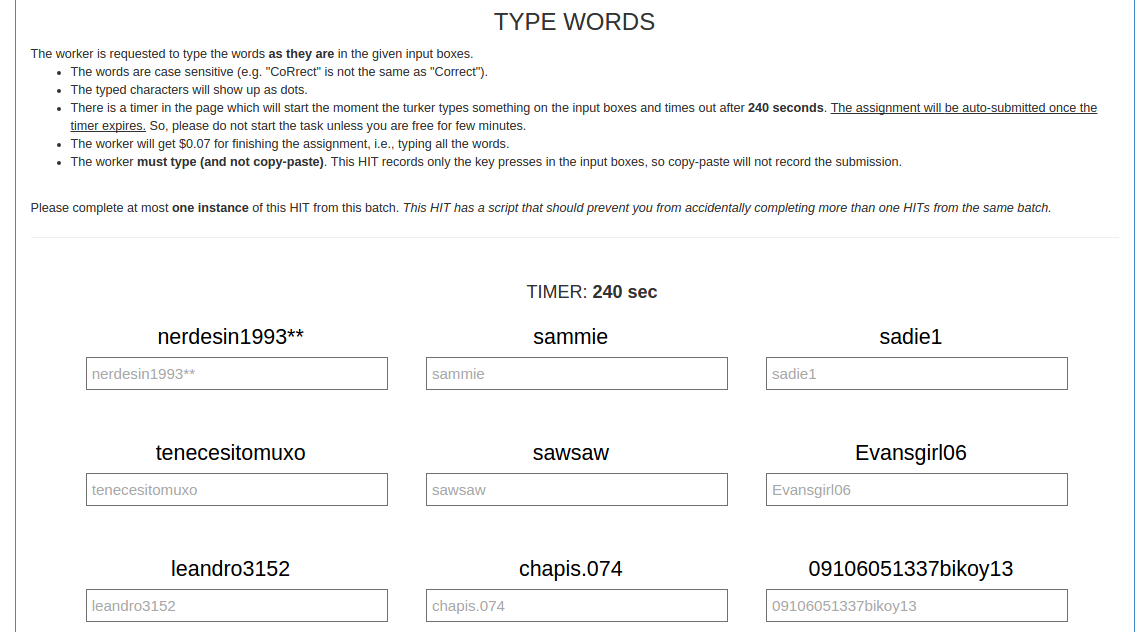
\includegraphics[width=\textwidth]{images/HIT}
%\includegraphics[width=0.45\textwidth]{images/HITcapslock1}
%\includegraphics[width=0.45\textwidth]{images/HITcapslock2}
\caption{An example MTurk HIT for password typo study ({\bf top}). In the {\bf bottom} two figures the two types of caps-lock indicators are shown.}
\label{fig:hit}
\end{figure*}

%%% Local Variables:
%%% mode: latex
%%% TeX-master: "main"
%%% End:

%%%%%%%%%%%%%%%%%%%%%%%%%%%%%%%%%%%%%%%%%%%%%%%%%%%%%%%%%%%%%%%%%%%%%%%%%%%%%%%%
\subsection{Secure Sketches}
\label{app:secsketch}
Secure sketches and fuzzy extractors, explored by Dodis et
al.~\cite{dodisetal:2004,1543961}, are designed to generate
consistent, cryptographically strong keys from noisy secrets, such as
biometric data. They may also be applied to passwords, as
typographical errors in passwords can be modeled as noise.
Dodis~et~al.~proposed two ways to construct secure sketches for the
edit-distance metric space; see Section 7
of~\cite{dodisetal:2004}. They show how to use a low-distortion
embedding for the edit-distance metric given by Ostrovsky and
Rabani~\cite{ostrovsky2007low}, and also describe a relaxed embedding
for the edit-distance metric using $c$-shingles. The security losses
for these constructions, as given in Proposition 7.2 and Theorem 7.5
of~\cite{dodisetal:2004}, are
$t(\log F)2^{O\left(\sqrt{\log(n\log F)\log\log(n\log F)}\right)}$ and
$\lceil{n\over c}\rceil\log(n-c+1)-(2c-1)t\lceil\log(F^c+1)\rceil$
respectively. Here, $n$ is the size of the password, $F$ is the
alphabet size, $t$ is the number of errors/edits tolerated, and $c$ is
a construction parameter denoting the size of the shingles. In our
setting, typical values would be $n=8$, $t=1$, and $F=96$. The value
of $c$, according to Theorem 7.4, should be 1 in our setting (and the
loss is an increasing function in $c$). Given these parameters, the
entropy loss of the two secure sketches would be $\approx 91$~bits and
$\approx 31$~bits respectively. The min-entropy of real world password
distributions is only about $\le 8$~bits~\cite{bonneau12}. Thus known
constructions provide no security guarantees in our context, and
providing proven constructions that do would seem to require new
techniques.




%% \begin{figure*}[t]
%%   \centering
%%   \small
%%   \begin{tabular}[t]{p{2.0in}lrrrr}
%%     \toprule
%%     \multirow{2}{*}{\textbf{Typo type}}     & \multirow{2}{*}{\textbf{Corrector}} & \multicolumn{3}{c}{\textbf{\% of typos}}\\\cline{3-6}
%%     &&{\bf general} & \pbox{1in}{\bf general\\(adjusted)} & \pbox{.8in}{\bf touchscreen \\device} & {\bf (New) \% of typos}\\\midrule
%%     Case of all letters flipped & \swcall & 30.9\% & 9.5\% & 8.3\% & 17.8\%\\
%% %    \midrule
%%     Case of first character flipped & \swcfirst &3.8\% & 4.6\% & 4.8\% & 7.8\% \\
%% %    \midrule
%%     Added extra character at the end & \rmlast &3.5\% & 4.6\% & 6.6\% & 3.7\%\\
%% %    \midrule
%%     Added extra character at the front & \rmfirst &  1.0\% & 1.3\% & 1.1\% & 1.1\%\\
%% %    \midrule
%%     Missed shift key for the last symbol &  \dtoslast & 0.2\% & 0.2\% & 0.0\% & 0.1\%\\
%%     % \midrule
%% %    \midrule
%%     Proximity errors & n/a & 17.3\% & 22.7\%  & 29.6\% & 19.0\%\\
%%     %Character replaced w/ nearby character on US keyboard 
%% %    \midrule
%%     Transcription errors & n/a & 2.3\% & 3.1\% & 3.4\% & 3.0\%\\
%% %    \midrule
%%     Other errors & n/a & 41.0\% & 54.0\% & 45.7\% & 46.5\%\\ 
%%     % Upper case to Title case and vice verse  &  \upncap & 0.2 & 0.3\%\\
%%     % \rownumber. & \stodlast & Last character symbol-to-number & 1\%\\
%%     % Change the shift state of the last non-letter character & \swslast& 0.3\%\\
%%     \bottomrule
%%   \end{tabular}
%% % \hspace{0.2in}
%% %   \begin{tabular}[t]{lr}
%% %     \toprule
%% %     \textbf{Correctors} & \textbf{\% of typos}\\\midrule
%% %     \swcall & 8.3\%\\
%% %     \swcfirst & 4.8\%\\
%% %     \rmlast & 6.6\%\\
%% %     \rmfirst & 1.1\%\\
%% %     \dtoslast & 0.0\%\\
%% %     Proximity errors & 29.6\%\\
%% %     Transcription errors & 3.4\%\\
%% %     Other errors  & 45.7\%\\\bottomrule
%% %   \end{tabular}
  
%%   \caption{The top kinds of typos observed in our collected data from
%%     the MTurk experiment over 100,000 passwords drawn from Rockyou,
%%     out of which 5,554 were mistyped.  The column labeled corrector
%%     identifies a correction function that can be used to catch the
%%     associated class of typos, when possible.  The right three columns
%%     are the percentage of all typos that were of the indicated type.
%%     The column under general (adjusted) is the one we obtained after
%%     discounting the caps lock errors that propagate over other
%%     passwords in same HIT.  This brings down the total number of mistyped
%%     password to 4,125. The right most column shows the percentage of
%%     typos broken down by their types that we saw in the data collected
%%     from touchscreen devices.  We see 2,075 typos among 23,098 typing
%%     events. }
%% \label{fig:top10-typo}
%% \label{fig:top-typo-mobile}
%% \end{figure*}





%%% Local Variables:
%%% mode: latex
%%% TeX-master: "main"
%%% End:



%%%%%%%%%%%%%%%%%%%%%%%%%%%%%%%%%%%%%%%%%%%%%%%%%%%%%%%%%%%%%%%%%%%%%%%%%%%%%%%%
\subsection{Sanitizing Caps-Lock Errors}
\label{app:caps-lock-err}

As mentioned in the paper body, preliminary analysis of the data revealed that a large
fraction of errors was caused by accidental pressing of the caps-lock
key. Measuring the rate of caps-lock errors is more challenging than
for other typos, for two reasons. First, caps-lock key presses are not
recordable via keystroke logging, and thus not directly detectable
remotely.  Second, if the user engages the caps-lock key while typing
one password, there's a chance that it will remain on (erroneously)
while the next one is entered. In MTurk, if an individual worker is to
be permitted to enter more than one password---even across multiple
HITs---propagation of caps-lock typos across passwords is therefore
methodologically unavoidable. This second issue accounts for the
(artificially) high rate of caps-lock typos observed in our
experiments. We found that 76 HITs contributed to 1120 caps-lock
errors.

To adjust for the effect of such propagation errors in determining the rate of
caps-lock typos, we do the following. We define a caps-lock error as an
incorrect password which, when the cases of all the letters are
inverted, becomes correct. In sequentially processing the passwords in a HIT, we
use a variable {\sf CL-ERR} $\in \{{\tt 0}, {\tt 1}\}$ to denote a heuristic
determination as to whether the caps lock is in an error state 
when the user entered a password in a HIT. (An error state could either be that 
caps lock is on and the user should have typed lower-case letters, or caps lock is
off and the user should have typed upper case letters.) We initially let {\sf CL-ERR} =
${\tt 0}$. When we detect a caps-lock error in a password, we record it and
set {\sf CL-ERR} = ${\tt 1}$. If it is already the case that {\sf CL-ERR} =
${\tt 1}$ when we reach a password in a HIT, we discard the password. That is,
in such cases, we do not count it in our computation of error rates for any
typo. Additionally, for every password in a HIT, we determine (heuristically)
whether the caps lock has been turned off during entry of the password. If the
password contains at least one letter and the password was submitted correctly, 
then we set {\sf CL-ERR} = ${\tt 0}$. 

In general, the intuition here is that we keep track heuristically of whether
the caps-lock key appears to be engaged erroneously. If the entry of a password
in a HIT has been affected by the state of the erroneously engaged caps-lock
key, we treat it as ``tainted,'' and thus discard it from our experiment. (We
assume heuristically that caps-lock errors are independent of other typos. The
global effect of discarding ``tainted'' passwords and not recording typos they
contain in addition to caps-lock errors is small in any case.)

% Measuring the rate of such errors is more challenging than for other
% typos, for two particular reasons. First, caps lock key presses are
% not remotely detectable. We use a heuristic rule to determine whether
% the caps lock key was on during the entry of a password: If the
% password could be corrected by inverting the case of alphabetic
% characters, we deem the caps lock to have been on. A second difficulty
% is that caps lock engagement is the only form of typographical error
% that propagates across passwords.  We therefore estimate the rate of
% caps-lock-induced typos as follows. We treat every ``eligible''
% password as an independent experiment

% On investigating it in detail, we
% discovered an anomaly in our experimental approach, which is causing
% such a high count for caps lock related errors. The caps lock error,
% if not corrected, will spread over all the passwords in the HIT, and
% will be counted towards as caps lock error, even though this is not a
% realistic scenario for website login.  There are \fixme{70} HITs which
% contributes to \fixme{1000} caps lock errors. To remove this error, we
% adjusted our count of typos in the following way.  Whenever there is a
% continuous run of caps lock errors, we only considered the first
% password as a caps lock error and all the rest are considered as
% correct typing.  In figref{fig:top10-typo} we present both the
% percentages before the adjustment (second from the right column) and
% after the adjustment (right most column).

%%% Local Variables:
%%% mode: latex
%%% TeX-master: "main"
%%% End:

\subsection{Complexity and Typo Likelihood} 
\label{app:complexity}

Our MTurk experiments revealed a significant initial finding regarding the frequency
of typos. Typo rates in our study increased under the following three distinct
metrics relating to password complexity.

\paragraph{\em Lexical diversity in passwords:}
One might suspect that more lexically diverse passwords---ones that
include symbols, letters with different cases, numbers or some
combination thereof---would be more prone to typos.  We define four character classes: upper case letters,
lower case letters, digits, and symbols.  Now, based on how many of
the four classes of characters are present within a password we can
partition passwords into four buckets. For example, passwords
containing characters from only one of the four classes are binned as
bucket 1, passwords containing exactly two different classes of
characters are bucket 2, etc.  In our first sample of 100,000
passwords, there were very few lexically diverse passwords. RockYou has $<0.2\%$
passwords with characters from all of the four character classes.
So we sample with replacement 5,000 passwords for each bucket from
the empirical distribution of passwords in RockYou restricted to the
passwords corresponding to the bucket. We performed the same
typing experiment as described before but with new HITs created from these
newly sampled passwords. In the left graph of~\figref{fig:complexity-typo}, we present the percentage of passwords in each bucket that were mistyped.


%That said, trends we discuss
%below hold as well when restricting attention to just unique passwords. 

%\rcnote{Some discussion for this result. This is quite counter intuitive}

% Obviously this is biased by the way we sampled, which is
% according to RockYou --- more frequently typed passwords were typed more often.
% If one normalizes the frequencies of typos for a particular password 
% by the number of times it was typed, a different story emerges. This is shown in
% the right of \figref{fig:popularity-typo}. We warn, however, that most of these
% results are not significant in that most passwords were only typed a single
% time. 

%We can see that the bulk of passwords
%for the passwords grouped by their frequency of occurance in the 
%RockYou dataset. \tnote{Insert analysis}
%%%%%%%%%%%%%%%%Typing speed, time, length and typo %%%%%%%%%%%%%%%%%%%%%%%%%%%%%%%%%%%%%%%%%%
\begin{figure*}[t]
\gamesfontsize
  \begin{center}
%    \hspace{0.3in}
    \begin{tikzpicture}[scale=0.4]
      \begin{customlegend}[
        legend columns=2,
        legend style={
          align=left,
          draw=none,
          column sep=2ex,
          font=\fontsize{8}{4}\selectfont
        },
        legend entries={Samples~~~, Typos}]
        \addlegendimage{ybar, ybar legend, blue!50}
        \addlegendimage{mark=*,red!90}   
      \end{customlegend}
    \end{tikzpicture}
  \end{center}
  \vspace{0.01in}
  \centering
  \plotmturk{\complexitytypotable}{cmplcl}{xlabel={\large
      Lexical diversity}, ylabel={\large \% of samples in each
      bucket}}{totalsample}{ylabel={},
    ymax=0.20}{typo}{}{}
%   \hspace{-0.3in}
  \plotmturk{\lengthtypotable}{length}{xlabel={\large Password length}, ylabel={}}{totalsample}{ylabel={}, ymax=0.2}{typo}{}{}
 \plotmturk{\populartypotable}{freqrange}{xlabel={\large Popularity (RockYou frequency)}, ylabel={}}{totalsample}{ylabel={\large Probability of typo}, ymin=0.01, ymax=0.10}{typo}{}{}


%  \plotmturk{\typingtimetypo}{typingtime}{Avg.~time required to type (sec)}{totalsample}{}{typoa}{}{}{}  
%   \hspace{-0.3in}
 \caption{Three experiments showing typo frequency relative to various partitions of passwords into buckets. Bucket size is indicated on the left of each figure, and corresponding typo rates on the right. {\bf(Left)}   Passwords are partitioned into four buckets based on
  diversity of character types. For each bucket we report
    the percentage of samples (blue bars) that fall in that bucket and
    what fraction of those samples are mistyped (red line).
{\bf (Middle)} Passwords are categorized into buckets by increasing order of length.  {\bf(Right)} 
    Passwords are assigned to buckets by decreasing
    frequency (increasing unpopularity) in RockYou. Bucket frequency ranges are selected so that each bucket has roughly an equal
    number of samples. %The frequency ranges that we considered include 
   % \{$\le 1$, $2-11$, $12-211$, $\ge212$\}.   
  }
  \label{fig:complexity-typo}
  \label{fig:length-typo}
  \label{fig:popularity-typo}
\end{figure*}


\paragraph{\em Password length:}
We divide passwords into five groups based on their lengths, namely
$\le5$, 6--7, 8--9, 10--11, and $\ge12$. For each class, we compute
the percentage of samples that lie in that class, along with the
percentage of passwords in those samples that were mistyped.  In the
middle graph of \figref{fig:length-typo} we show these numbers for
each of the length groups. As one might expect, typo likelihood grows with password length. 

\paragraph{\em Password popularity:} We sort the list of sampled
passwords for our MTurk experiment based on their frequency counts in
the RockYou leak. (Ties were broken alphabetically.) We then split the
passwords into four buckets, adjusting their corresponding frequency
ranges to ensure that buckets are of roughly equal size. (Some
unevenness was unavoidable, as many passwords occur only once in the
Rockyou leak.) For each bucket, we present the number of mistyped
passwords in the right graph of \figref{fig:popularity-typo}.  We can
see the clear trend that passwords that are popular among RockYou
users are more likely to be typed correctly.  For example, passwords
used by more than 211 users are 1.5 times more likely to mistyped than
those used by only one user.


\paragraph{Discussion: password typing complexity.}  As noted above,
lexical diversity, length, and popularity are related
metrics. Inspection of the passwords within the various buckets used
in the charts of \figref{fig:popularity-typo} reveals that there is
significant overlap between them. As one example, 18\% of the
passwords with lexical-diversity bucket 4 {\em both} have length
$\ge 12$ {\em and} are unpopular ($f = 1$).

The three metrics together highlight different
aspects of the underlying and intuitive trend: some passwords are more
difficult to type than others. It appears, moreover, that typos are more likely to
surface in harder-to-guess passwords. Consequently, typo correction
could help encourage users to adopt stronger passwords by easing the
use of such passwords. We leave rigorous study
of this hypothesis to future work, but note that it offers further
potential motivation for our work.



%%% Local Variables:
%%% mode: latex
%%% TeX-master: "main"
%%% End:

\subsection{Typist Speed and Typo Rate}
\label{sec:typistspeed}

As an enhancement of our experimental results in Section~\ref{sec:mturk}, we report on two experiments that provide further illumination of password features that lead to typos. These experiments further emphasize our observation  that typo rates appear to increase with password complexity.

\paragraph{\em Typist and typo likelihood.} 
In our MTurk experiments, we timestamped each character as
it was typed during the experiments.  We sorted the workers based on their
average typing speed (characters-per-minute) and binned workers into four
quartiles. For each quartile, we consider the subset of passwords that were
typed by the typists whose speed falls in that quartile, and we compute the
fraction of passwords that were mistyped in that subset. The data is reported in
\figref{fig:typespeed-typo}.  We found that slow typists make more mistakes than
faster typists. It could be that faster typists are also more skilled and so
less likely to make mistakes.

%%%%%%%%%%%%%Typing speed and typo%%%%%%%%%%%%%%%%%%%%%%%%%%%%%%%%%%%%%%%
\begin{figure}[t]
  \centering
  \plotmturk{\tspeedtable}{tspeed}{xlabel={\large
      Avg.~typing speed (cpm)}, ylabel={\large \%of samples in each
      class}}{totalsample}{ylabel={\large Probability of typo},
    ymax=0.1}{typo}{~~Samples}{~~Typos}
  \caption{ The workers are divided into four quartiles based on their
    typing speed, and for each quartile we report the percentage of
    passwords that were mistyped.}
  \label{fig:typespeed-typo}
\end{figure}



\paragraph{\em Password entry time.} We binned the passwords into four quartiles based on the time required
to type those passwords. The fraction of typos in each of that quartile
is reported in the middle chart of \figref{fig:typetime-typo}. 
Passwords that required more time on average to type are more likely to be
mistyped. 
%%%%%%%%%%%%%Password popularity and typo%%%%%%%%%%%%%%%%%%%%%%%%%%%%%%%%%%%%%%%
\begin{figure}[t]
  \centering 
  \plotmturk{\typingtimetypo}{typingtime}{xlabel={\large Avg.~time required to type (sec)}, ylabel={\large \% of typos in each  cohort}}{totalsample}{ylabel={\large Probability of typo}, ymax=0.1}{typo}{}{}

    \caption{ 
   % Probability of a password being mistyped is positively
   % correlated with the amount of time spent in typing the
   % password. 
    Passwords are divided into four quartiles based
    on the amount of time spent by workers to type them, and then compute
    the fraction of passwords mistyped in each quartile. }
  \label{fig:typetime-typo} 
\end{figure}

%%% Local Variables:
%%% mode: latex
%%% TeX-master: "IEEEtran.cls"
%%% End:

%%%%%%%%%%%%%%%%%%%%%%%%%%%%%%%%%%%%%%%%%%%%%%%%%%%%%%%%%%%%%%%%%%%%%%%%%%%%%%%%
\subsection{Computing $\greedylambda_q$}
\label{sec:faster-attack}

%%%%%%%%%%%%%%%%%%%%%%%%%%%%%%%%%%%%%%%%%%%%%%%%%%%%
We start by showing that computing the optimal $q$ guesses to make
against a relaxed checker is NP-hard in general. Later, we present an
efficient approximate algorithm for the problem.


\begin{definition} {\bf Best-$q$-guess.} Given a function
  $\ball:\strings \rightarrow \PW^*$, a password distribution
  $\pwprob$ over $\PW\subseteq\strings$, and a query budget $q$, find
  a $q$-size subset $P\subseteq \strings$, such that
  $\sum_{\pw\in C'}\pwprob(\pw)$ is maximized, where
  $C' = \bigcup_{\pwtypo\in P}\ball(\pwtypo)$.
\end{definition}

\begin{definition} {\bf Maximum coverage problem.} Given a ground set
  $E=\{e_1, e_2,\ldots e_n\}$, a collection of $m$ subsets of $E$,
  $S = \{S_1, S_2,\ldots,S_m\}$, and a weight function
  $\gamma:E\rightarrow \R^+$ that assigns weights to each element
  $e\in E$, find a subset $C\subseteq S$ of size $k$, such that
  the following quantity is maximized, $ \sum_{e\in C'}\gamma(e) $,
  where $C' = \bigcup_{S_i\in C} S_i$.
\end{definition}

The maximum coverage problem is known to be
NP-hard~\cite{feige1998threshold}. We can thus prove the
following theorem.

\begin{theorem}
  \label{th:finding-best-q}
  If there is a polynomial time algorithm for best-$q$-guess, there
  exists a polynomial time algorithm for maximum coverage
  problem.
\end{theorem}

\noindent\proof We shall show a polynomial time reduction from the maximum coverage
problem to the best-$q$-guess problem. To start with, we are given an
instance of maximum coverage problem with $(E, S, \gamma, k)$, and we
want to construct an instance of best-$q$-guess problem.  To do so, we
set $\PW = E$ and probability $\pwprob$ as proportional to
$\gamma$. (We might have to normalize $\gamma$ to make it a
probability distribution.)  The function
$\ball:\strings \rightarrow \PW^*$ is defined as follows.  First add
to $\strings$ a set $W^* = \{\pwtypo^*_i\}_{i=1}^m$, with
$\pwprob(\pwtypo^*_i) = 0$, and for each $S_i\in S$, set
$\ball(\pwtypo^*_i) = S_i \,\bigcup\, \{\pwtypo^*_i\}$. For all other
$\pwtypo\in \strings\setminus W^*$, let
$\ball(\pwtypo) = \{\pwtypo\}$. This is a valid instance of the
best-$q$-guess problem, and if we can find an polynomial time
computable solution to this, we can solve the maximum weighted set
cover problem in polynomial time. \qedsym

% The best
% guesses output by the solver can be mapped back to the best set of $k$
% sets which maximizes the cumulative weight.  The reduction is in
% polynomial time.


% where $\pwtypo_i\in \strings$.

%  For Best-$q$-guess problem
% we have a checker $\checker$ that checks every password in a ball
% $\ball(\pwtypo)\subseteq\PW$ on any submitted password $\pwtypo$. Let
% $E=\PW$ be the set of elements, and
% $S_i = \ball(\pwtypo_i)\subseteq \PW$. Now, in our context
% $S = \{\ball(s)\cap\PW\,|\,s\in \strinsg\}$. The weight function is
% $\pwprob$ that assigns a probability to each $\pw\in \PW$.  The
% problem is asked to find a set $P\subset\strings$ of size $q$ such
% that $\sum_{\pw\in\C'}\pwprob(\pw)$ is maximized, where
% $C'=\bigcup_{s\in P}\ball(s)$.


% Given any set cover problem with parameter $(E, S, \gamma, k)$ we can
% reduce that to optimal $q$-guessing problem by the way we just
% described. So, if there is a polynomial time algorithm for the later
% than so would be for the former. But, maximum weighted set cover is a
% well known NP-hard problem, so is $q$-guessing problem.


Nevertheless, a greedy algorithm can achieve
$(1-{1\over e})$ times the optimal $\fuzzlambda$ value and, as shown by  Feige~\cite{feige1998threshold,nemhauser1978analysis}, yields
an optimal approximation
for the maximum coverage problem. Na\"{i}ve implementation of this
greedy algorithm for best-$q$-guess, however, requires searching over
exponentially many strings in $\strings$. We can exploit the fact that in our setting, a small number of correctors are used, and these correctors are efficiently invertible. Additionally, password weights are highly non-uniform. Thus it is efficient to enumerate all balls above a certain threshold weight, yielding the efficient implementation of Feige's greedy
approximation algorithm specified in \figref{fig:attack-algo}. The algorithm intuition is this: as an invariant, in any iteration of the
external while loop, all new balls (balls of $\pwtypo$) pushed onto
the heap have max-weight password $\pw$, and
hence total weight $\le b\cdot \pwprob(\pw)$. This observation enables a global selection of balls in weighted order.


\iffalse
Here we give an algorithm for more efficiently computing $\greedylambda_q$. We
also discuss more the relationship between finding optimal query strategies and 
the weighted max set cover problem. 

Recall the greedy algorithm we sketched in 
\secref{subsec:security}. The problem with that algorithm is it iterates
over all the strings in the set $\strings$ which could be huge, and
%the ball around many of those strings will have zero induced
probability mass.  

In our game setting let $\checker$ the checking algorithm which uses
$\typoset$ correctors. The attacker assumes that the distribution of
passwords is $\pwprob$.  Note if $\pwprob$ is indeed the same as the
real password distribution then we call this attacker an exact-knowledge
attacker, otherwise an estimating attacker.  For a submitted password
$\pwtypo$, recall $\ball(\pwtypo)$ is the set of password that is
checked by the checker.  We define another variable called the
neighbor of a password $\pw$, which denotes the set of
$\pwtypo\in\strings$ which contain $\pw$ in their balls.  Let
$n = \max_\pw{|\nh{\pw}|}$, $b = \max_{\pwtypo} |\ball(\pwtypo)|$, and
$A = \{\pwtypo \in \strings \:|\: \exists \pw\in\PW,\,
\pwprob(\pw)>\varepsilon \mbox{ and } \pwtypo\in\nh{w}\}$.
{\claim Given a checker $\checker$ that checks maximum $b$ passwords
  for a submitted password, and a password will end up being be
  checked by submitting at most $n$ different strings, the top $q$
  guesses can be found within top $(q-1)nb+1$ strings of $A$ sorted
  based on ball
  weights}.  \\
\Proof Let, $A'$ be the set of $(q-1)nb+1$ heaviest balls of A. Each
guess can result in removing at most $b$ passwords from the set $P$,
each of which, in turn, can affect the weights of maximum $n$
different balls in $A'$. So, each guess can decrease the weights of at
most $nb$ balls. So, after making $q-1$ guesses, at least one string
$\pwtypo'$ will remain in $A'$ whose weight is not changed over the
course of the algorithm, and by definition of $A'$, there cannot be
any ball in $A\setminus A'$ that has higher weight than the ball
$\pwtypo'$. So, the algorithm will never require to choose any string
from $A\setminus A'$.

The attacker can utilize the aforementioned claim to expedite the
search for the best guesses drastically. The modified algorithm is
given in~\figref{fig:attack-algo}. In the algorithm the external while
loop, will be iterated at most $(q-1)bn$ times.  Another observation
in the algorithm, that in the process of generating the potential
guess list $A$, the attacker can emit a guess if the ratio of the
heaviest ball in $A$ and the recently inserted password probability is
more than $b$.  The idea is the any subsequent ball can have weight at
most the weight of the current ball times the size of the maximum
ball. So, if that product is less than the weight of heaviest ball in
A, the heaviest ball will be the attacker's next best guess.  Note,
the value of the $\varepsilon$ is clear from the algorithm.

In the
worst case (if the password distribution is close to uniform) then the
time complexity will end up being checking all the passwords in $\PW$
times $nb$.  But in practice, thanks to very skewed distribution of
user chosen passwords, the attack will terminate much faster than
that.

\fi

% \rcnote{Why? All new balls will have
%   lower weight than $b\times$probability of current $\pw$.}
% for w in B(wtilde_m)
%    for wtilde in N(w)
%
%for w in {wtilde in A | \exists w in B(w_m) and wtilde in N(w)}
%

\begin{figure}[t]
  \centering
  \def\aindent{\hspace*{10pt}}
  \fpage{0.4}{
    \small
    \underline{nextPw()}\\
    \textnormal{Returns the passwords in $\PW$ in
    decreasing order of their probability $\pwprob$.}\\[3pt]
    \underline{FindGuesses$(q)$}\\[2pt]
    /* $\ball(\pwtypo) =$ ball around $\pwtypo$, and  $b = \max_\strings |\ball(\pwtypo)|$ */ \\
    /* $\nh{\pw} = \{\pwtypo \,|\, \pw\in\ball(\pwtypo)\}$ */\\
    $P\leftarrow \PW$\\
    $A\leftarrow$ MaxHeap() \aindent /* val$(\pwtypo) = \pwprob(\ball(\pwtypo)\cap P)$ */\\
    $g\leftarrow \phi$; \\
    do $\{$ \\
    \aindent $\pw \leftarrow \mbox{nextPw}()$\\
    \aindent $\pwtypo_m \leftarrow A.\mbox{popmax}()$\\
    \aindent while $\;\pwprob(\ball(\pwtypo_m)\cap P)\ge b\cdot\pwprob(\pw)\; \{$\\
    \aindent \aindent $g\leftarrow g\cup \{\pwtypo_m\}$\\
    \aindent \aindent $P \leftarrow P\setminus \ball(\pwtypo_m)$\\
    \aindent \aindent foreach $\;\pwtypo \in \{\pwtypo\in A\,|\, \ball(\pwtypo)\cap\ball(\pwtypo_m)\cap P \ne \phi\}\;$\\
    \aindent \aindent \aindent $A.\mbox{updateweight}\left(\pwtypo\right)$\\
    \aindent \aindent $\pwtypo_m \leftarrow A.\mbox{popmax}()$\\
    \aindent $\}$\\
    \aindent $A.\mbox{heappush}(\pwtypo_m)$\\
    \aindent foreach $\;\pwtypo \in \left(\nh{\pw}\setminus A\right)\; $\\
    \aindent \aindent $A.\mbox{heappush}(\pwtypo)$\\
    % \aindent \aindent if $\;A.\mbox{length}() > (q-1)nb\;$ $\{$\\
    % \aindent \aindent\aindent $\pwtypo' \leftarrow A.\mbox{popmin()}$\\
    % \aindent \aindent $\}$\\
    % \aindent $\}$\\
    \} while ($|g|<q$)\\
    return $g$
  }
  \caption{Figure presents a greedy algorithm to compute the best $q$
    guesses and thereby compute $\greedylambda_q$, for an attacker who
    estimates the the password distribution with $\pwprob$. % If the
    % estimated distribution matches with real distribution, we call the
    % attacker as optimal attacker, otherwise estimating attacker.
  }
  \label{fig:attack-algo}
\end{figure}











%%% Local Variables:
%%% mode: latex
%%% TeX-master: "main"
%%% End:

%%%%%%%%%%%%%%%%%%%%%%%%%%%%%%%%%%%%%%%%%%%%%%%%%%%%%%%%%%%%%%%%%%%%%%%%%%%%%%%%
\subsection{Proofs}
\label{app:proofs}

We restate and then prove the free correction theorem from~\secref{sec:free-thm}. 

\setcounter{theorem}{0}
\begin{theorem}[\textbf{Free Corrections Theorem}] Fix some password
  distribution $\pwprob$ with support $\PW$, a typo distribution
  $\typoprob$, $0<q<|\PW|$ and an exact checker $\exchecker$.
%If there exists $\pw \in \PW$ with a neighbor $\pwtypo$ for which
%$\pwprob(\ball(\pwtypo)) < \pwprob(\pw_q)$,  
Then for \opchecker with any set of correctors $\typoset$, it 
holds that $\fuzzlambda_q = \lambda_q$. 
\label{thm:free_corr2}
\end{theorem}

\noindent\emph{Proof:}
Let $\hat{S}$ be the optimal set of $q$ strings which maximizes the
total acceptance rate for the given checker $\opchecker$.  (Note that
the order in which the queries are made does not change the success
probability.)  Let
$\ball(S) = \mathop{\cup}_{\pwtypo\in S} \ball(\pwtypo)$ for some set
$S$ of strings in $\strings$.  Recall that
$\lambda_q = \sum_{i=1}^{q} \pwprob(\pw_i)$ is the sum of the
probabilities of $q$ most probable passwords in $\PW$. On the other
hand, $\fuzzlambda_q = \pwprob\left(\ball(\hat{S})\right)$.  The above
holds because $\ball(\pwtypo)$ is the set of passwords checked by
\opchecker for a given string $\pwtypo$.


The checker $\opchecker$ ensures that the cumulative probability mass of
any ball is less than or equal to $\pwprob(\pw_q)$ whenever the size
of the ball is more than 1, but, if the size is one, the cumulative
probability can be more than $\pwprob(\pw_q)$.  So, we split $\hat{S}$
into two distinct groups $\hat{S}_1$ and
$\hat{S}_{>1}$, where $\hat{S}_1$ is the set of all strings in $S$
whose ball sizes are exactly one, and
$\hat{S}_{>1} = \hat{S}\setminus \hat{S}_1$.  We can claim following two
inequalities.
\begin{align}
  \label{eq:1}
  \pwprob\left(\ball(\hat{S}_1)\right) &\le \sum_{i=1}^{|\hat{S}_1|}\pwprob(\pw_i)\\
  \label{eq:2}
 \pwprob\left(\ball(\hat{S}_{>1})\right)&\le |\hat{S}_{<1}|\pwprob(\pw_q)  \le \sum_{i=|\hat{S}_1|+1}^{q}\pwprob(\pw_i)
\end{align}
Equation~\eqref{eq:1} is true because the
$|\ball(\hat{S}_1)|=|\hat{S}_1|$, and the right hand side is the
highest cumulative probability that any set of that size can achieve under
$\pwprob$.  Equation~\eqref{eq:2} is true because of the facts that $\pwprob(\ball(\pwtypo))\le\pwprob(\pw_q)$  for all $\pwtypo\in\hat{S}_{>1}$, and $\pwprob(\pw_i)\ge\pwprob(\pw_q)$ for all $i\ge q$. 
So, by a union bound over $\ball(\hat{S}_{>1})$,  we can achieve that inequality. 
We can add the two inequalities to obtain our  desired result.
\bnm \pwprob\left(\ball(\hat{S})\right) = \pwprob\left(\ball(\hat{S}_1)\right)  + \pwprob\left(\ball(\hat{S}_{>1})\right) \le  \sum_{i=1}^q\pwprob(\pw_i)
\enm

% \noindent\emph{Case 1:}
% If $\hat{S} = \PW_q$, then by construction of $\opchecker$ every ball
% around strings in $\PW_q$ will only contain the string itself.
% So, $\cup_{\pwtypo\in\hat{S}}\ball(\pwtypo) = \hat{S} = \PW_q$, and $\fuzzlambda_q = \lambda_q$.\\

% \noindent\emph{Case 2:}
% Now, consider the case when $\hat{S} \ne \PW_q$, then there must exist
% at least one $\pwtypo\in\hat{S}\setminus\PW_q$, because
% $|\PW_q| = |S| = q$. If the ball around $\pwtypo$ contains more than
% one password, then $\opchecker$ ensures that the weight of that ball
% is $\le \pwprob_q$. This argument is true for all
% $\pwtypo\in\hat{S}\setminus\PW_q$. 


% this string $\pwtypo$, the ball $\ball{\pwtypo}$
% might contain more than one passwords, in that case their cumulative
% sum will be less than $\pwprob_q$.


% Applying a union bound we have
% that
% $\fuzzlambda_q \le \sum_{\pwtypo\in \hat{S}}\pwprob(\ball(\pwtypo))$.
% Now, because \opchecker enforces that it only corrects as many
% passwords as have cumulative mass up to $p(\pw_q)$, we have that
% $\pwprob(\ball(\pwtypo)) \le \max\{\pwprob(\pwtypo), p_q\}$.  Hence,
% \bnm \sum_{\pwtypo\in \hat{S}}\pwprob(\ball(\pwtypo)) \le
% \max\{\sum_{\pwtypo\in \hat{S}}\pwprob(\pwtypo),\, qp_q\} \enm As per
% our assumption, if $\fuzzlambda_q>\lambda_q$, \bnm
% \max\{\sum_{\pwtypo\in \hat{S}}\pwprob(\pwtypo),\, qp_q\}>\lambda_q
% \enm Here we arrive at a contradiction because neither of the terms on
% the left hand side can be bigger than $\lambda_q$. First, by
% definition, $\lambda_q$ is the set of $q$ strings which has largest
% cumulative probability under the probability distribution $\pwprob$,
% and so $\lambda_q\ge \sum_{\pwtypo\in S}\pwprob(\pwtypo)$, for any
% size-$q$ subset of $\PW$.  Second,
% $\lambda_q = \sum_{i=1}^q \pwprob(\pw_i) \ge q\cdotsm\pwprob(\pw_q)$
% because $\pwprob(\pw_i) \ge \pwprob(\pw_q)$ for all $i\le q$.  This
% proves that $\fuzzlambda_q\le \lambda_q$.

To show strict equality, simply observe that an attacker against \opchecker 
can always choose the $q$ most probable passwords to guess
and achieve a success rate of $\lambda_q$. Thus $\fuzzlambda_q=\lambda_q$.
\qedsym\\

\setcounter{theorem}{1}
\begin{theorem} Fix $q > 0$, a distribution pair
  $(\pwprob,\typoprob)$, and a corrector set $\typoset$. Define
  \opchecker to work over $\typoset$ and let $\checker$ work for a set
  of correctors $\typoset' \subseteq \typoset$. If
  $\secloss_q(\checker) = 0$, then
  $\utility(\checker) \le \utility(\opchecker)$.
\end{theorem}
\def\Bt{\tilde{B}}
\noindent\emph{Proof:} 
First recollect utility of any checker $\checker$ is defined as
\begin{align*}\label{eq:th3eq1}
\utility(\checker) &= \Pr[\ACC(\checker)\Rightarrow \true]\\
  & = \sum_{\pwtypo\in\strings}\sum_{\pw\in\ball(\pwtypo)}\pwprob(\pw)\cdot\typoprob_{\pwtypo}(\pw),
\end{align*}
where $\ball(\pwtypo)$ is the ball of $\pwtypo$ under $\checker$.

Let assume for contradiction that there exists a checker $\checker$
which uses only the correctors in $\typoset$, achieves a
$\secloss_q(\checker)=0$ and still beats the $\opchecker$ in utility,
that is, $\utility(\checker)>\utility(\opchecker)$. Let denote a ball
of $\opchecker$ by $B(\cdot)$ and a ball of $\checker$ by
$\Bt(\cdot)$.  So, if $\utility(\checker)>\utility(\opchecker)$, then
there exists at least one $\pwtypo\in\strings$ such that
\begin{equation}
  \label{eq:th3eq1}
  \sum_{\pw\in \Bt(\pwtypo)}\pwprob(\pw)\cdot\typoprob_{\pw}(\pwtypo) >\sum_{\pw\in B(\pwtypo)}\pwprob(\pw)\cdot\typoprob_{\pw}(\pwtypo).
\end{equation}
% If
% $\pwprob(\pwtypo)>0$, then $\pwtypo$ must be in $B(\pwtypo)$ and
% $\Bt(\pwtypo)$ to meet the correctness criteria.
Now, by construction, the optimal checker $\opchecker$ selects the
$\ball(\pwtypo)$ that maximizes the utility under the constraint that
no ball of size 1 has higher cumulative mass than $\pwprob(\pw_q)$.
Here by utility we mean the sum
$\sum_{\pw\in\ball(\pw)}\pwprob(\pw)\cdot\typoprob_{\pw}(\pwtypo)$. (See
Eqn.~\ref{eq:constraints}.)  The checker $\checker$ can achieve higher
utility only if it violates one of the two constraints
in~\eqref{eq:constraints}.  The first constraint, required for
completeness, is inviolable.  The second constraint determines
security; if $\pwprob(\Bt(\pwtypo))>\pwprob(\pw_q)$ when
$|\Bt(\pwtypo)|>1$, then the security loss $\secloss_q(\checker)>0$
according to Lemma~\ref{th:secloss}. Thus there cannot exist any
$\pwtypo\in\strings$ fulfilling Eqn.~\ref{eq:th3eq1}. Thus
the assumption $\utility(\checker)>\utility(\opchecker)$ is false.
\qedsym


\setcounter{theorem}{3}
\begin{lemma}
\label{th:secloss}
For any password and typo distribution pair ($\pwprob$, $\typoprob$), checker $\checker$, and parameter
$0<q<|\PW|$, if there exists a string $\pwtypo\in\strings$,
s.t. $|\ball(\pwtypo)|>1$ and
$\pwprob(\ball(\pwtypo))>\pwprob(\pw_q)$, then 
$\secloss_q > 0$.
\end{lemma}

\noindent\emph{Proof:}  Security loss $\secloss_q>0$ implies that
$ \fuzzlambda_q > \lambda_q$. Let $\PW_q = \{\pw_1, \ldots, \pw_q\}$ and recall that
$\lambda_q = \pwprob(\PW_q)$.  Recall too that:
\bnm \fuzzlambda_q = \max_{S\subseteq\strings} \pwprob(\ball(S)), \,\,\mbox{ where }|S|=q.\enm
% We shall prove this theorem by constructing a set $S$ of size $q$ such
% that $\pwprob(\ball(S))>\pwprob(\PW_q)$.
First set $S\leftarrow
(\PW_q\setminus\ball(\pwtypo))\cup\{\pwtypo\}$.
Clearly $\fuzzlambda_q\ge \pwprob(\ball(S))$.  If we look at the union
of balls of the strings in the set $S$,
\[
  \ball(S) \supseteq \PW_q\cup\ball(\pwtypo)
\]
\[  
  \Rightarrow\pwprob(\ball(S)) \ge \pwprob(\PW_q) + \pwprob(\ball(\pwtypo)\setminus\PW_q) 
\]
Now, if $\ball(\pwtypo)\setminus\PW_q\ne\phi$, then clearly $\fuzzlambda_q\ge p(\ball(S))>\pwprob(\PW_q)$, and so $\secloss_q>0$. 

If $\ball(\pwtypo)\setminus\PW_q=\phi$, then $|S| < q$, as
$|\ball(\pwtypo)|>1$. Thus as long as there exists a password
$\pw'\in \PW\setminus S$ such that $\pwprob(\pw')>0$, we can add
$\pw'$ to $S$, resulting in $\pwprob(\ball(S)) > \pwprob(\PW_q)$. This
concludes the proof.  \qedsym




%%% Local Variables:
%%% mode: latex
%%% TeX-master: "main"
%%% End:


\subsection{Toy Example of Poor Ball Estimation} 
\label{sec:example}

Consider the following toy 
example of the attacker's estimated distribution $\hat{\pwprob}$ and the actual 
challenge distribution $\pwprob$:

\begin{figure}[h]
  \centering
  {\tt\small
  \begin{tabular}[t]{lc}
    \multicolumn{2}{c}{\textnormal{Attacker's estimate}}\\
    \hline
    $\pw$ & $\hat{\pwprob}(\pw)$\\\hline
    123456 & $\nicefrac{1}{3}$\\
    password & $\nicefrac{1}{4}$\\
    Password & $\nicefrac{1}{4}$\\
    qwerty & $\nicefrac{1}{6}$\\
    \hline
  \end{tabular}
}
  {\tt\small
  \begin{tabular}[t]{lc}
    \multicolumn{2}{c}{\textnormal{Actual distribution}}\\
    \hline
    $\pw$ & $\pwprob(\pw)$ \\\hline
    123456 & $\nicefrac{1}{2}$\\
    password & $\nicefrac{1}{5}$\\
    Password & $\nicefrac{1}{5}$\\
    asdffghj & $\nicefrac{1}{10}$\\
    \hline
  \end{tabular}
}
\end{figure}
\noindent The best guess of the attacker against $\exchecker$ is
{\tt 123456}, which yields success rate $1/2$. 
If the attacker wants to optimize her guess in the presence of a typo tolerant
checker, e.g., $\checkerall$ with correctors $\toptwo$, the
she select as her first guess is {\tt password} (in whose ball {\tt Password} lies), yielding success probability only $2/5$. 



%%% Local Variables:
%%% mode: latex
%%% TeX-master: "main"
%%% End:

%%%%%%%%%%%%%%%%%%%%%%%%%%%%%%%%%%%%%%%%%%%%%%%%%%%%%%%%%%%%%%%%%%%%%%%%%%%%%%%%%
\subsection{Further Related Work}
\label{sec:relwork}

The study of password checking systems
originates with Morris and Thompson's seminal paper on the security of the UNIX
login system~\cite{morris}. Specifically they showed that a majority of
user-selected passwords were easily cracked via offline brute-force attacks:
given access to the hashes of passwords, one can repeatedly guess passwords and
check for consistency with the hash. A long line of subsequent studies have
confirmed that users tend to choose weak passwords~\cite{bonneau12,of,papers}. 
%As one notable example relevant to our results later, Bonneau instrumented the
%Yahoo!~login infrastructure, collected 69 million keyed hashes, and investigated
%a number of guessing metrics on the empirical distribution of passwords.  He
%proposes a metric called $\alpha$-guesswork for measuring the difficulty of
%mounting offline brute-force attacks relative to passwords chosen according 
%to some distribution.

There has been a wide array of research into memorability
and its relationship to security. Password strength
meters help signal to users when their password is
weak~\cite{others,komanduri2014telepathwords}, whereas password strength
policies force users to pick passwords according to some recipe that hopefully
makes them harder to guess.  Ur et al.~\cite{ur2012does} studied the effect of
password strength meters on user-selected passwords, and their results suggest
that only stringent meters can help increase security. somethin  Shay et
al.~\cite{shay2014can} showed that strength policies vary considerably in terms
of security and usability. Password update policies require users to change
passwords, and not reuse old passwords, but studies suggest that this
decreases usability without noticeably increasing
security~\cite{zhang:2010:security}.  

Some have suggested using passphrases --- sequences of words from some
dictionary --- instead of passwords (c.f.,~\cite{porter1982password}).
Human-chosen English passphrases exhibit similarly poor security as
human-chosen passwords~\cite{bonneau2012linguistic}.  The infamous
CorrectHorseStapleBattery-type passwords (first popularized by the xkcd comic
strip~\cite{xkcd}) suggest a user pick words from a dictionary and take the
password to be the concatenation of them. 

System-generated passwords are an alternative to user-chosen passwords. Here a
randomized computer program selects a password, and the user must memorize it.
In some systems the user is offered multiple passwords to choose from.  Bonneau
and Schechter~\cite{bonneau2014towards} show that in theory it is possible to
train users to memorize system-generated passwords with 56 bits of
unpredictability.  System-generated versions of the CorrectHorseStapleBattery
system have also been suggested~\cite{shay2012correct}, i.e., the system
randomly selects the words on behalf of the user. It was observed in this work
that one can perform some kinds of typo checking on behalf of the user, should
one pick an appropriate dictionary.

In the context of system-generated passwords,  Shay et
al.~\cite{shay2012correct} performed a study on Mechanical Turk and explore login
failure rates for generated random passwords, pronouncable passwords~\cite{gasser1975random} and
CorrectHorseStapleBattery-type passphrases. They report that
7.9\% of password entries failed due to capitalization typos, and another
15.2\% are simple typos (edit distance one). They also report a correlation of
typo likelihood with password/phrase length.
They suggest some simple strategies for tolerating typos here:
ignoring white spacing and, for CorrectHorseStapleBattery passphrases, checking
for the nearest dictionary word. Such a mechanism

\tnote{Need to add into the above a reference to that one-author tech report on
horsestaple type passphrases, and typo tolerance}


\begin{itemize}
\item Typo tolerant order independent Hashing.~\cite{bard2007spelling}
\item Error-correcting and hiding all partial information ~\cite{1543961}.
\item Fuzzy Extractor~\cite{dodisetal:2004,juelswattenberg:1999}.
\item Usability of Passphrases and error tolerance in that~\cite{shay2012correct}.
\end{itemize}




%%% Local Variables:
%%% mode: latex
%%% TeX-master: "main"
%%% End:

%\appendix
%\input{domainhiding}
%\input{kamouflageattack}
%\input{eval}
%\input{vaultsanitization}


\end{document}








%%% Local Variables:
%%% mode: latex
%%% TeX-master: t
%%% End:
